% CHAPITRE 3 — version dediee
\chapter{Conception et Architecture de la Solution}
\graphicspath{{Isipfe/Figures/}{diagramms/}}

\section{Introduction}

Ce chapitre formalise la conception de la plateforme de recrutement en reliant chaque besoin metier a une decision technique verifiable. Le travail de conception a ete mene sur les deux sites de l'entreprise (Bouarada et Zaghouan), avec un meme objectif: obtenir un systeme unique, securise, et exploitable sans divergence de regles entre acteurs.

La structure du chapitre suit une progression logique: planification et conduite Agile, cadrage des exigences, modelisation UML des flux, architecture logicielle, securite, donnees, puis gouvernance et automatisations. Chaque section ne decrit pas seulement un choix de conception; elle precise aussi les garde-fous retenus pour traiter les cas limites observes pendant le developpement.

\section{Demarche de conception et planification}

La conception a commence par une phase de planification pour eviter les iterations non maitrisees. Le cadrage a fixe un ordre de travail clair: collecte terrain, modelisation, validation technique, puis consolidation. A chaque etape, un livrable etait valide (diagrammes, decisions d'architecture, regles de gestion) avant le passage a la suivante.

\begin{figure}[H]
\centering
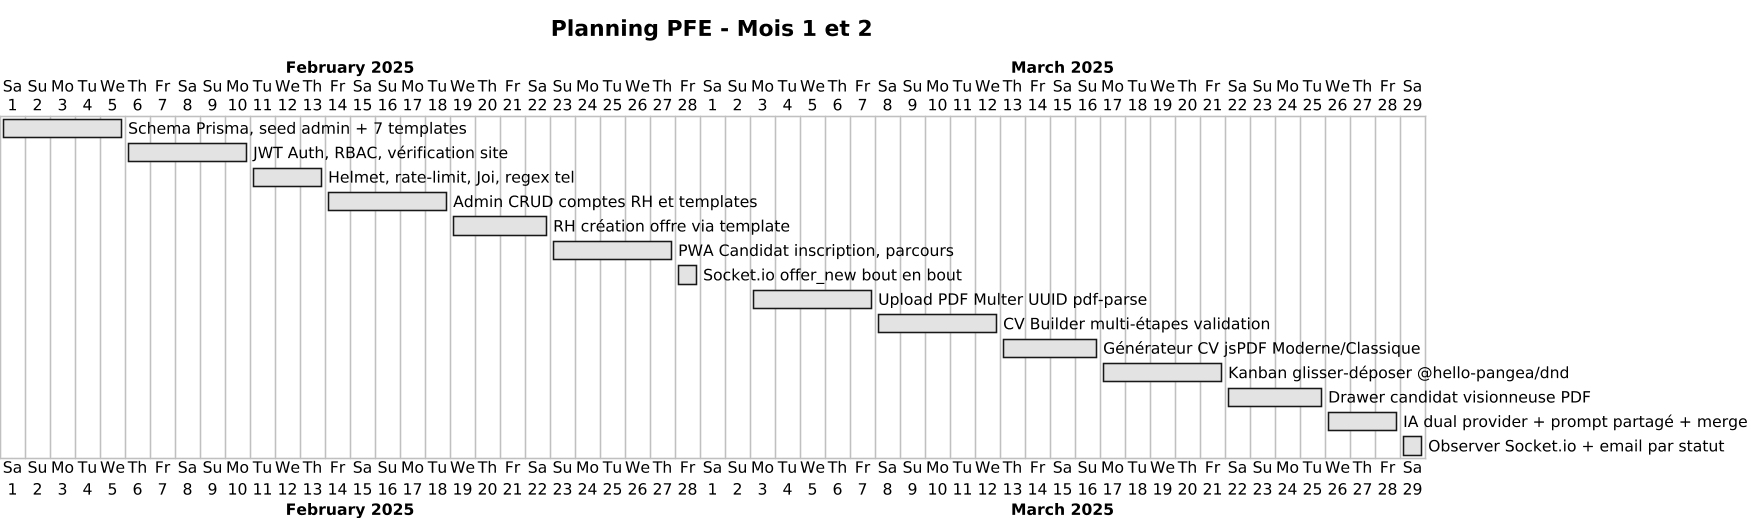
\includegraphics[width=0.86\textwidth]{gantt_mois_1_2.png}
\caption{Planification de conception -- Mois 1 et 2}
\end{figure}

Le premier Gantt couvre le cadrage : collecte des besoins, premiers modeles UML et validation des scenarios metier critiques.

\begin{figure}[H]
\centering
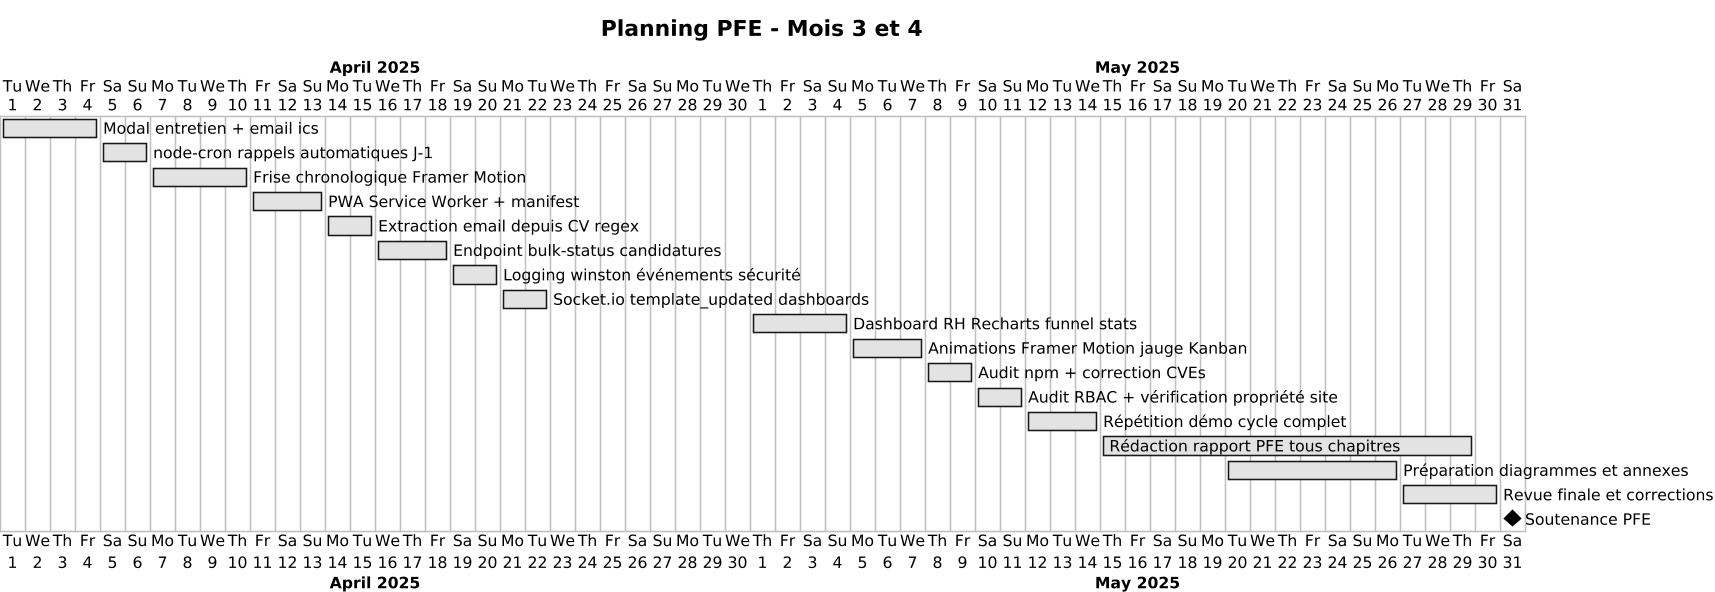
\includegraphics[width=0.86\textwidth]{gantt_mois_3_4.png}
\caption{Planification de conception -- Mois 3 et 4}
\end{figure}

Le second Gantt couvre la consolidation : finalisation de l'architecture, verrouillage du schema de donnees et preparation de la realisation.

\section{Conduite Agile du projet}

\subsection{Cadre Agile adopte}

Le cadre Scrum a ete adapte a l'echelle du projet PFE. Le product backlog a ete maintenu avec l'equipe RH, la planification s'est faite en cycles courts, et chaque sprint s'est termine par une revue fonctionnelle suivie d'une retrospective. Ce rythme a permis de corriger rapidement les ecarts entre maquette, logique metier et comportement reel de l'application.

\begin{table}[H]
\centering
\caption{Organisation Agile du chapitre de conception}
\begin{tabularx}{\textwidth}{|l|X|X|}
\hline
\textbf{Release} & \textbf{But} & \textbf{Sprints couverts} \\
\hline
Release 1 & Construire le flux recrutement de bout en bout (authentification, candidature, traitement RH) & S1, S2, S3, S4 \\
\hline
Release 2 & Stabiliser la gouvernance, la securite operationnelle et l'exploitation & S5, S6 \\
\hline
\end{tabularx}
\end{table}

\subsection{Sprint 1 -- Initiation et authentification}

\textbf{Vue technique} : ce sprint s'appuie sur les diagrammes d'inscription, verification email, connexion, generation des jetons et rotation des refresh tokens.

\begin{table}[H]
\centering
\caption{Backlog du sprint 1}
\begin{tabularx}{\textwidth}{|l|X|l|X|}
\hline
\textbf{ID} & \textbf{User story} & \textbf{Priorite} & \textbf{Critere d'acceptation} \\
\hline
S1-US1 & En tant que candidat, je cree un compte avec email valide. & Haute & Compte cree, verification requise avant connexion. \\
\hline
S1-US2 & En tant que candidat, je recois et renvoie un code de verification. & Haute & Verification email reussie, gestion expiration/rate-limit. \\
\hline
S1-US3 & En tant qu'utilisateur authentifie, je dispose d'un acces securise via JWT + refresh token. & Haute & Login, refresh, rotation et revocation fonctionnels. \\
\hline
\end{tabularx}
\end{table}

\begin{table}[H]
\centering
\caption{Tableau de taches du sprint 1}
\begin{tabularx}{\textwidth}{|l|X|l|X|}
\hline
\textbf{Tache} & \textbf{Description} & \textbf{Charge} & \textbf{Sortie} \\
\hline
S1-T1 & Endpoints \texttt{/auth/login}, \texttt{/auth/verify-email}, \texttt{/auth/resend}. & 2 j.h & API d'authentification candidate. \\
\hline
S1-T2 & Middleware de controle role/session + gestion cookies securises. & 1.5 j.h & Controle d'acces unifie RH/Admin/Candidat. \\
\hline
S1-T3 & Rotation refresh token + invalidation immediate compte inactif. & 1.5 j.h & Chaine de session robuste. \\
\hline
\end{tabularx}
\end{table}

\subsection{Sprint 2 -- Parcours candidat et depot de candidature}

\textbf{Vue technique} : ce sprint est aligne sur les diagrammes de creation CV (upload/builder), selection de CV et depot de candidature.

\begin{table}[H]
\centering
\caption{Backlog du sprint 2}
\begin{tabularx}{\textwidth}{|l|X|l|X|}
\hline
\textbf{ID} & \textbf{User story} & \textbf{Priorite} & \textbf{Critere d'acceptation} \\
\hline
S2-US1 & En tant que candidat, je gere ma bibliotheque de CV. & Haute & Upload PDF + builder + selection CV actifs. \\
\hline
S2-US2 & En tant que candidat, je postule a une offre avec un CV choisi. & Haute & Depot en base + accuse de prise en compte. \\
\hline
S2-US3 & En tant que systeme, je bloque les doublons candidat/offre. & Haute & Refus metier si candidature deja existante. \\
\hline
\end{tabularx}
\end{table}

\begin{table}[H]
\centering
\caption{Tableau de taches du sprint 2}
\begin{tabularx}{\textwidth}{|l|X|l|X|}
\hline
\textbf{Tache} & \textbf{Description} & \textbf{Charge} & \textbf{Sortie} \\
\hline
S2-T1 & Module CV: upload, extraction texte et mode builder. & 2.5 j.h & Donnees CV reutilisables dans le dossier candidat. \\
\hline
S2-T2 & Endpoint de soumission candidature avec validations metier. & 2 j.h & Depot candidature fiable et trace. \\
\hline
S2-T3 & Regle d'unicite candidature par offre. & 1 j.h & Prevention des dossiers redondants. \\
\hline
\end{tabularx}
\end{table}

\subsection{Sprint 3 -- Traitement RH, statuts et entretiens}

\textbf{Vue technique} : ce sprint mobilise les diagrammes de transitions Kanban, planification et outcome d'entretien.

\begin{table}[H]
\centering
\caption{Backlog du sprint 3}
\begin{tabularx}{\textwidth}{|l|X|l|X|}
\hline
\textbf{ID} & \textbf{User story} & \textbf{Priorite} & \textbf{Critere d'acceptation} \\
\hline
S3-US1 & En tant que RH, je deplace une candidature entre statuts valides. & Haute & Transitions controlees sans etat incoherent. \\
\hline
S3-US2 & En tant que RH, je planifie un entretien et je peux le replanifier. & Haute & Dates/horaires persistants et historises. \\
\hline
S3-US3 & En tant que RH, je saisis un resultat d'entretien. & Haute & Outcome (\texttt{pass}/\texttt{fail}/\texttt{no\_show}) enregistre et exploite. \\
\hline
\end{tabularx}
\end{table}

\begin{table}[H]
\centering
\caption{Tableau de taches du sprint 3}
\begin{tabularx}{\textwidth}{|l|X|l|X|}
\hline
\textbf{Tache} & \textbf{Description} & \textbf{Charge} & \textbf{Sortie} \\
\hline
S3-T1 & API de mise a jour statut avec normalisation des valeurs UI. & 1.5 j.h & Cycle d'etat coherent (\texttt{new} vers \texttt{reviewing}, etc.). \\
\hline
S3-T2 & Module planification entretien + edition/replanification. & 2 j.h & Workflow entretien complet. \\
\hline
S3-T3 & Enregistrement outcome et propagation metier. & 1.5 j.h & Decision RH tracee jusqu'aux etats finaux. \\
\hline
\end{tabularx}
\end{table}

\subsection{Sprint 4 -- Analyse IA dual-provider et temps reel}

\textbf{Vue technique} : ce sprint suit les diagrammes Puter.js, Gemini, fusion IA, normalisation backend et emission Socket.io.

\begin{table}[H]
\centering
\caption{Backlog du sprint 4}
\begin{tabularx}{\textwidth}{|l|X|l|X|}
\hline
\textbf{ID} & \textbf{User story} & \textbf{Priorite} & \textbf{Critere d'acceptation} \\
\hline
S4-US1 & En tant que RH, je lance une analyse IA sans bloquer le flux candidat. & Haute & Analyse asynchrone fonctionnelle. \\
\hline
S4-US2 & En tant que RH, je consulte un resultat fusionne et lisible. & Haute & Score + recommandation + justification coherents. \\
\hline
S4-US3 & En tant qu'utilisateur, je vois les mises a jour en temps reel. & Haute & Evenements Socket propages aux bons clients. \\
\hline
\end{tabularx}
\end{table}

\begin{table}[H]
\centering
\caption{Tableau de taches du sprint 4}
\begin{tabularx}{\textwidth}{|l|X|l|X|}
\hline
\textbf{Tache} & \textbf{Description} & \textbf{Charge} & \textbf{Sortie} \\
\hline
S4-T1 & Pipeline asynchrone IA cote backend + snapshot candidature. & 2 j.h & Analyse declenchee sans ralentir le depot. \\
\hline
S4-T2 & Fusion des resultats Puter.js/Gemini et persistance finale. & 2 j.h & Resultat IA unifie et exploitable RH. \\
\hline
S4-T3 & Evenements Socket (\texttt{status:changed}, \texttt{ai:analysis\_complete}). & 1.5 j.h & Synchronisation RH/candidat en temps reel. \\
\hline
\end{tabularx}
\end{table}

\subsection{Sprint 5 -- Gouvernance administrative}

\textbf{Vue technique} : ce sprint couvre la creation des comptes RH, leur cycle de vie, la gestion des templates et le broadcast admin.

\begin{table}[H]
\centering
\caption{Backlog du sprint 5}
\begin{tabularx}{\textwidth}{|l|X|l|X|}
\hline
\textbf{ID} & \textbf{User story} & \textbf{Priorite} & \textbf{Critere d'acceptation} \\
\hline
S5-US1 & En tant qu'admin, je cree et maintiens les comptes RH. & Haute & Creation, activation, desactivation et suppression maitrisees. \\
\hline
S5-US2 & En tant qu'admin, je gere les templates d'offres. & Moyenne & Templates reutilisables et edition centralisee. \\
\hline
S5-US3 & En tant qu'admin, je diffuse une information globale aux RH. & Moyenne & Message broadcast visible sur tableaux RH. \\
\hline
\end{tabularx}
\end{table}

\begin{table}[H]
\centering
\caption{Tableau de taches du sprint 5}
\begin{tabularx}{\textwidth}{|l|X|l|X|}
\hline
\textbf{Tache} & \textbf{Description} & \textbf{Charge} & \textbf{Sortie} \\
\hline
S5-T1 & Controleur admin pour comptes RH (CRUD logique + suppression definitive). & 2 j.h & Gouvernance comptes stabilisee. \\
\hline
S5-T2 & Gestion centralisee templates et publication guidee. & 1.5 j.h & Homogeneite de redaction des offres. \\
\hline
S5-T3 & Mecanisme broadcast admin vers rooms RH. & 1 j.h & Communication transversale fiabilisee. \\
\hline
\end{tabularx}
\end{table}

\subsection{Sprint 6 -- Stabilisation securite et exploitation}

\textbf{Vue technique} : ce sprint mobilise les diagrammes de rappels automatiques, notifications et architecture de securite en production.

\begin{table}[H]
\centering
\caption{Backlog du sprint 6}
\begin{tabularx}{\textwidth}{|l|X|l|X|}
\hline
\textbf{ID} & \textbf{User story} & \textbf{Priorite} & \textbf{Critere d'acceptation} \\
\hline
S6-US1 & En tant que RH, je recois des rappels automatiques fiables. & Moyenne & Rappels entretien emis a temps. \\
\hline
S6-US2 & En tant qu'equipe projet, nous fiabilisons les erreurs de flux. & Haute & Rollback UI/API propre et messages explicites. \\
\hline
S6-US3 & En tant qu'administrateur, je maitrise les acces sensibles. & Haute & Controles role/site et revocation effectifs. \\
\hline
\end{tabularx}
\end{table}

\begin{table}[H]
\centering
\caption{Tableau de taches du sprint 6}
\begin{tabularx}{\textwidth}{|l|X|l|X|}
\hline
\textbf{Tache} & \textbf{Description} & \textbf{Charge} & \textbf{Sortie} \\
\hline
S6-T1 & Cron de rappel entretien + marquage \texttt{reminderSent}. & 1 j.h & Rappels idempotents et tracables. \\
\hline
S6-T2 & Durcissement des routes sensibles (site ownership, role checks). & 1.5 j.h & Surface d'erreur securite reduite. \\
\hline
S6-T3 & Nettoyage des transitions et retours d'erreur front/backend. & 1.5 j.h & Comportements plus previsibles en exploitation. \\
\hline
\end{tabularx}
\end{table}

\subsection{Retrospective de release}

La retrospective montre que le decoupage en sprints a reduit les retours arriere tardifs. Les sprints 1 a 4 ont produit le flux metier principal (authentification, candidature, traitement RH, analyse), tandis que les sprints 5 et 6 ont porte la stabilisation operationnelle (gouvernance, securite, comportement en erreur). Cette repartition explique pourquoi la charge de fin de cycle reste moderee malgre l'ajout de contraintes de robustesse.

\begin{table}[H]
\centering
\caption{Synthese retrospective des sprints}
\begin{tabularx}{\textwidth}{|l|l|l|X|}
\hline
\textbf{Sprint} & \textbf{Charge prevue} & \textbf{Charge realisee} & \textbf{Observation} \\
\hline
S1 & 5 j.h & 5.5 j.h & Surcout leger du au durcissement de la securite session/token. \\
\hline
S2 & 5.5 j.h & 5 j.h & Bonne cadence grace au perimetre bien decoupe cote candidat. \\
\hline
S3 & 5 j.h & 5.5 j.h & Ajustements supplementaires sur transitions et outcomes entretien. \\
\hline
S4 & 5.5 j.h & 6 j.h & Complexite de fusion IA plus elevee que prevu. \\
\hline
S5 & 4.5 j.h & 4.5 j.h & Gouvernance admin stable, peu de reprises. \\
\hline
S6 & 4 j.h & 4.5 j.h & Stabilisation et tests de fiabilite plus longs en fin de cycle. \\
\hline
\end{tabularx}
\end{table}

\section{Cadrage des exigences}

\subsection{Structure des besoins}

Les besoins ont ete organises en quatre blocs: candidat, RH, administration et exigences transversales. Cette decomposition evite de confondre besoin metier et choix d'implementation.

\begin{figure}[H]
\centering
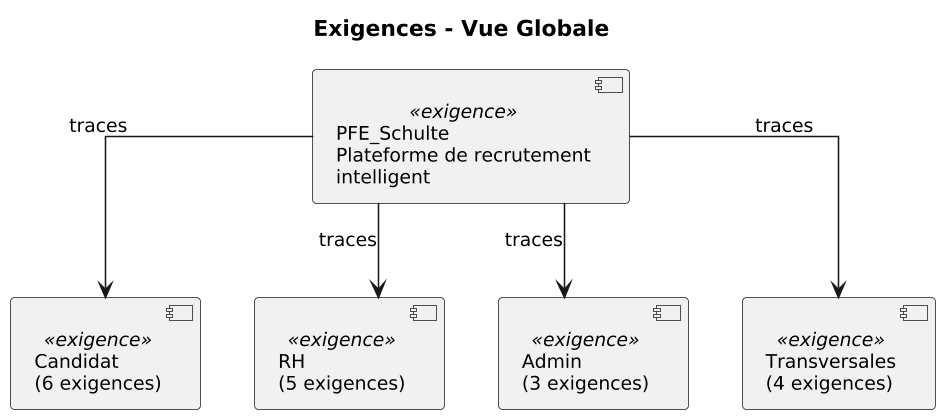
\includegraphics[width=\textwidth]{vue_globale_exigence_racine_categories.png}
\caption{Vue globale des exigences fonctionnelles et transversales}
\end{figure}

Le schema racine fixe le perimetre du produit. Nous y separons clairement ce qui est inclus et ce qui reste hors scope.

\begin{figure}[H]
\centering
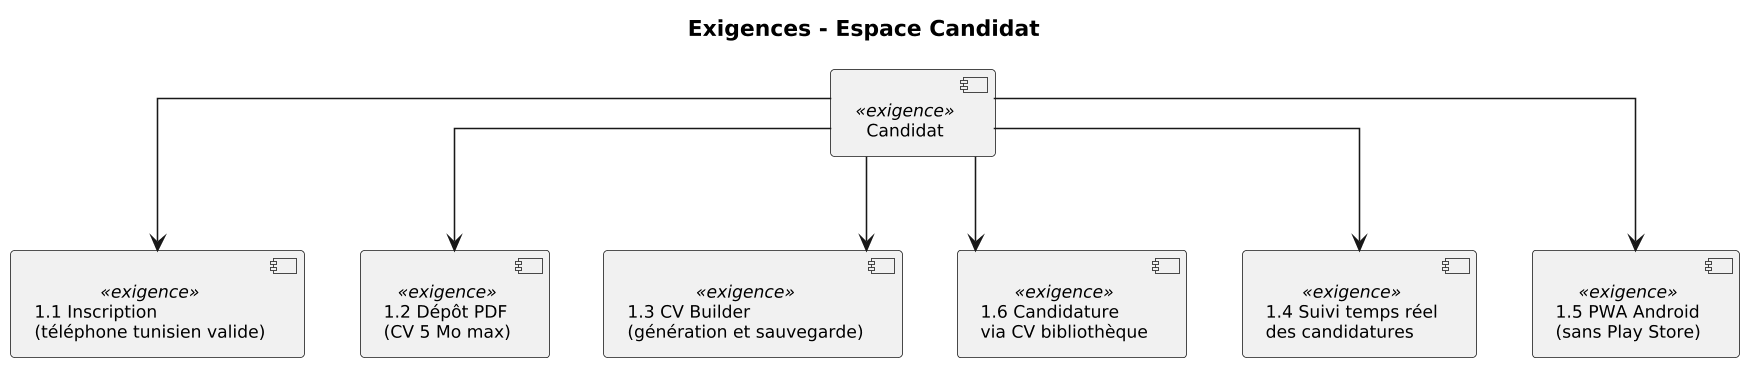
\includegraphics[width=\textwidth]{exigences_candidat_req.png}
\caption{Detail des exigences du module Candidat}
\end{figure}

Le diagramme candidat couvre toute la chaine : creation de compte, verification email, gestion des CV, depot puis suivi.

\begin{figure}[H]
\centering
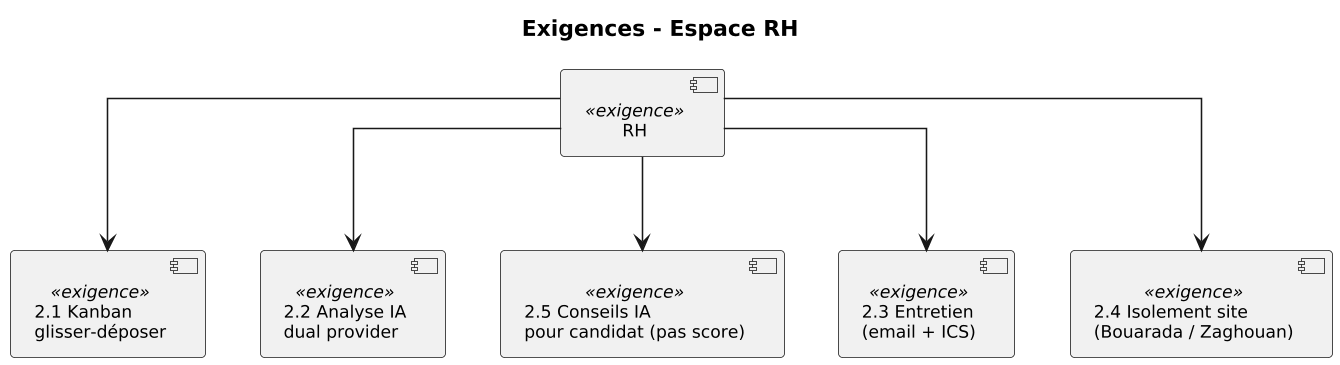
\includegraphics[width=\textwidth]{exigences_rh_req.png}
\caption{Detail des exigences du module RH}
\end{figure}

Le diagramme RH formalise le cycle metier : tri, changement de statut, planification d'entretien, puis decision finale.

\begin{figure}[H]
\centering
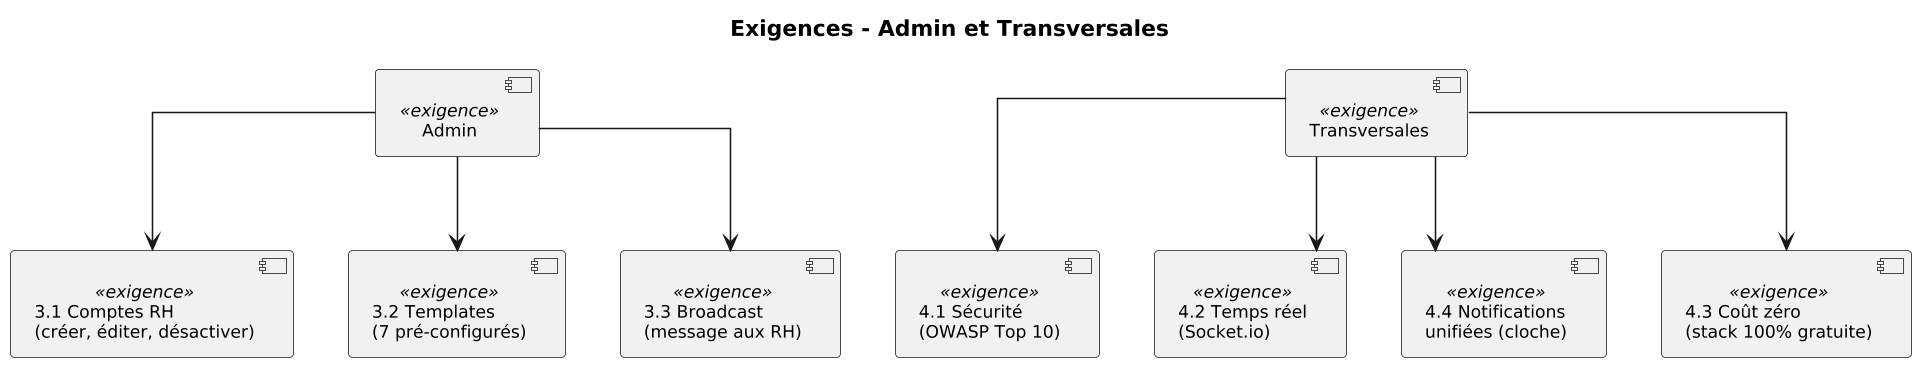
\includegraphics[width=\textwidth]{exigences_admin_transversales.png}
\caption{Detail des exigences Administration et contraintes transversales}
\end{figure}

Le diagramme admin regroupe la gouvernance (comptes RH, templates, diffusion) et les contraintes globales de securite et de tracabilite.

\subsection{Acteurs et priorites}

Le systeme repose sur trois acteurs: candidat, RH et administrateur. La separation des roles est stricte, avec isolation multi-site des actions RH. La priorisation suit le chemin critique metier: authentification, candidature, suivi RH, puis automatisations.

\section{Conception architecturale}

\subsection{Vue globale et decomposition technique}

L'architecture retenue est en couches (presentation, metier, persistance). Ce choix permet de faire evoluer les frontends sans destabiliser les regles metier.

\begin{figure}[H]
\centering
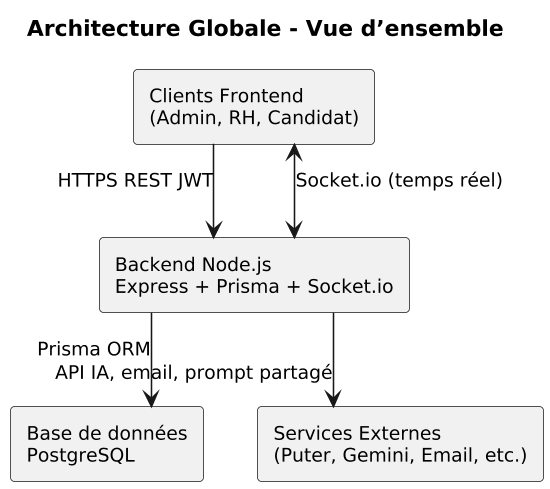
\includegraphics[width=\textwidth]{architecture_globale.png}
\caption{Architecture globale de la solution}
\end{figure}

La vue globale montre les trois applications et le backend central. Les flux principaux passent en HTTPS REST/JWT, puis en Socket.io pour les mises a jour temps reel.

\begin{figure}[H]
\centering
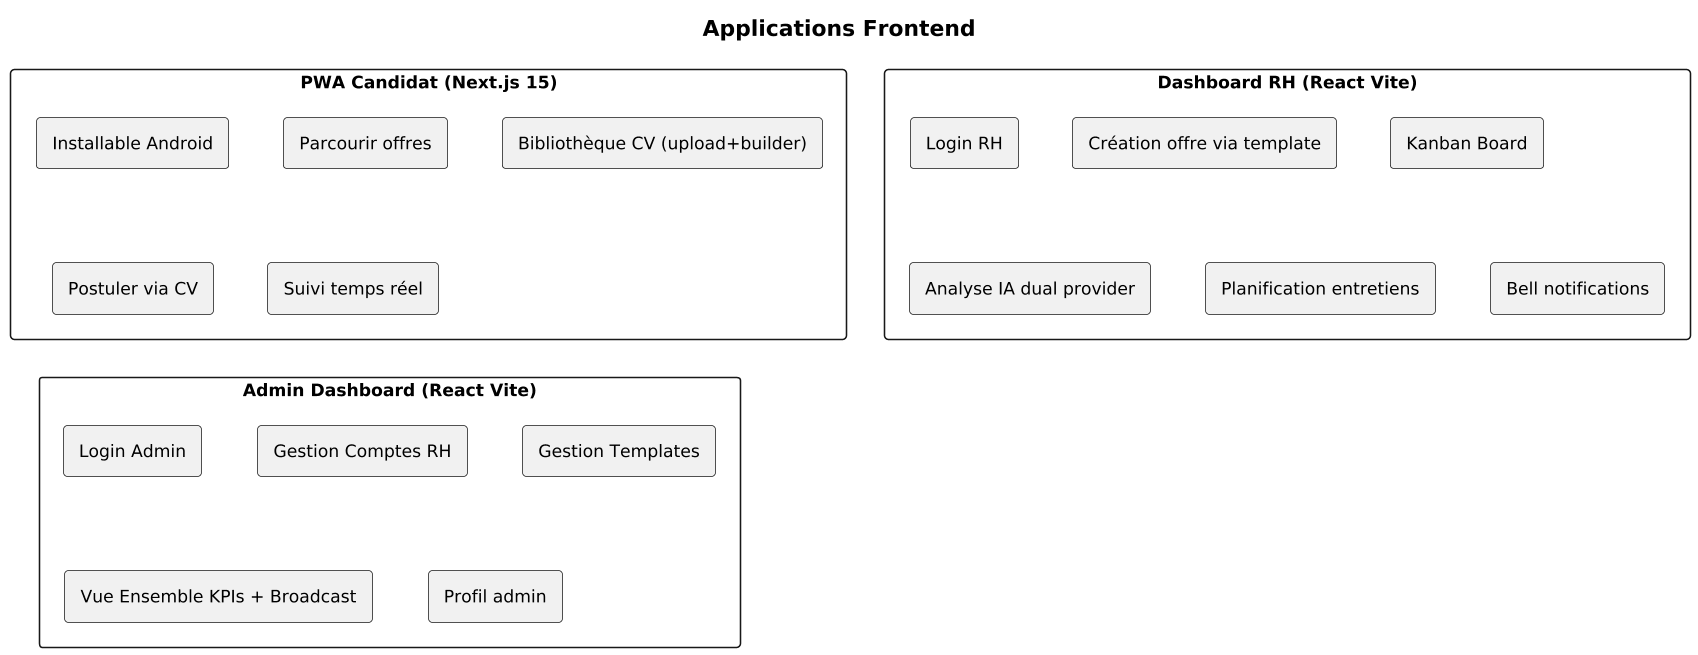
\includegraphics[width=\textwidth]{architecture_frontends.png}
\caption{Architecture des frontends (PWA candidat et interface RH/Admin)}
\end{figure}

La separation des interfaces par usage (PWA candidat, dashboard RH, dashboard admin) reduit la complexite fonctionnelle de chaque ecran.

Sur le plan client, les deux frontends n'appliquent pas la meme strategie de session. La PWA candidat utilise un intercepteur Axios avec file d'attente de rafraichissement (\texttt{refreshPromise}) afin qu'en cas de plusieurs erreurs \texttt{401} simultanees, une seule requete \texttt{/auth/refresh} soit envoyee avant rejeu des requetes en attente. L'interface RH privilegie une session par onglet via \texttt{sessionStorage} (avec fallback), ce qui limite les collisions d'etat quand plusieurs comptes sont ouverts sur le meme navigateur.

\begin{figure}[H]
\centering
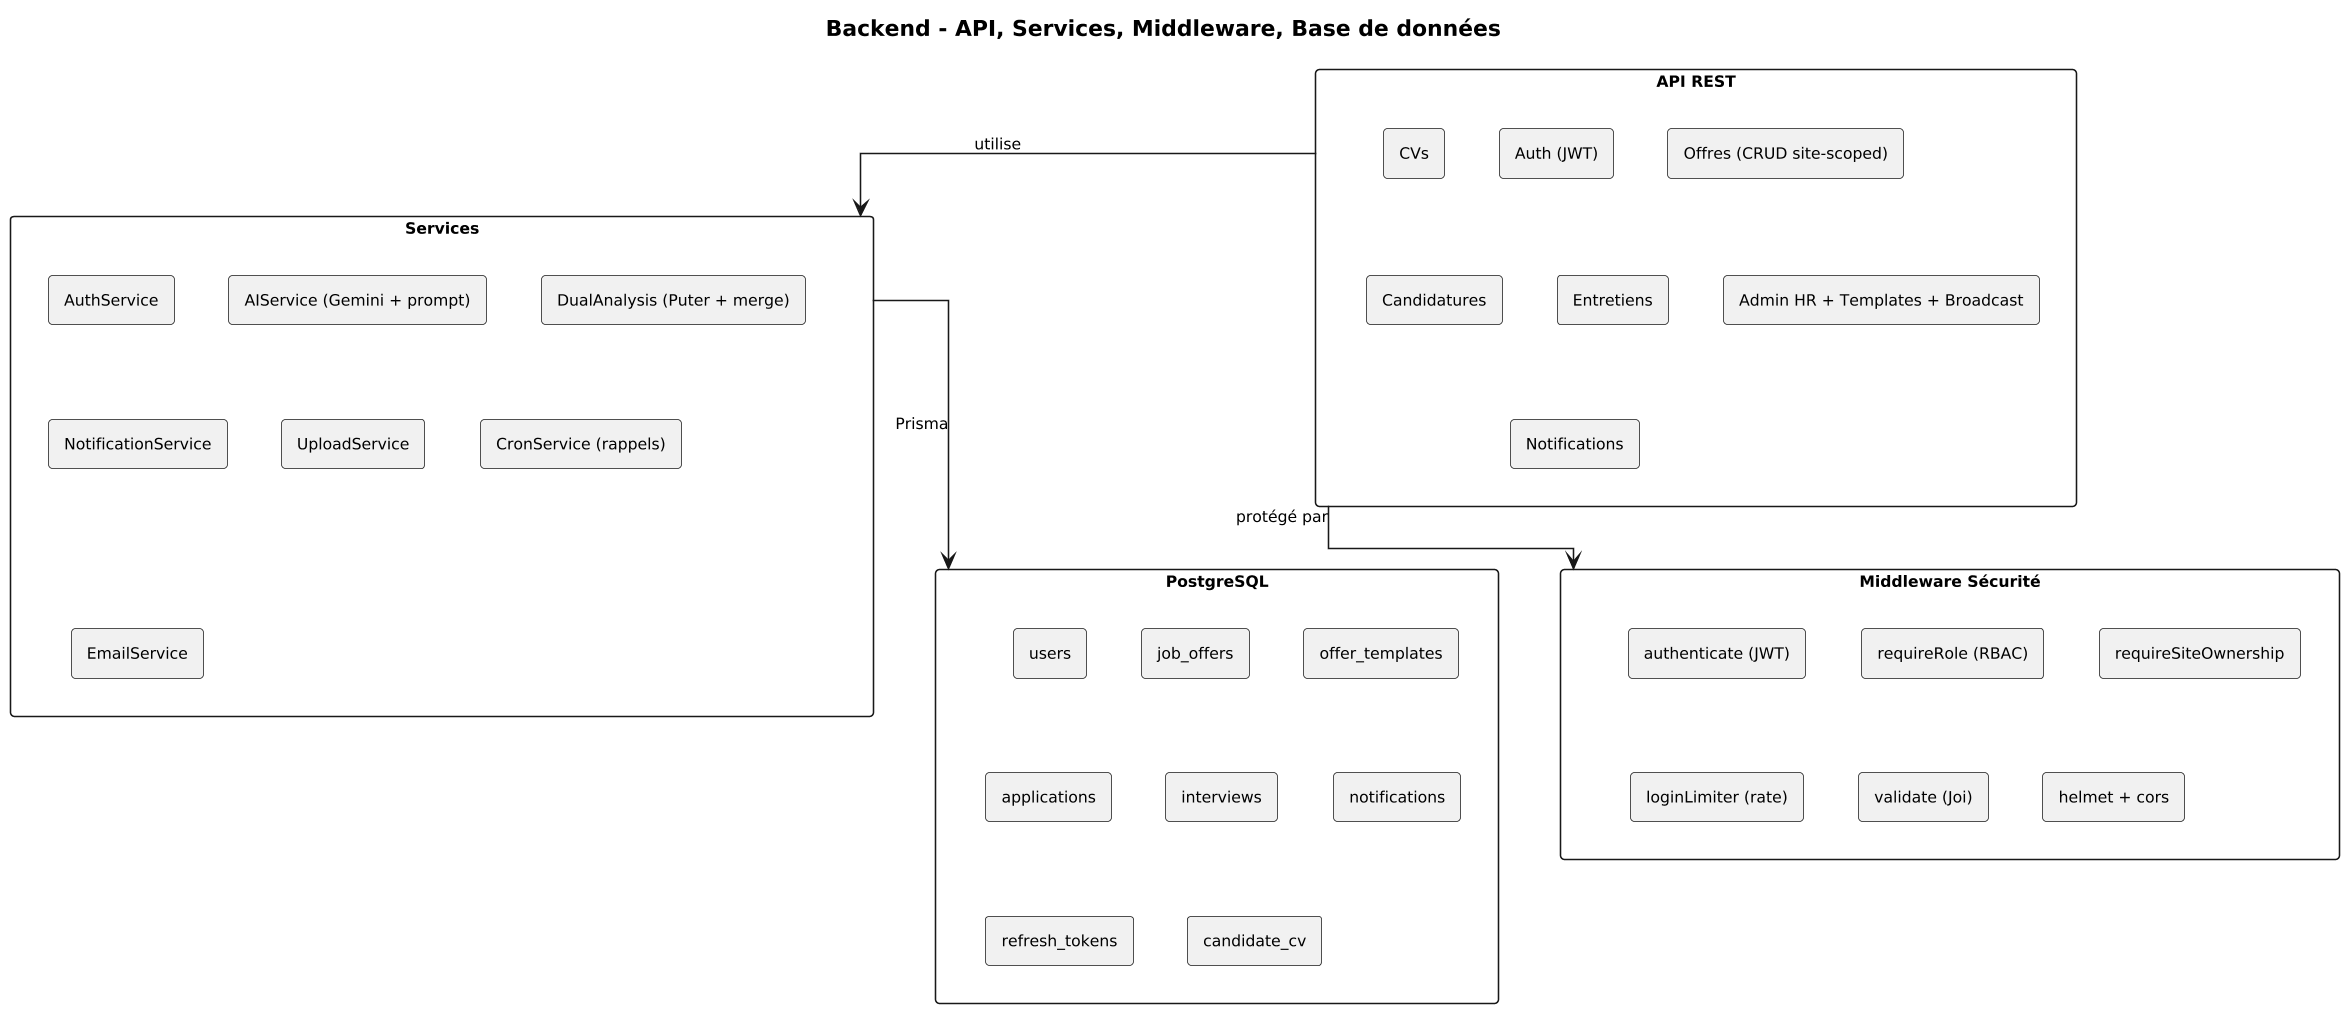
\includegraphics[width=\textwidth]{architecture_backend.png}
\caption{Architecture du backend Node.js/Express}
\end{figure}

Le backend concentre l'autorisation, la validation metier et l'orchestration des traitements asynchrones (analyse IA, notifications, rappels).

Cette couche centralise aussi des protections transverses: normalisation des statuts entrants (\texttt{review -> reviewing}), verification role/site/propriete sur les routes sensibles, limitation des mises a jour en lot, et validation de formats (date entretien, payload analyse). La centralisation evite des ecarts de comportement entre interfaces RH, admin et candidat.

\begin{figure}[H]
\centering
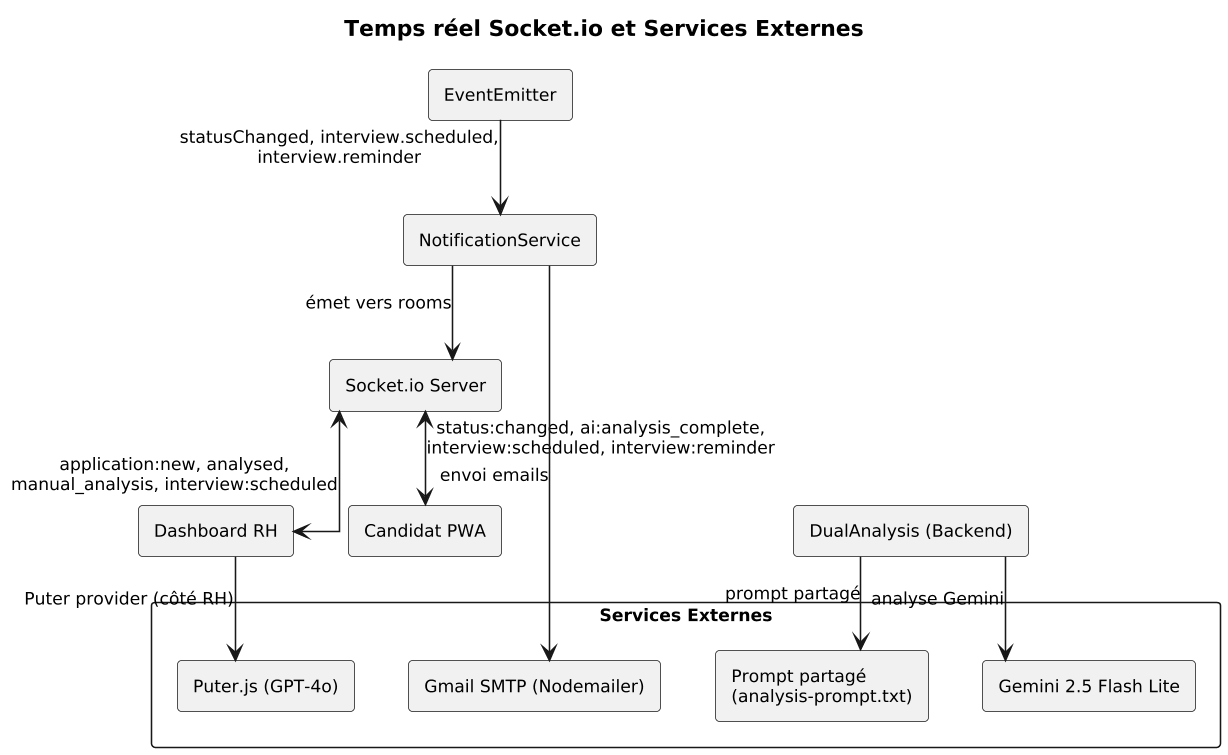
\includegraphics[width=\textwidth]{architecture_temps_reel_socket_services_externes.png}
\caption{Architecture temps reel et services externes}
\end{figure}

Le schema detaille les flux Socket.io (\texttt{status:changed}, \texttt{interview:scheduled}, \texttt{interview:reminder}) et les integrations externes (Gemini, Puter.js, SMTP).

L'implementation Socket repose sur des rooms a granularite metier: \texttt{user:\{id\}}, \texttt{candidate:\{id\}}, \texttt{hr:\{id\}}, \texttt{site:\{site\}} et \texttt{admin}. La connexion est authentifiee par JWT des le handshake; un jeton invalide bloque l'ouverture du canal. Ce choix limite les broadcasts globaux et reduit le risque de diffusion d'evenements hors perimetre.

\subsection{Principes retenus}

Quatre principes structurent la conception: regles metier centralisees cote API, separation stricte des couches, isolation des donnees par site, et traitement asynchrone pour les operations longues.

\section{Conception dynamique du processus de recrutement}

\subsection{Parcours candidat}

\begin{figure}[H]
\centering
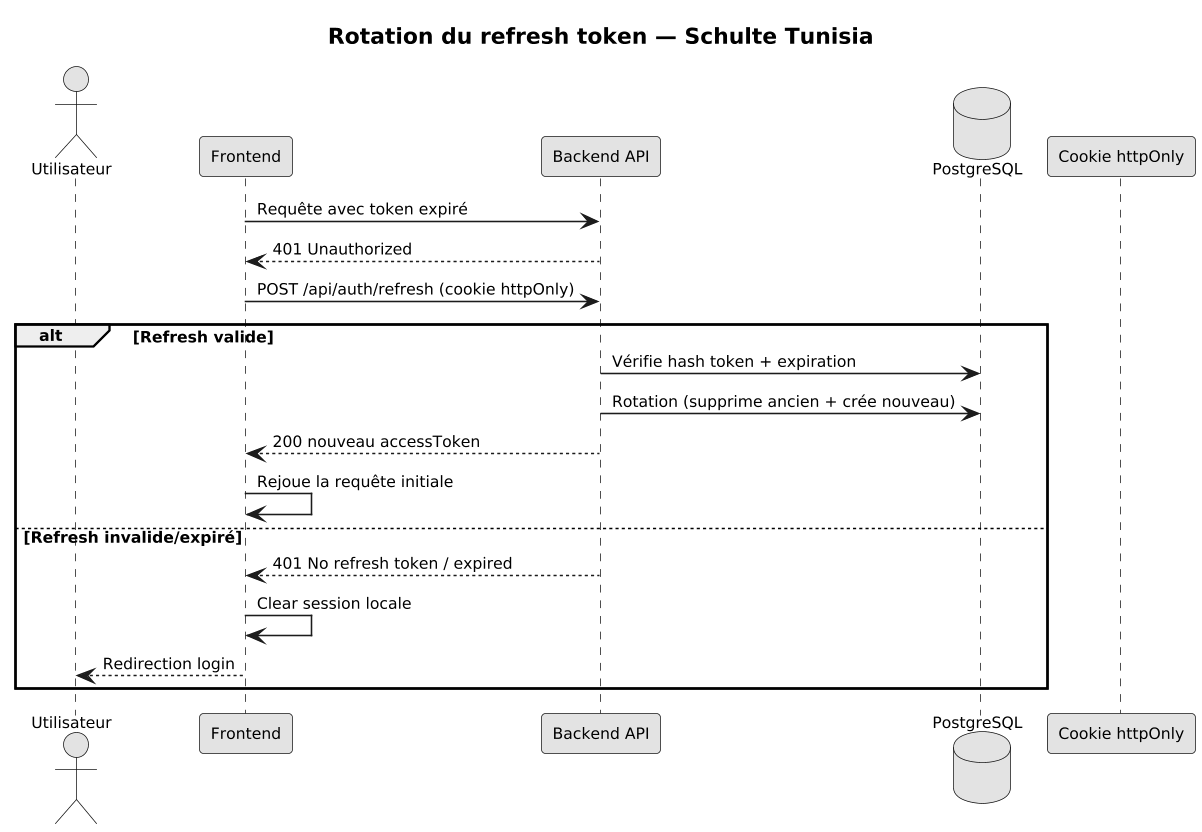
\includegraphics[width=\textwidth]{inscription_candidat.png}
\caption{Sequence d'inscription candidat}
\end{figure}

Ce diagramme decrit la creation de compte et les validations prealables a l'activation.

\begin{figure}[H]
\centering
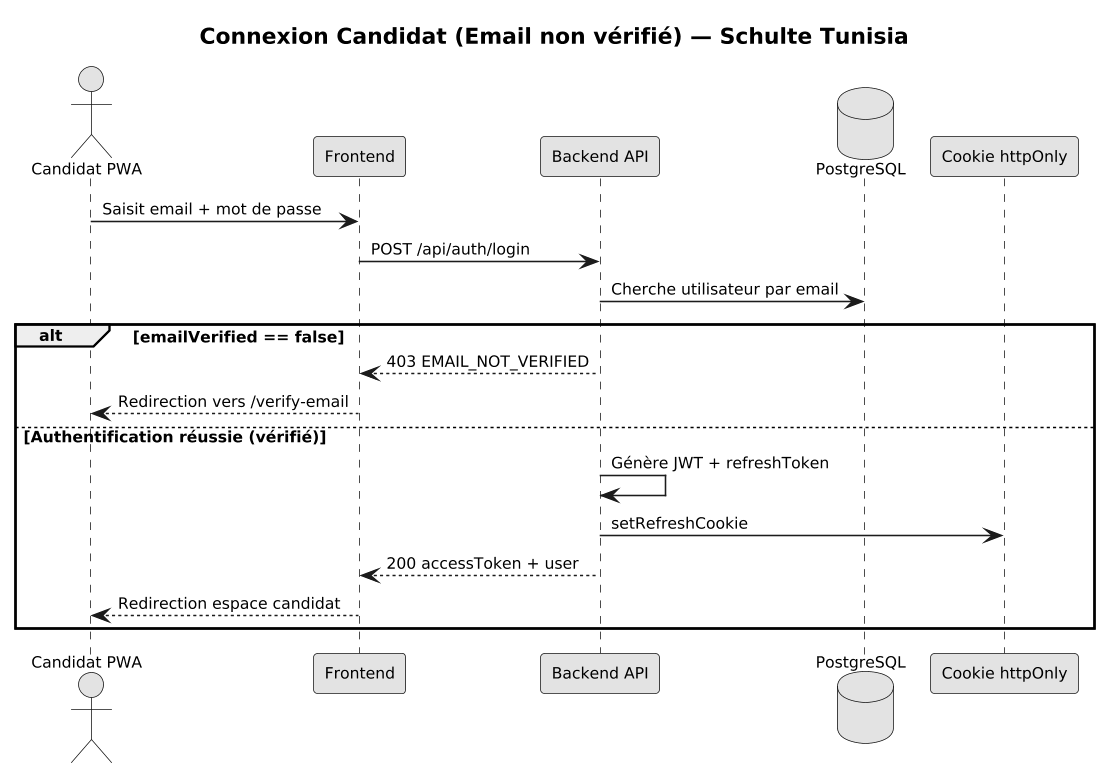
\includegraphics[width=\textwidth]{tentative_connexion_avant_verification.png}
\caption{Tentative de connexion avant verification email}
\end{figure}

Le flux de connexion avant verification montre le blocage volontaire de l'acces tant que l'email n'est pas confirme.

\begin{figure}[H]
\centering
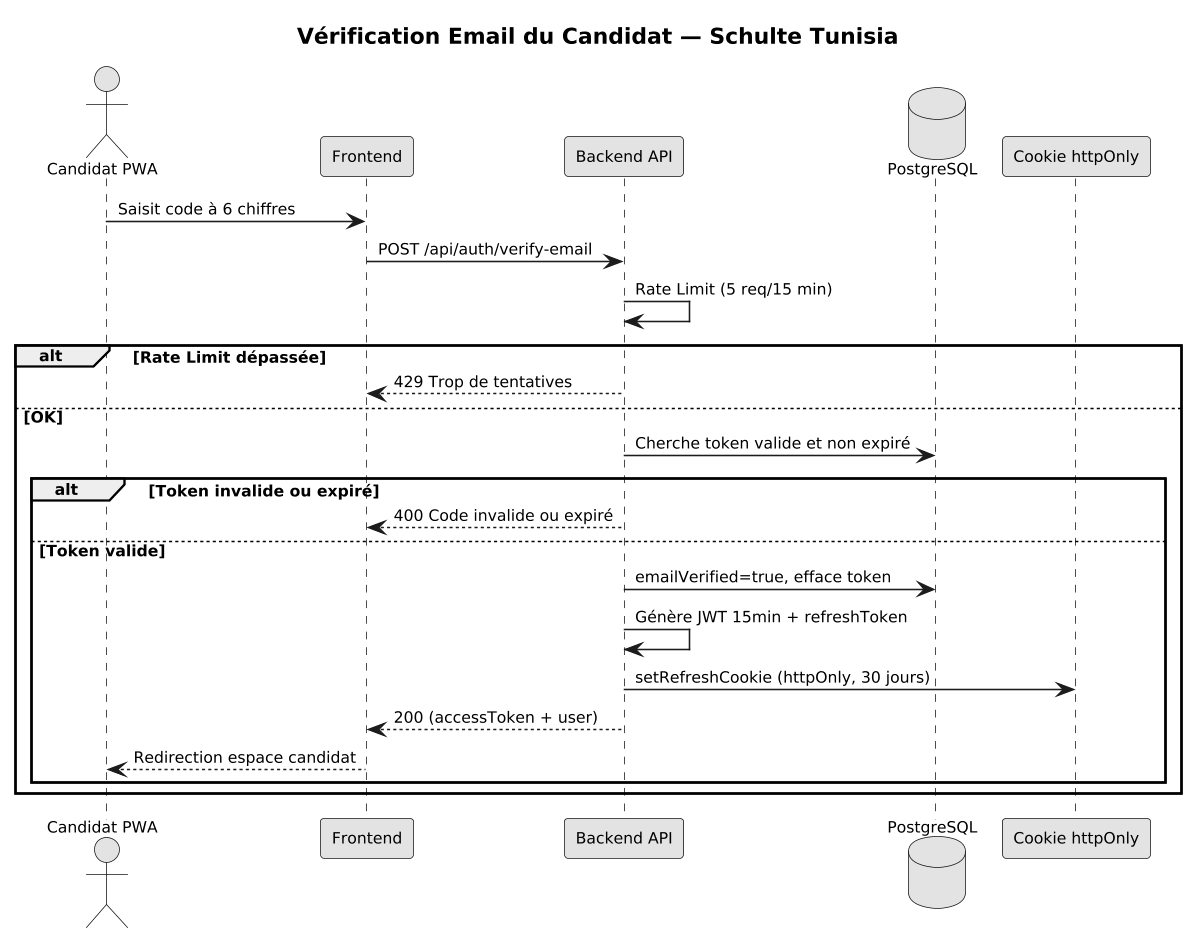
\includegraphics[width=\textwidth]{verification_email_premiere_connexion.png}
\caption{Verification email et premiere connexion}
\end{figure}

Cette etape ferme la boucle d'activation du compte candidat.

\begin{figure}[H]
\centering
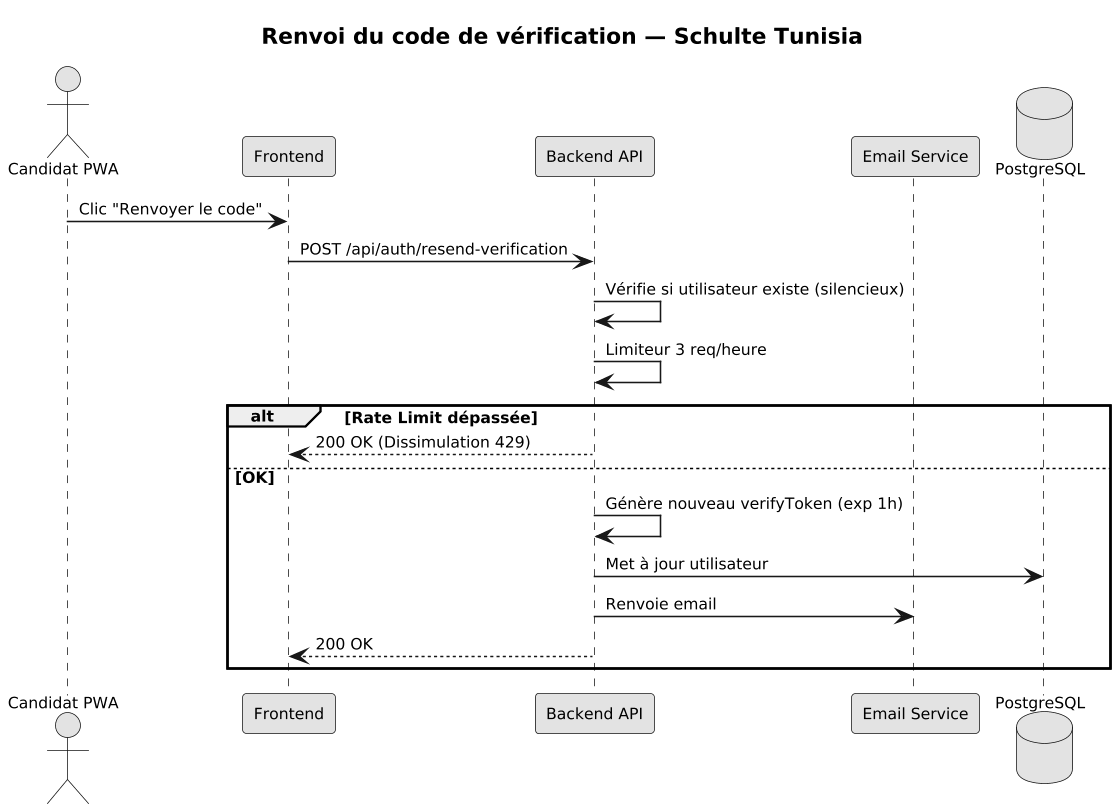
\includegraphics[width=\textwidth]{renvoi_code_verification.png}
\caption{Renvoi du code de verification}
\end{figure}

Le renvoi de code limite la perte de candidatures quand le mail de verification n'est pas recu ou expire.

\begin{figure}[H]
\centering
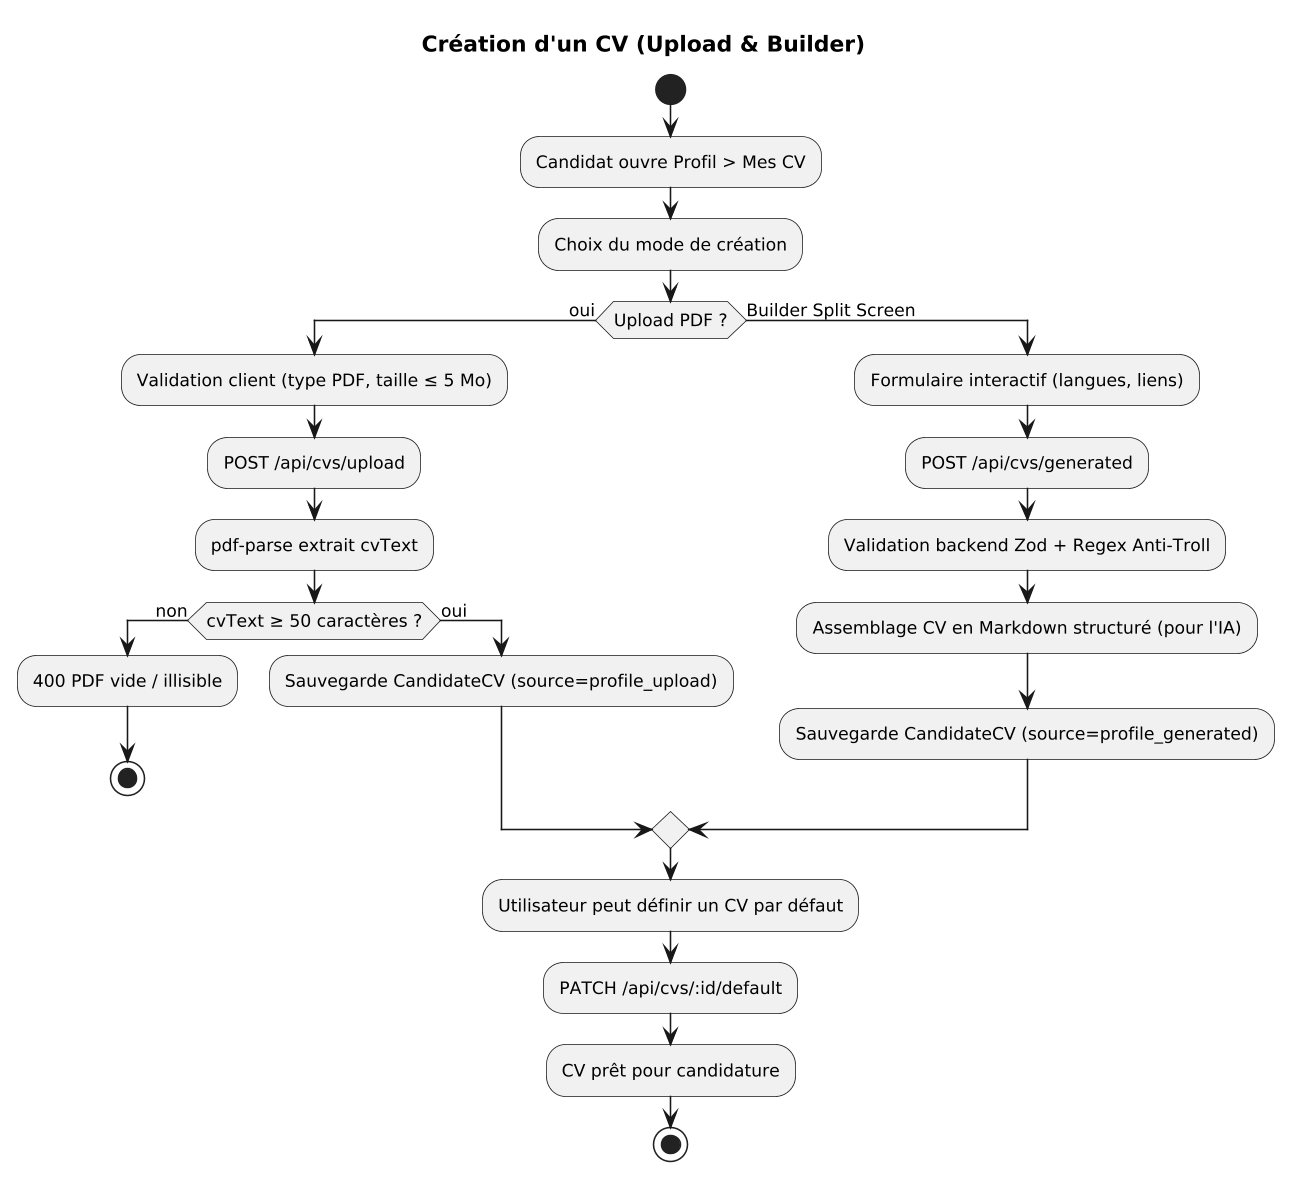
\includegraphics[width=\textwidth]{creation_cv_upload_builder.png}
\caption{Creation d'un CV (upload PDF ou formulaire)}
\end{figure}

Le candidat peut importer un CV PDF ou produire un CV via le builder. Les validations client et serveur reduisent les dossiers incomplets.

\begin{figure}[H]
\centering
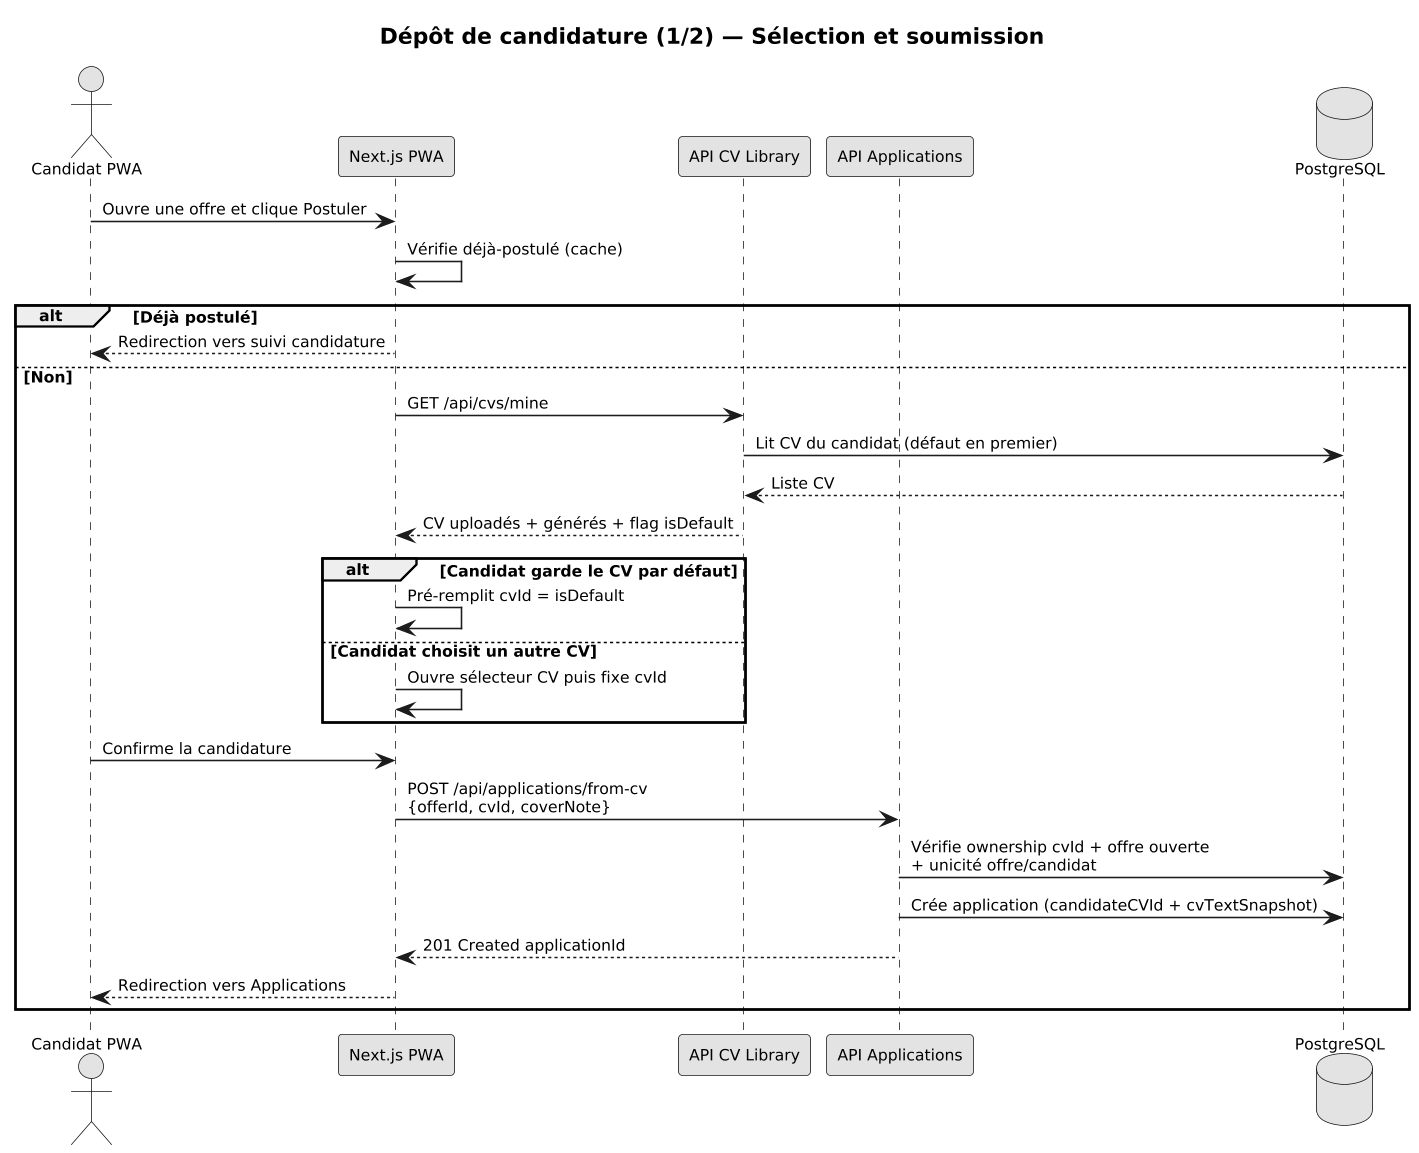
\includegraphics[width=\textwidth]{selection_cv_soumission_candidature.png}
\caption{Selection du CV puis soumission}
\end{figure}

Le choix du CV a ete separe de la soumission pour limiter les erreurs de dossier.

\begin{figure}[H]
\centering
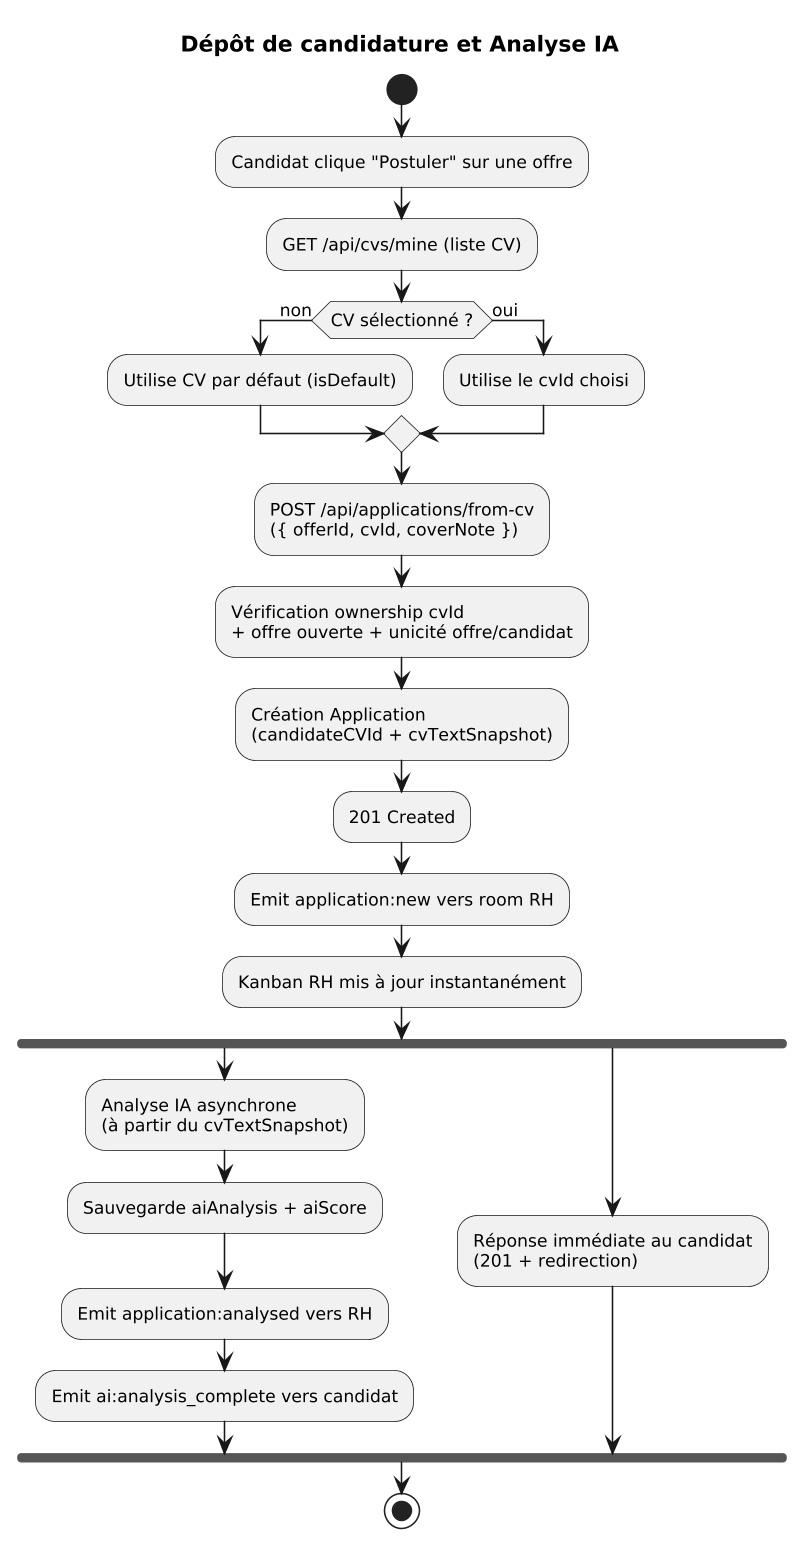
\includegraphics[width=\textwidth]{depot_candidature_analyse_ia.png}
\caption{Depot de candidature et lancement de l'analyse IA}
\end{figure}

La candidature est enregistree immediatement (\texttt{201 Created}) ; l'analyse IA continue ensuite en arriere-plan.

Au moment du depot, le texte CV est fige dans un instantane (\texttt{cvTextSnapshot}) pour decoupler l'analyse du contenu evolutif de la bibliotheque CV. Cette decision garantit la reproductibilite: une meme candidature est evaluee sur la meme base textuelle, meme si le candidat modifie son CV apres soumission.

\subsection{Orchestration de l'analyse IA}

\begin{figure}[H]
\centering
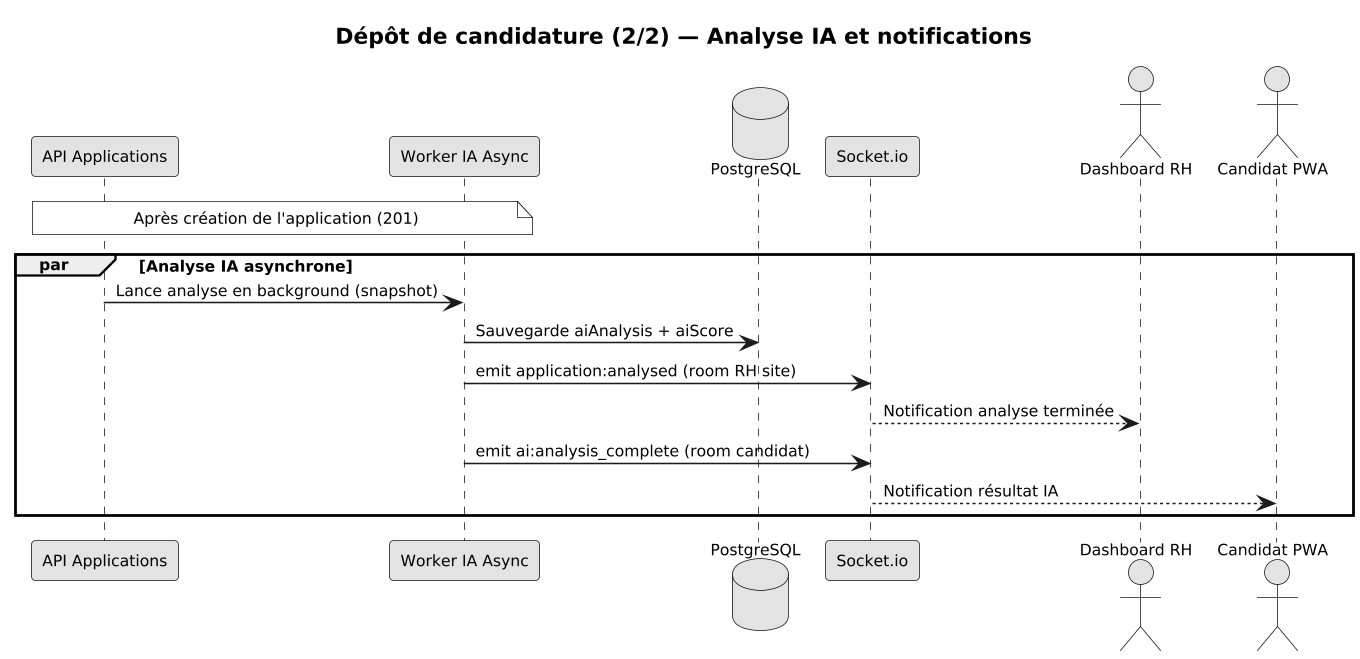
\includegraphics[width=\textwidth]{analyse_ia_async_notifications_socket.png}
\caption{Analyse IA asynchrone et notification temps reel}
\end{figure}

Ce flux montre le decouplage entre depot de candidature et calcul IA, puis la notification automatique du RH.

\begin{figure}[H]
\centering
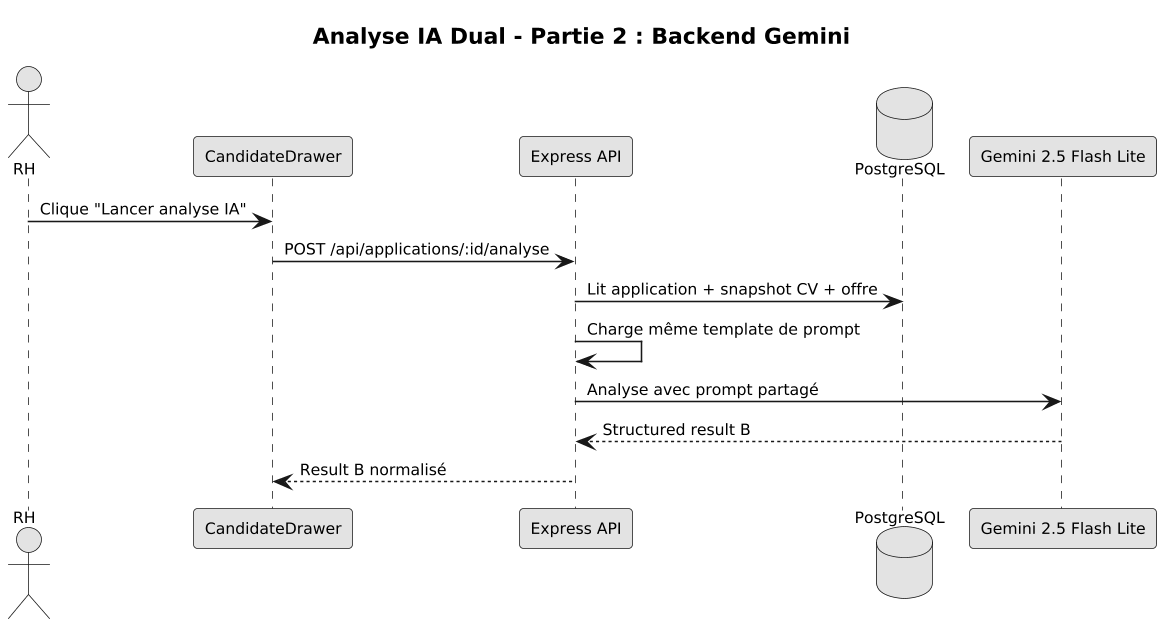
\includegraphics[width=\textwidth]{analyse_backend_gemini.png}
\caption{Analyse IA cote backend (Gemini)}
\end{figure}

Le backend produit une premiere evaluation standardisee a partir du meme prompt partage.

\begin{figure}[H]
\centering
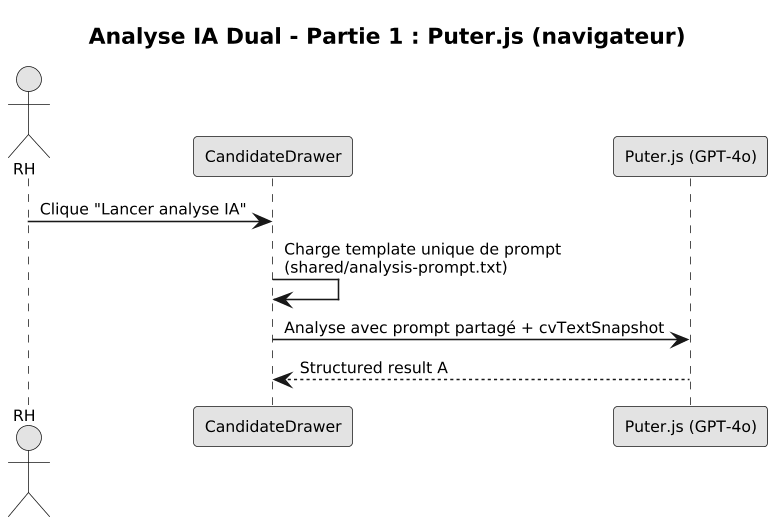
\includegraphics[width=\textwidth]{analyse_puterjs.png}
\caption{Analyse IA cote navigateur RH (Puter.js)}
\end{figure}

La voie Puter.js permet une relecture dynamique au moment de l'examen RH, sans bloquer le depot initial.

Le module RH de double analyse applique des gardes techniques explicites: nettoyage des sorties IA (\texttt{parseRawJSON}) pour retirer les enveloppes Markdown, parsing tolerant des anciens formats stockes, et fallback backend si Puter.js est indisponible. Si une analyse backend valide est deja presente dans \texttt{aiAnalysis}, elle est rehydratee pour eviter des appels externes inutiles.

\begin{figure}[H]
\centering
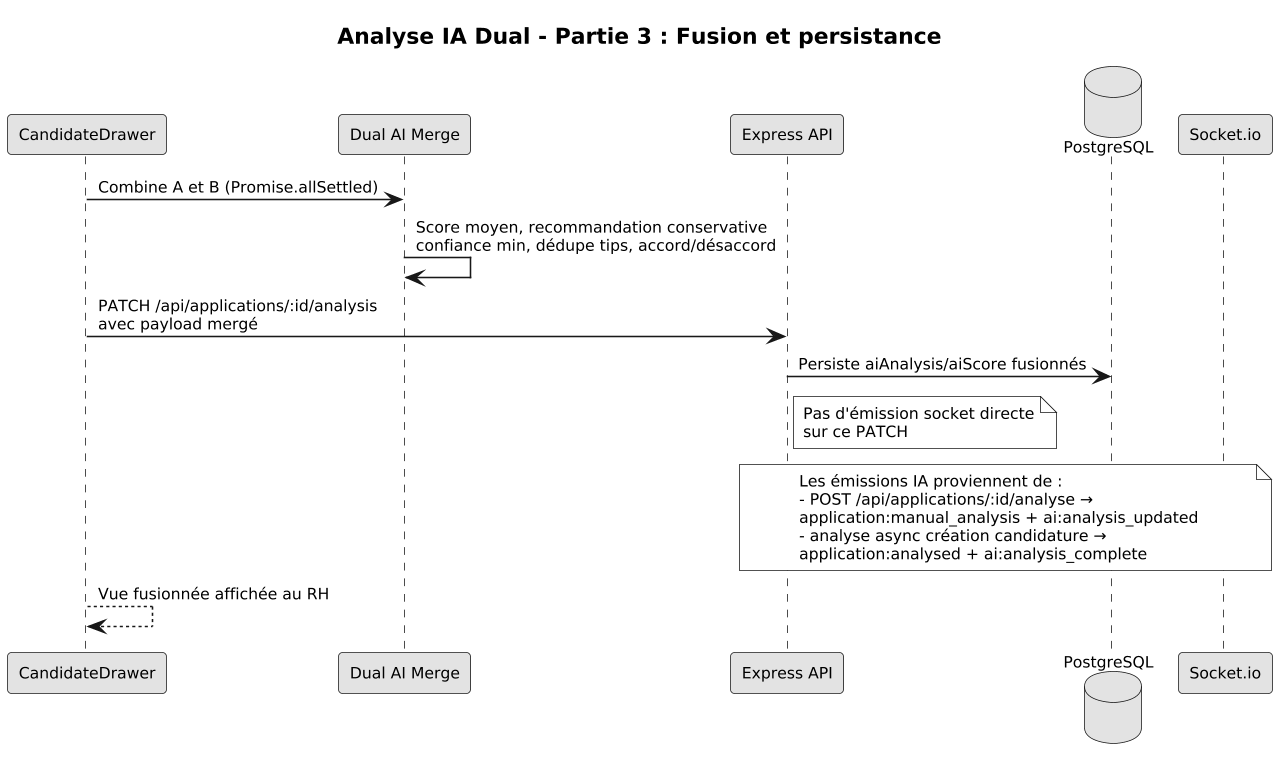
\includegraphics[width=\textwidth]{fusion_resultats_persistance.png}
\caption{Fusion des resultats IA et persistance}
\end{figure}

Les sorties IA sont fusionnees (score moyen, recommandation prudente) pour produire un resultat exploitable et trace.

La fusion applique une logique conservative sur la recommandation: en cas de divergence, l'ordre de priorite retenu est \texttt{Reject < Request More Info < Interview < Hire}. Cette regle minimise les faux positifs et preserve une marge de decision humaine sur les dossiers ambigus.

\begin{figure}[H]
\centering
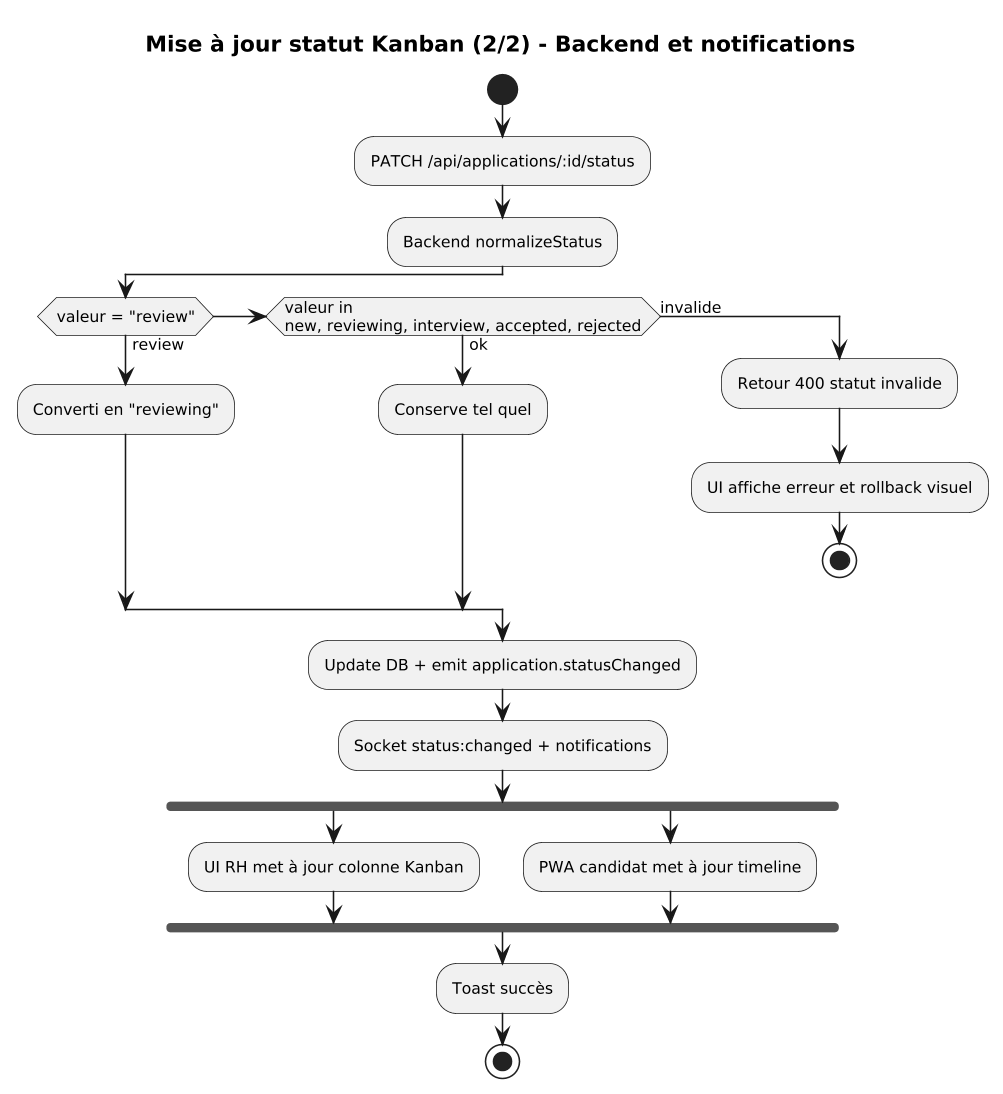
\includegraphics[width=\textwidth]{mise_a_jour_backend_normalisation_notifications.png}
\caption{Normalisation backend et diffusion des mises a jour}
\end{figure}

Le backend normalise les donnees (ex. conversion des statuts UI) puis notifie les clients concernes en temps reel.

\subsection{Cycle RH et entretien}

\begin{figure}[H]
\centering
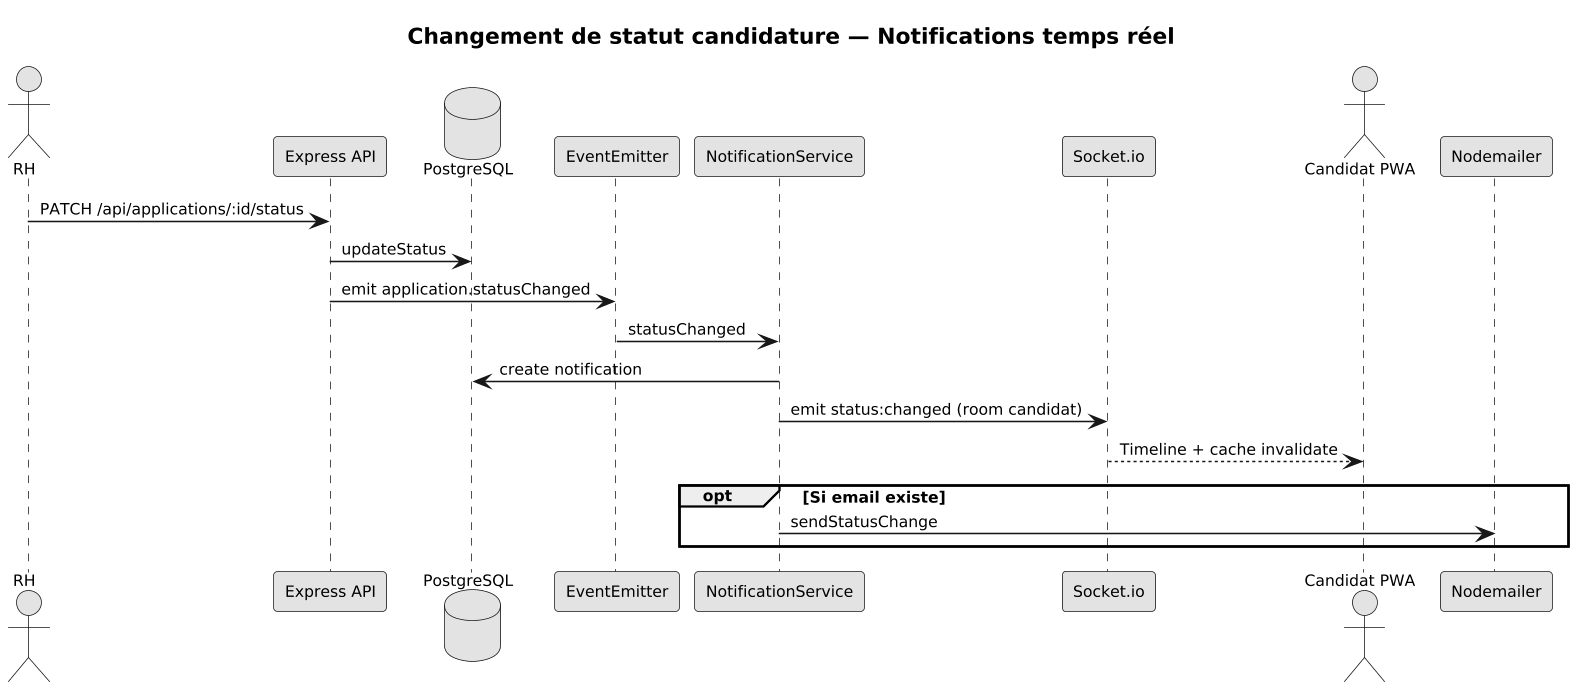
\includegraphics[width=\textwidth]{changement_statut_candidature.png}
\caption{Flux de changement de statut d'une candidature}
\end{figure}

Ce diagramme formalise les transitions autorisees dans le Kanban RH.

\begin{figure}[H]
\centering
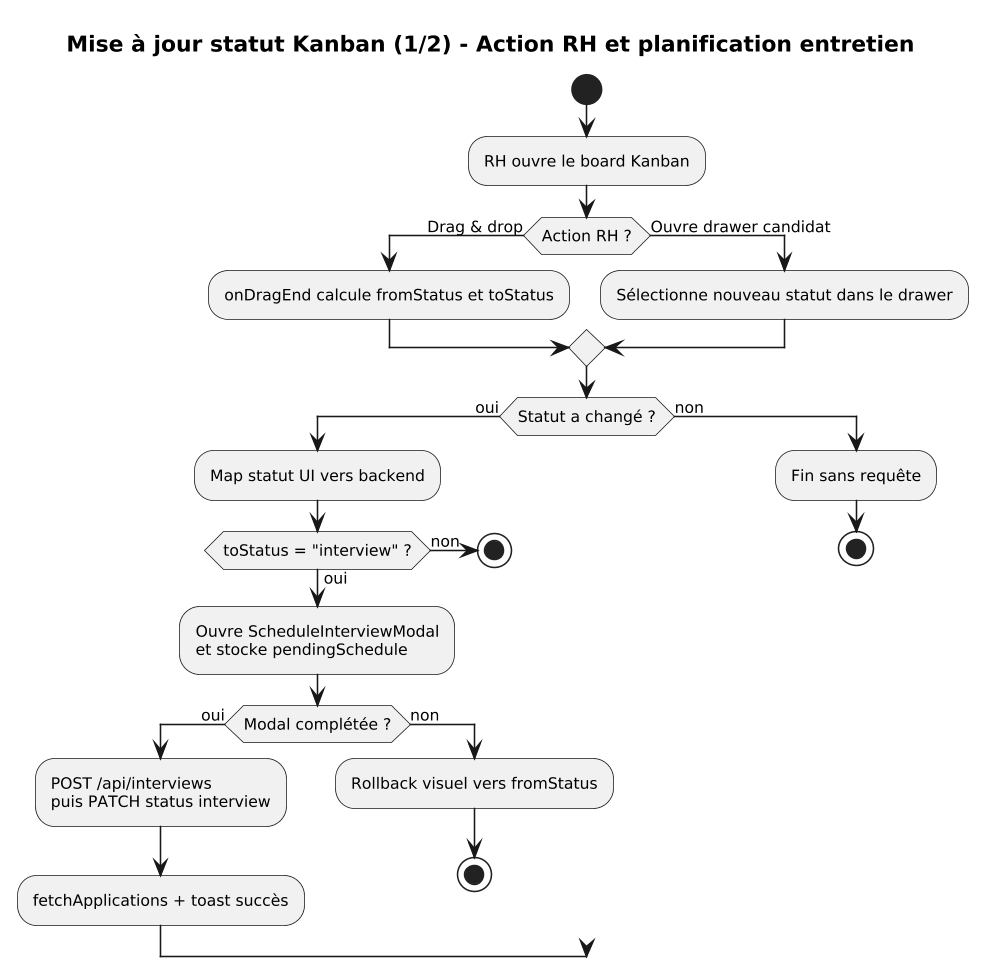
\includegraphics[width=\textwidth]{action_rh_planification_statut_interview.png}
\caption{Action RH et declenchement de planification}
\end{figure}

La planification n'est autorisee qu'apres passage dans l'etat approprie (\texttt{interview}).

La route de planification verifie aussi des preconditions metier strictes: date valide, appartenance site pour les RH, et blocage des candidatures deja finalisees (\texttt{accepted}/\texttt{rejected}). En cas de replanification, l'entretien existant est mis a jour et le drapeau \texttt{reminderSent} est reinitialise afin de relancer proprement le cycle de rappel.

\begin{figure}[H]
\centering
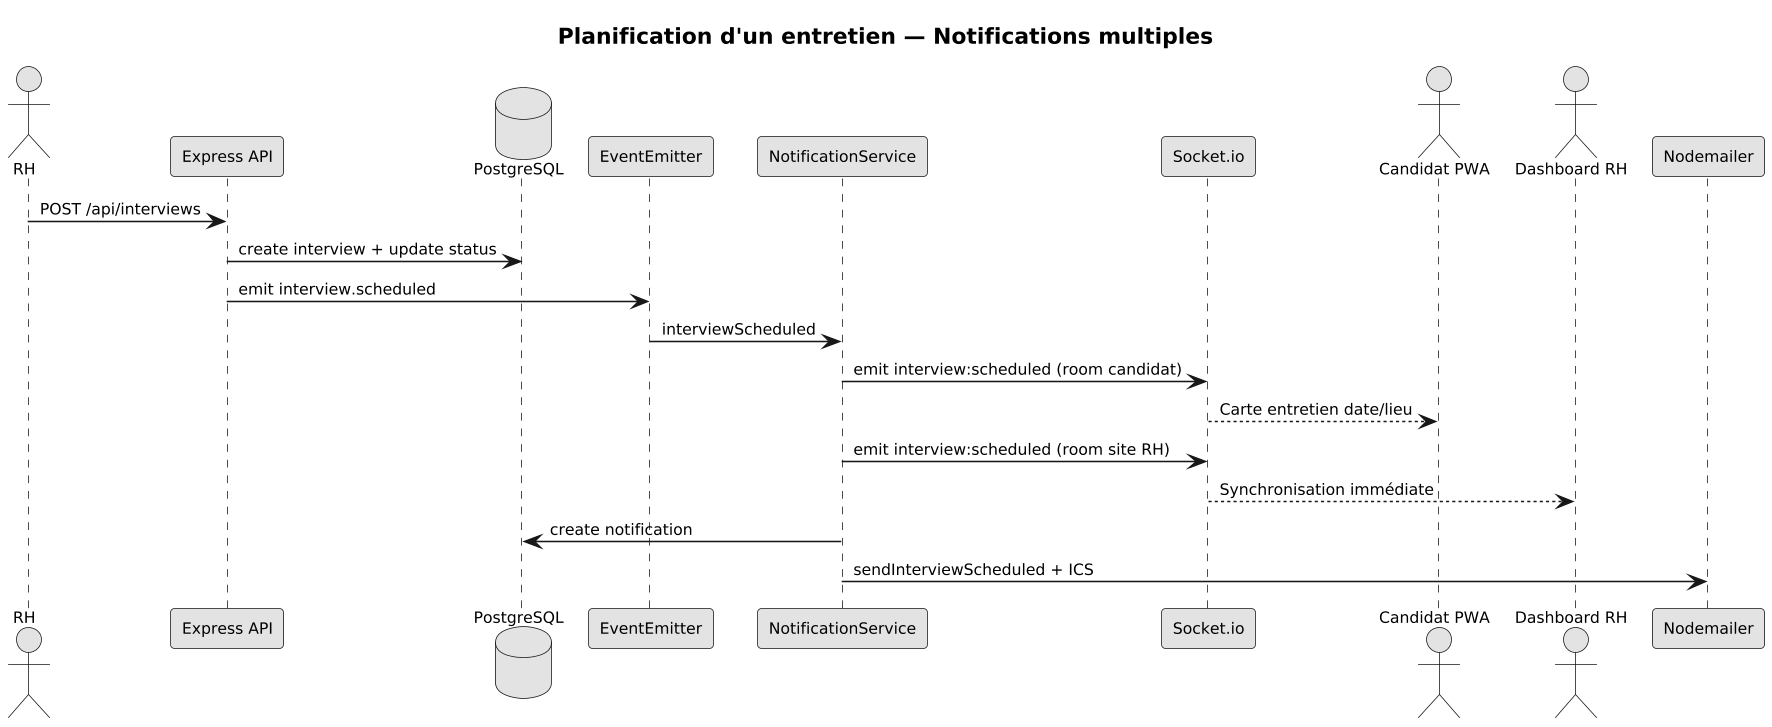
\includegraphics[width=\textwidth]{planification_entretien_initiale.png}
\caption{Planification initiale d'un entretien}
\end{figure}

Nous y decrivons la creation d'un rendez-vous avec ses contraintes de base (date, heure, lien ou salle, message).

\begin{figure}[H]
\centering
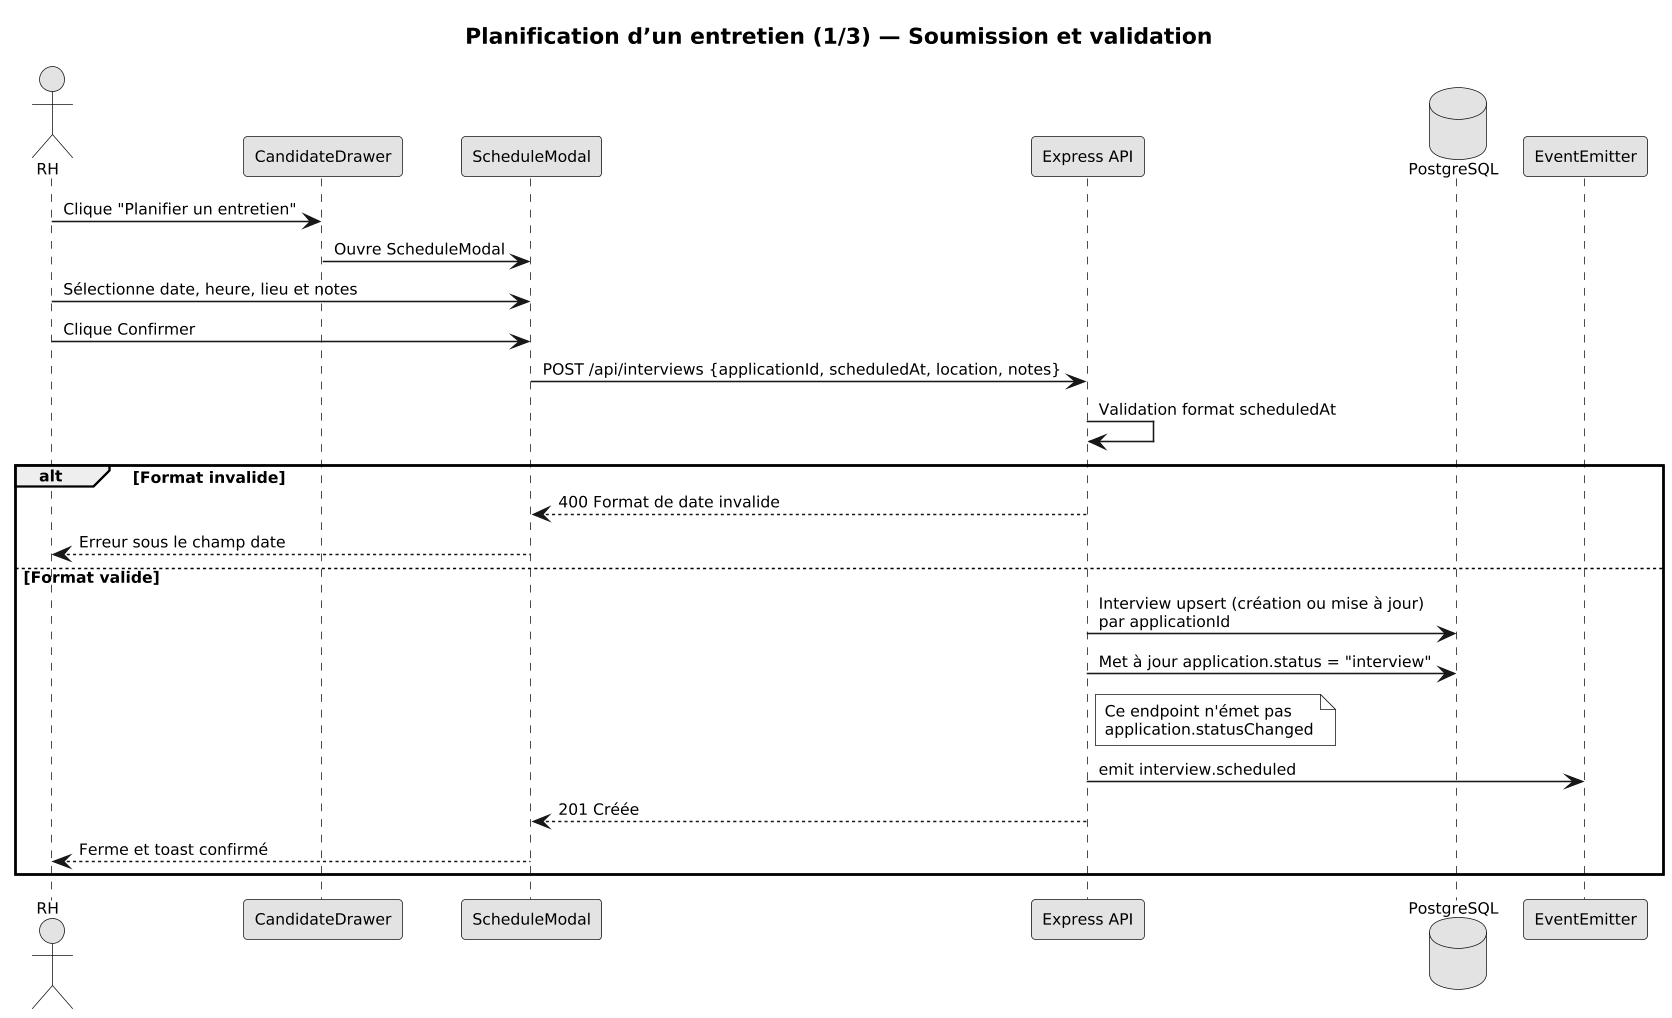
\includegraphics[width=\textwidth]{planification_entretien_maj.png}
\caption{Mise a jour ou replanification d'entretien}
\end{figure}

Le flux de replanification preserve l'historique pour garder la tracabilite.

\begin{figure}[H]
\centering
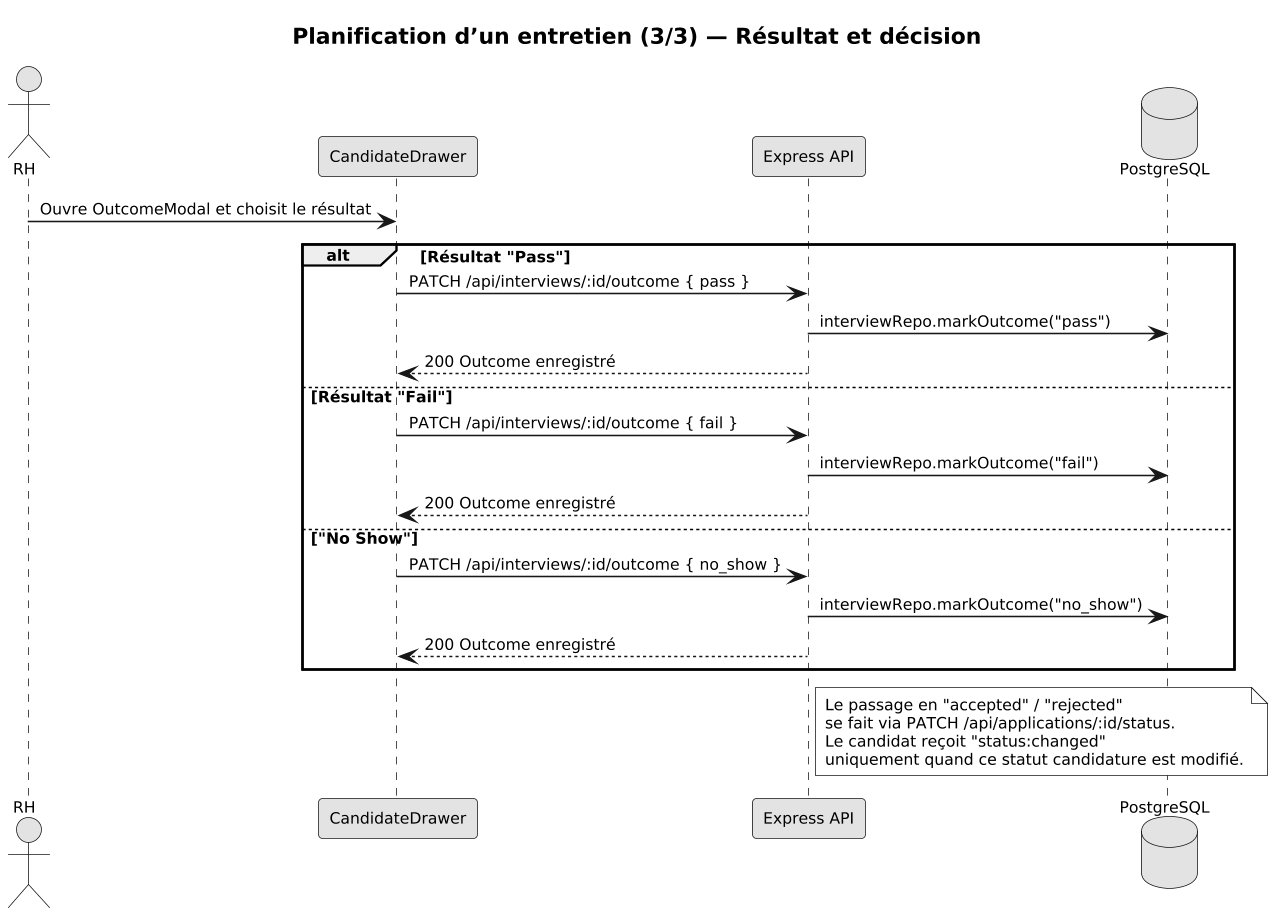
\includegraphics[width=\textwidth]{enregistrement_resultat_entretien.png}
\caption{Enregistrement du resultat d'entretien}
\end{figure}

La decision d'entretien (\texttt{pass}, \texttt{fail}, \texttt{no\_show}) alimente ensuite la transition vers les etats de fin.

\subsection{Machine a etats candidature}

\begin{figure}[H]
\centering
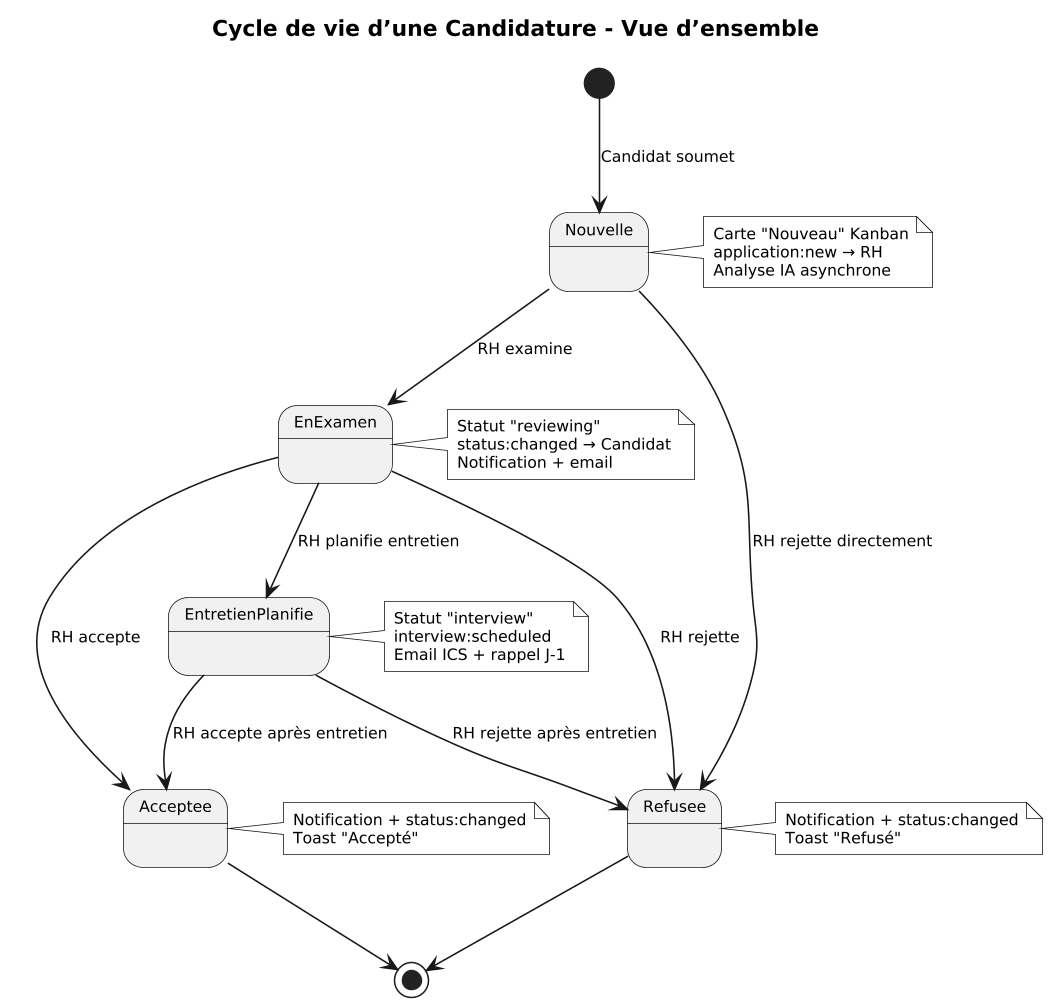
\includegraphics[width=\textwidth]{vue_ensemble_etats_principaux.png}
\caption{Vue d'ensemble des etats candidature}
\end{figure}

Le diagramme fixe le cycle complet, du statut initial aux statuts terminaux.

\begin{figure}[H]
\centering
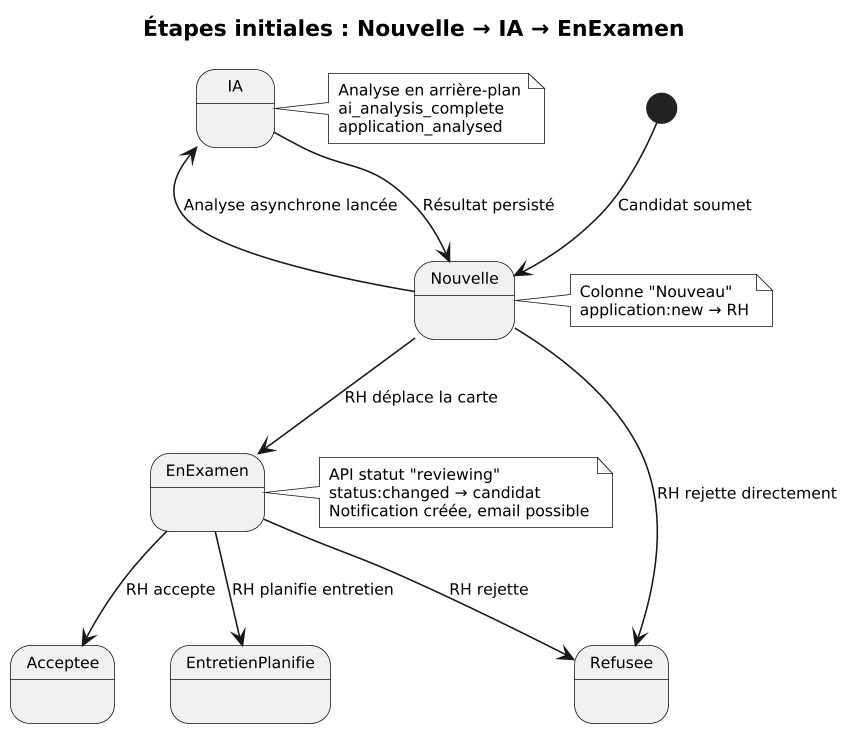
\includegraphics[width=\textwidth]{detail_etapes_initiales_nouvelle_ia_enexamen.png}
\caption{Detail des etapes initiales}
\end{figure}

Nous y precisons la progression controlee entre reception, analyse et examen RH (\texttt{new -> reviewing}).

\begin{figure}[H]
\centering
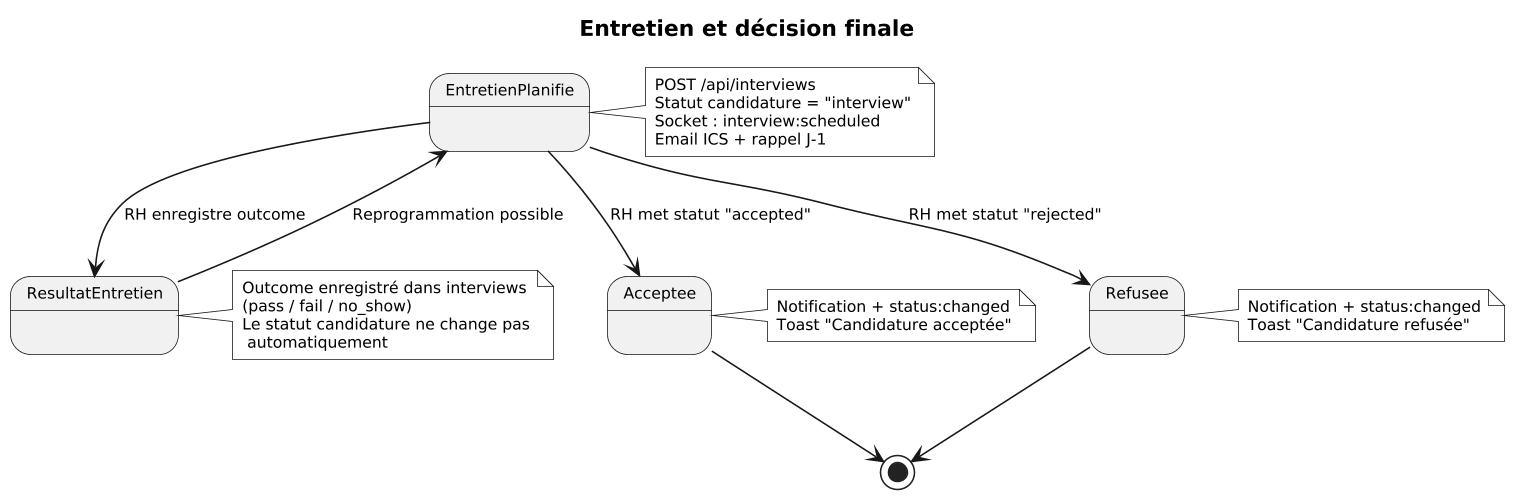
\includegraphics[width=\textwidth]{detail_etats_entretien_resultat_fin.png}
\caption{Detail des etats entretien et fin de cycle}
\end{figure}

Cette partie explicite les decisions finales et leur impact metier.

\begin{figure}[H]
\centering
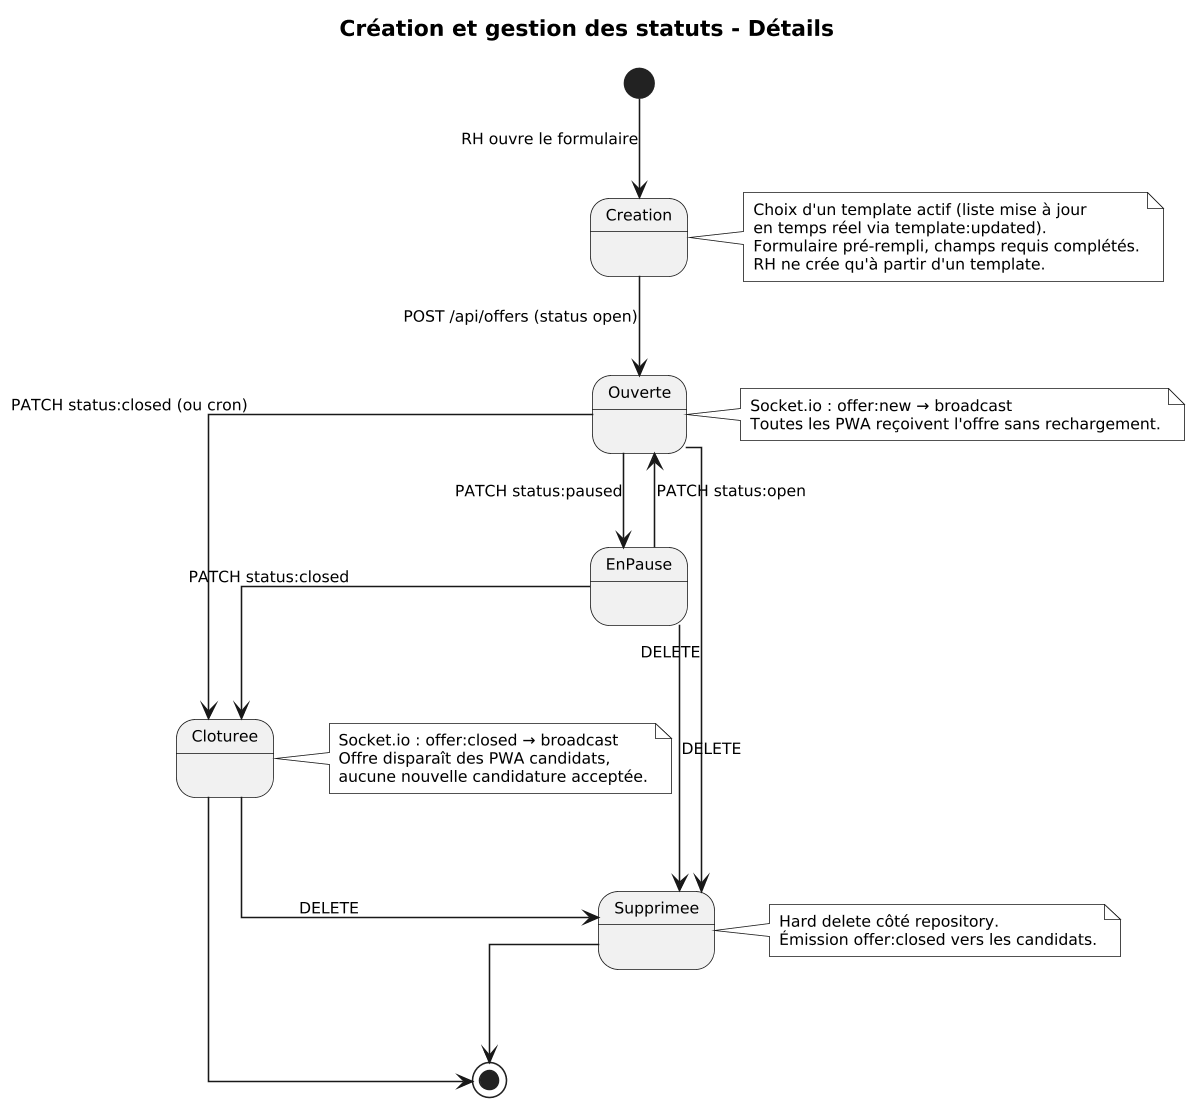
\includegraphics[width=\textwidth]{details_transitions_notifications.png}
\caption{Transitions d'etat et notifications associees}
\end{figure}

Chaque transition importante declenche une notification ciblee pour le bon acteur.

Pour la consultation RH/Admin, les entretiens sont exposes avec pagination par \texttt{limit} et \texttt{cursor} temporel (\texttt{scheduledAt}). Cette strategie limite les chargements volumineux et facilite un rafraichissement progressif des tableaux de suivi.

\subsection{Cas limites et scenarios d'erreur traites}

La conception dynamique a integre des cas limites reels observes dans le code applicatif, afin d'eviter des incoherences fonctionnelles en production. Le tableau suivant resume les protections principales.

\begin{table}[H]
\centering
\caption{Cas limites integres a la conception dynamique}
\begin{tabularx}{\textwidth}{|l|X|X|}
\hline
\textbf{Cas limite} & \textbf{Regle de conception} & \textbf{Comportement attendu} \\
\hline
Acces RH hors site sur candidature ou entretien & Verification role + site avant lecture/modification & Rejet explicite en \texttt{403} (interdiction inter-site). \\
\hline
Planification d'entretien sur dossier deja finalise & Blocage des statuts terminaux \texttt{accepted}/\texttt{rejected} & Rejet metier en \texttt{409} pour eviter une reouverture implicite. \\
\hline
Soumission de candidature en doublon & Unicite candidat/offre verifiee avant creation & Rejet en \texttt{409} avec message de doublon. \\
\hline
Mise a jour de statut en lot non maitrisee & Limite de taille de lot + transaction atomique & Rejet au dela du seuil; sinon mise a jour coherente de tout le lot. \\
\hline
CV insuffisant ou invalide & Validation de contenu (taille texte, structure formulaire) & Rejet en \texttt{400} avant persistance d'une candidature exploitable. \\
\hline
\end{tabularx}
\end{table}

\section{Conception de la securite}

\subsection{Authentification et cycle des jetons}

\begin{figure}[H]
\centering
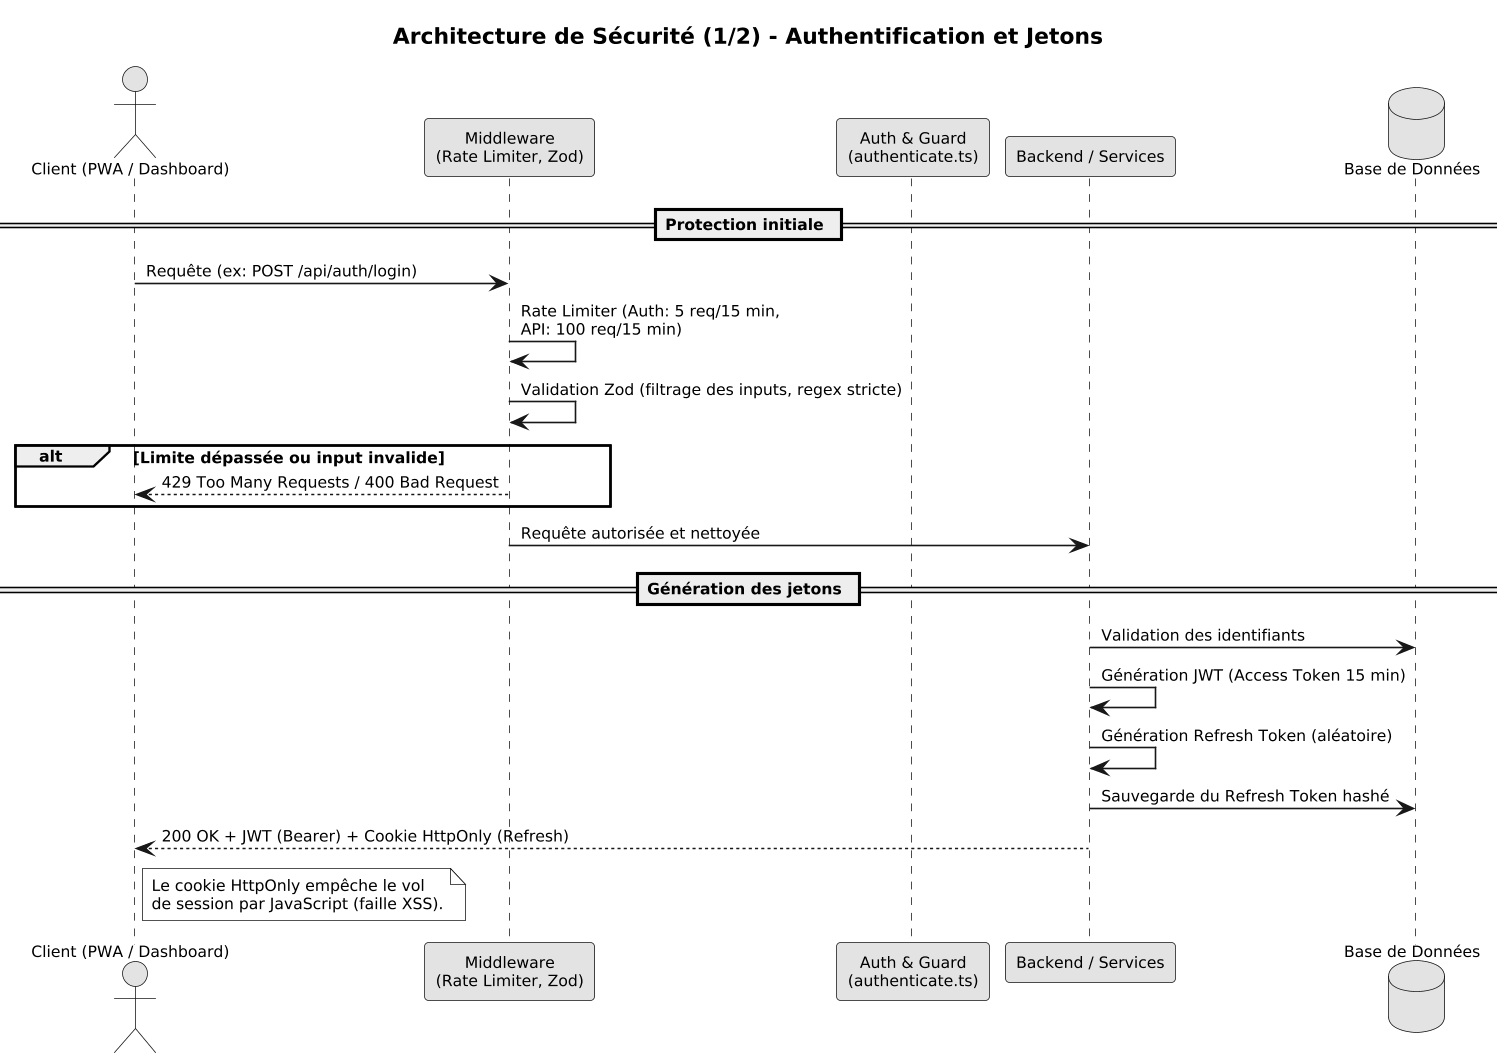
\includegraphics[width=\textwidth]{authentification_generation_jetons.png}
\caption{Authentification et generation des jetons}
\end{figure}

Ce diagramme presente l'emission du token d'acces et du refresh token.

\begin{figure}[H]
\centering
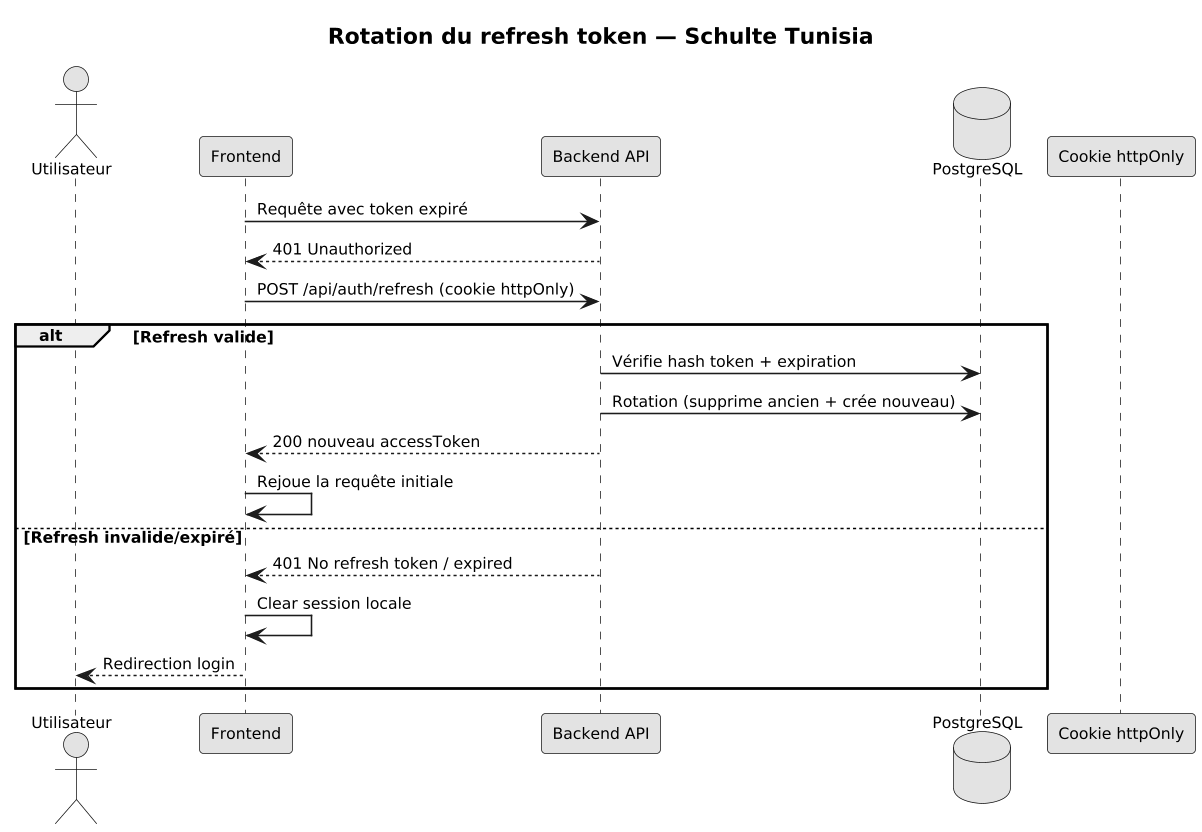
\includegraphics[width=\textwidth]{rotation_refresh_token.png}
\caption{Rotation du refresh token}
\end{figure}

La rotation limite l'impact d'un jeton compromis sur une longue duree.

\begin{figure}[H]
\centering
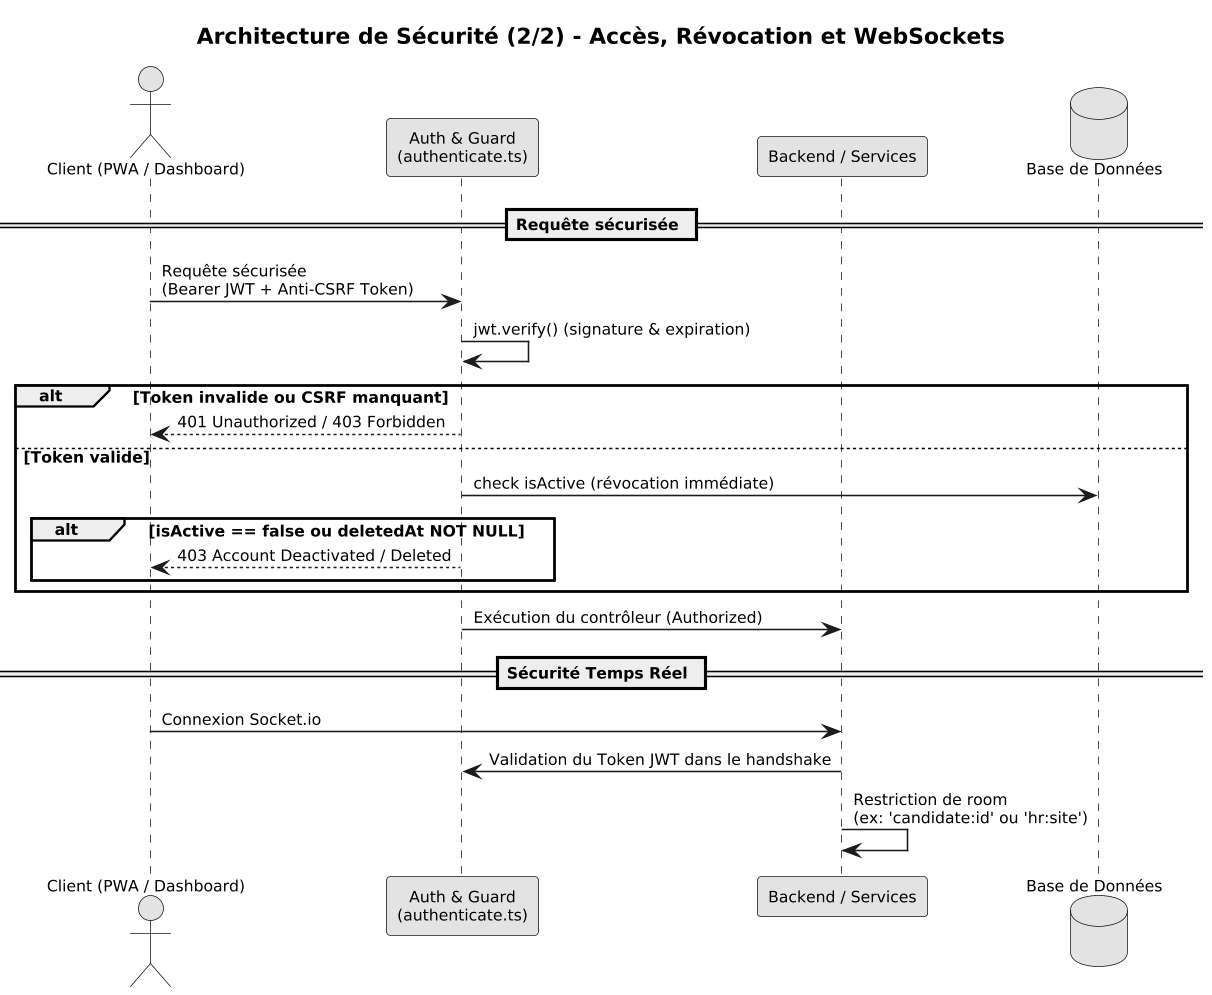
\includegraphics[width=\textwidth]{acces_securise_revocation_websockets.png}
\caption{Acces securise, revocation et controle WebSocket}
\end{figure}

Nous appliquons le meme principe de controle sur HTTP et WebSocket: verification du jeton, revocation immediate des comptes inactifs, et diffusion ciblee selon le role et le site. Le mecanisme de session repose sur un acces token court et un refresh token en rotation, avec invalidation de l'ancien jeton apres renouvellement.

Le refresh token n'est pas stocke en clair: seule une empreinte SHA-256 est persistee en base. Cote navigateur, il est place en cookie \texttt{HttpOnly}, borne au chemin \texttt{/api/auth/refresh}, avec \texttt{sameSite=lax} et \texttt{secure} en production. Ce parametrage reduit les risques d'exfiltration JavaScript et restreint l'usage du cookie au seul endpoint de renouvellement.

\subsection{Comportements de securite applicative}

\begin{figure}[H]
\centering
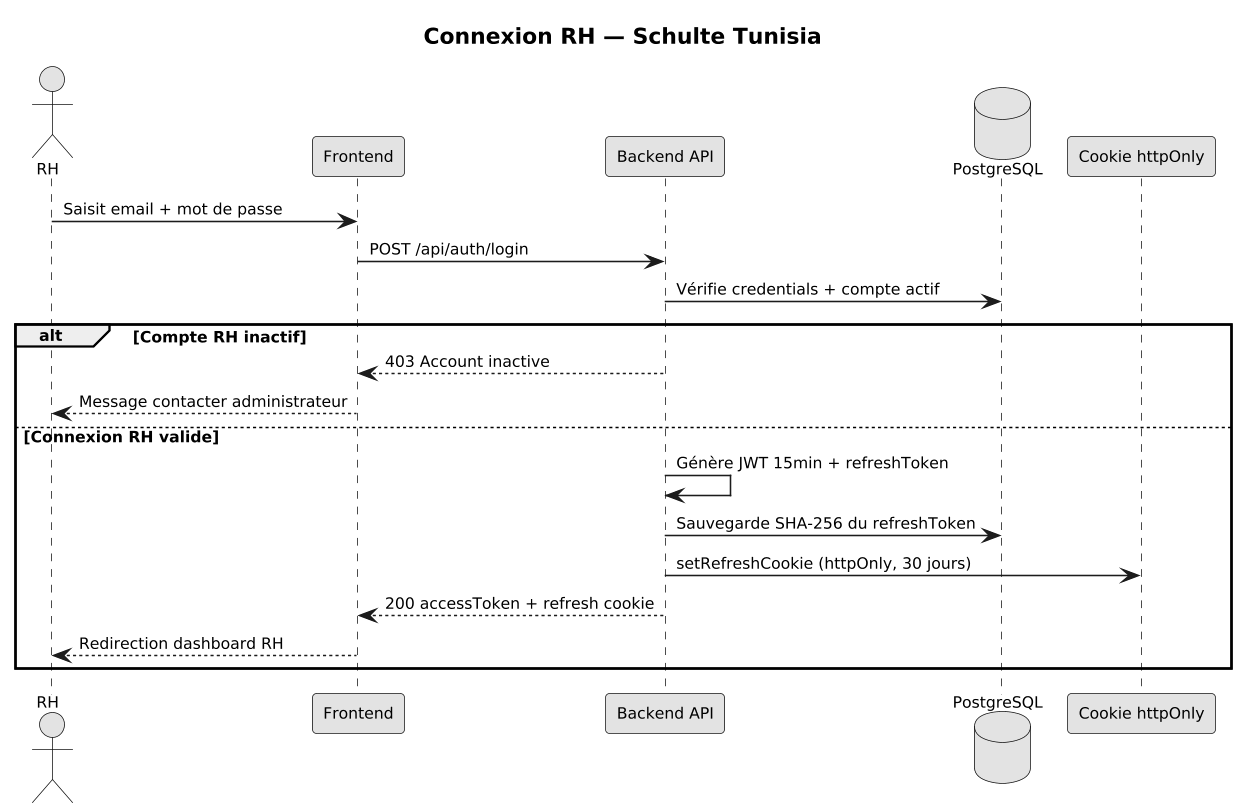
\includegraphics[width=\textwidth]{connexion_rh.png}
\caption{Connexion RH}
\end{figure}

Le flux RH inclut verification de role et perimetre de site.

\begin{figure}[H]
\centering
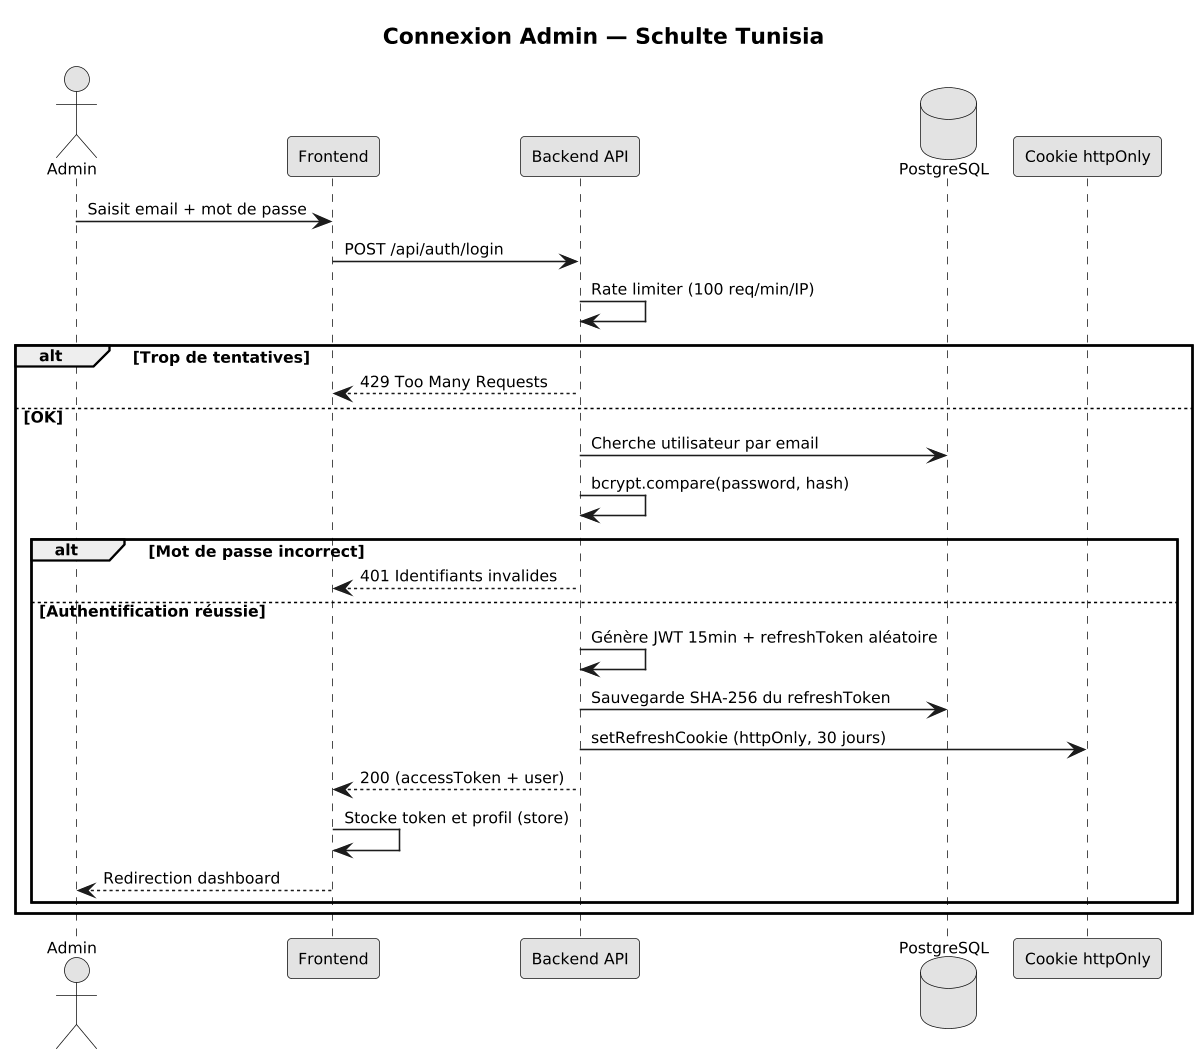
\includegraphics[width=\textwidth]{connexion_admin.png}
\caption{Connexion Admin}
\end{figure}

Le flux admin separe les privileges de gouvernance des operations RH.

\begin{figure}[H]
\centering
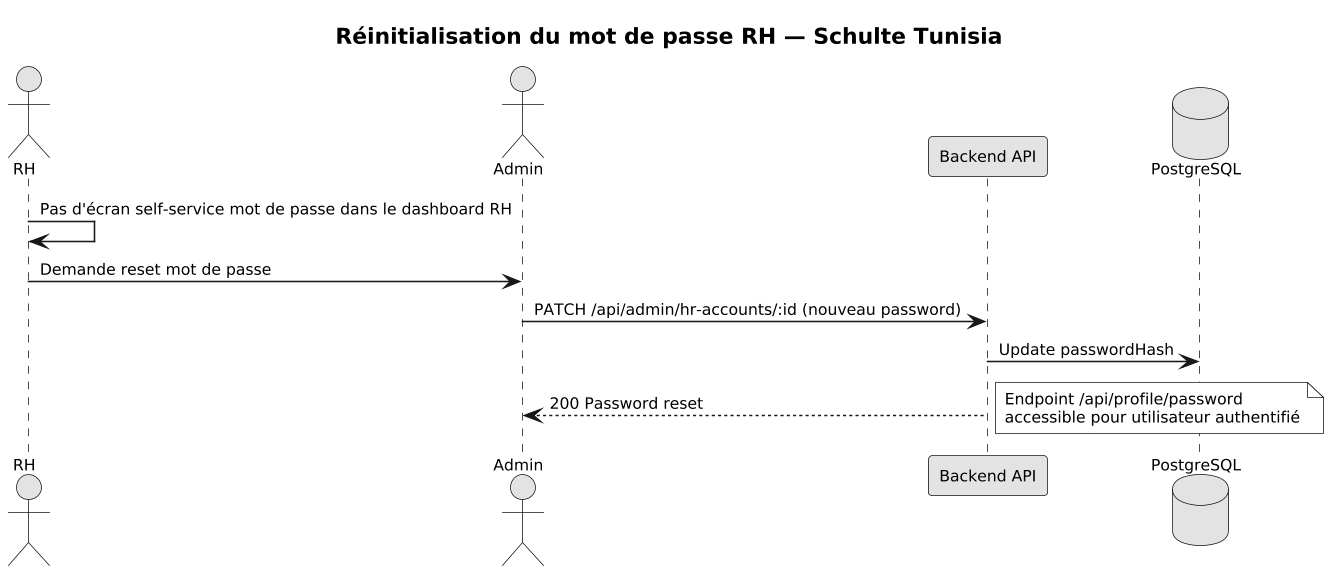
\includegraphics[width=\textwidth]{reset_mot_de_passe_rh.png}
\caption{Reset de mot de passe RH}
\end{figure}

Cette procedure permet la reprise rapide d'acces sans contournement de securite.

En complement, le front RH traite explicitement les etats de session corrompus (payload utilisateur invalide en stockage local) en nettoyant la session et en revenant a un etat non authentifie. Ce choix evite les ecrans incoherents apres fermeture navigateur ou donnees partielles.

Le controle des origines reseau suit la meme logique defensive: allowlist explicite des URLs clientes, avec options locales strictement controlees pour \texttt{localhost} et les requetes sans en-tete \texttt{Origin}. Ainsi, l'environnement de production reste ferme par defaut, tout en preservant la capacite de test en developpement.

\section{Conception des donnees}

\subsection{Modele metier}

Le modele de donnees est centre sur sept tables pivots : \texttt{Users}, \texttt{OfferTemplates}, \texttt{JobOffers}, \texttt{Applications}, \texttt{Interviews}, \texttt{Notifications}, \texttt{RefreshTokens}.

\begin{figure}[H]
\centering
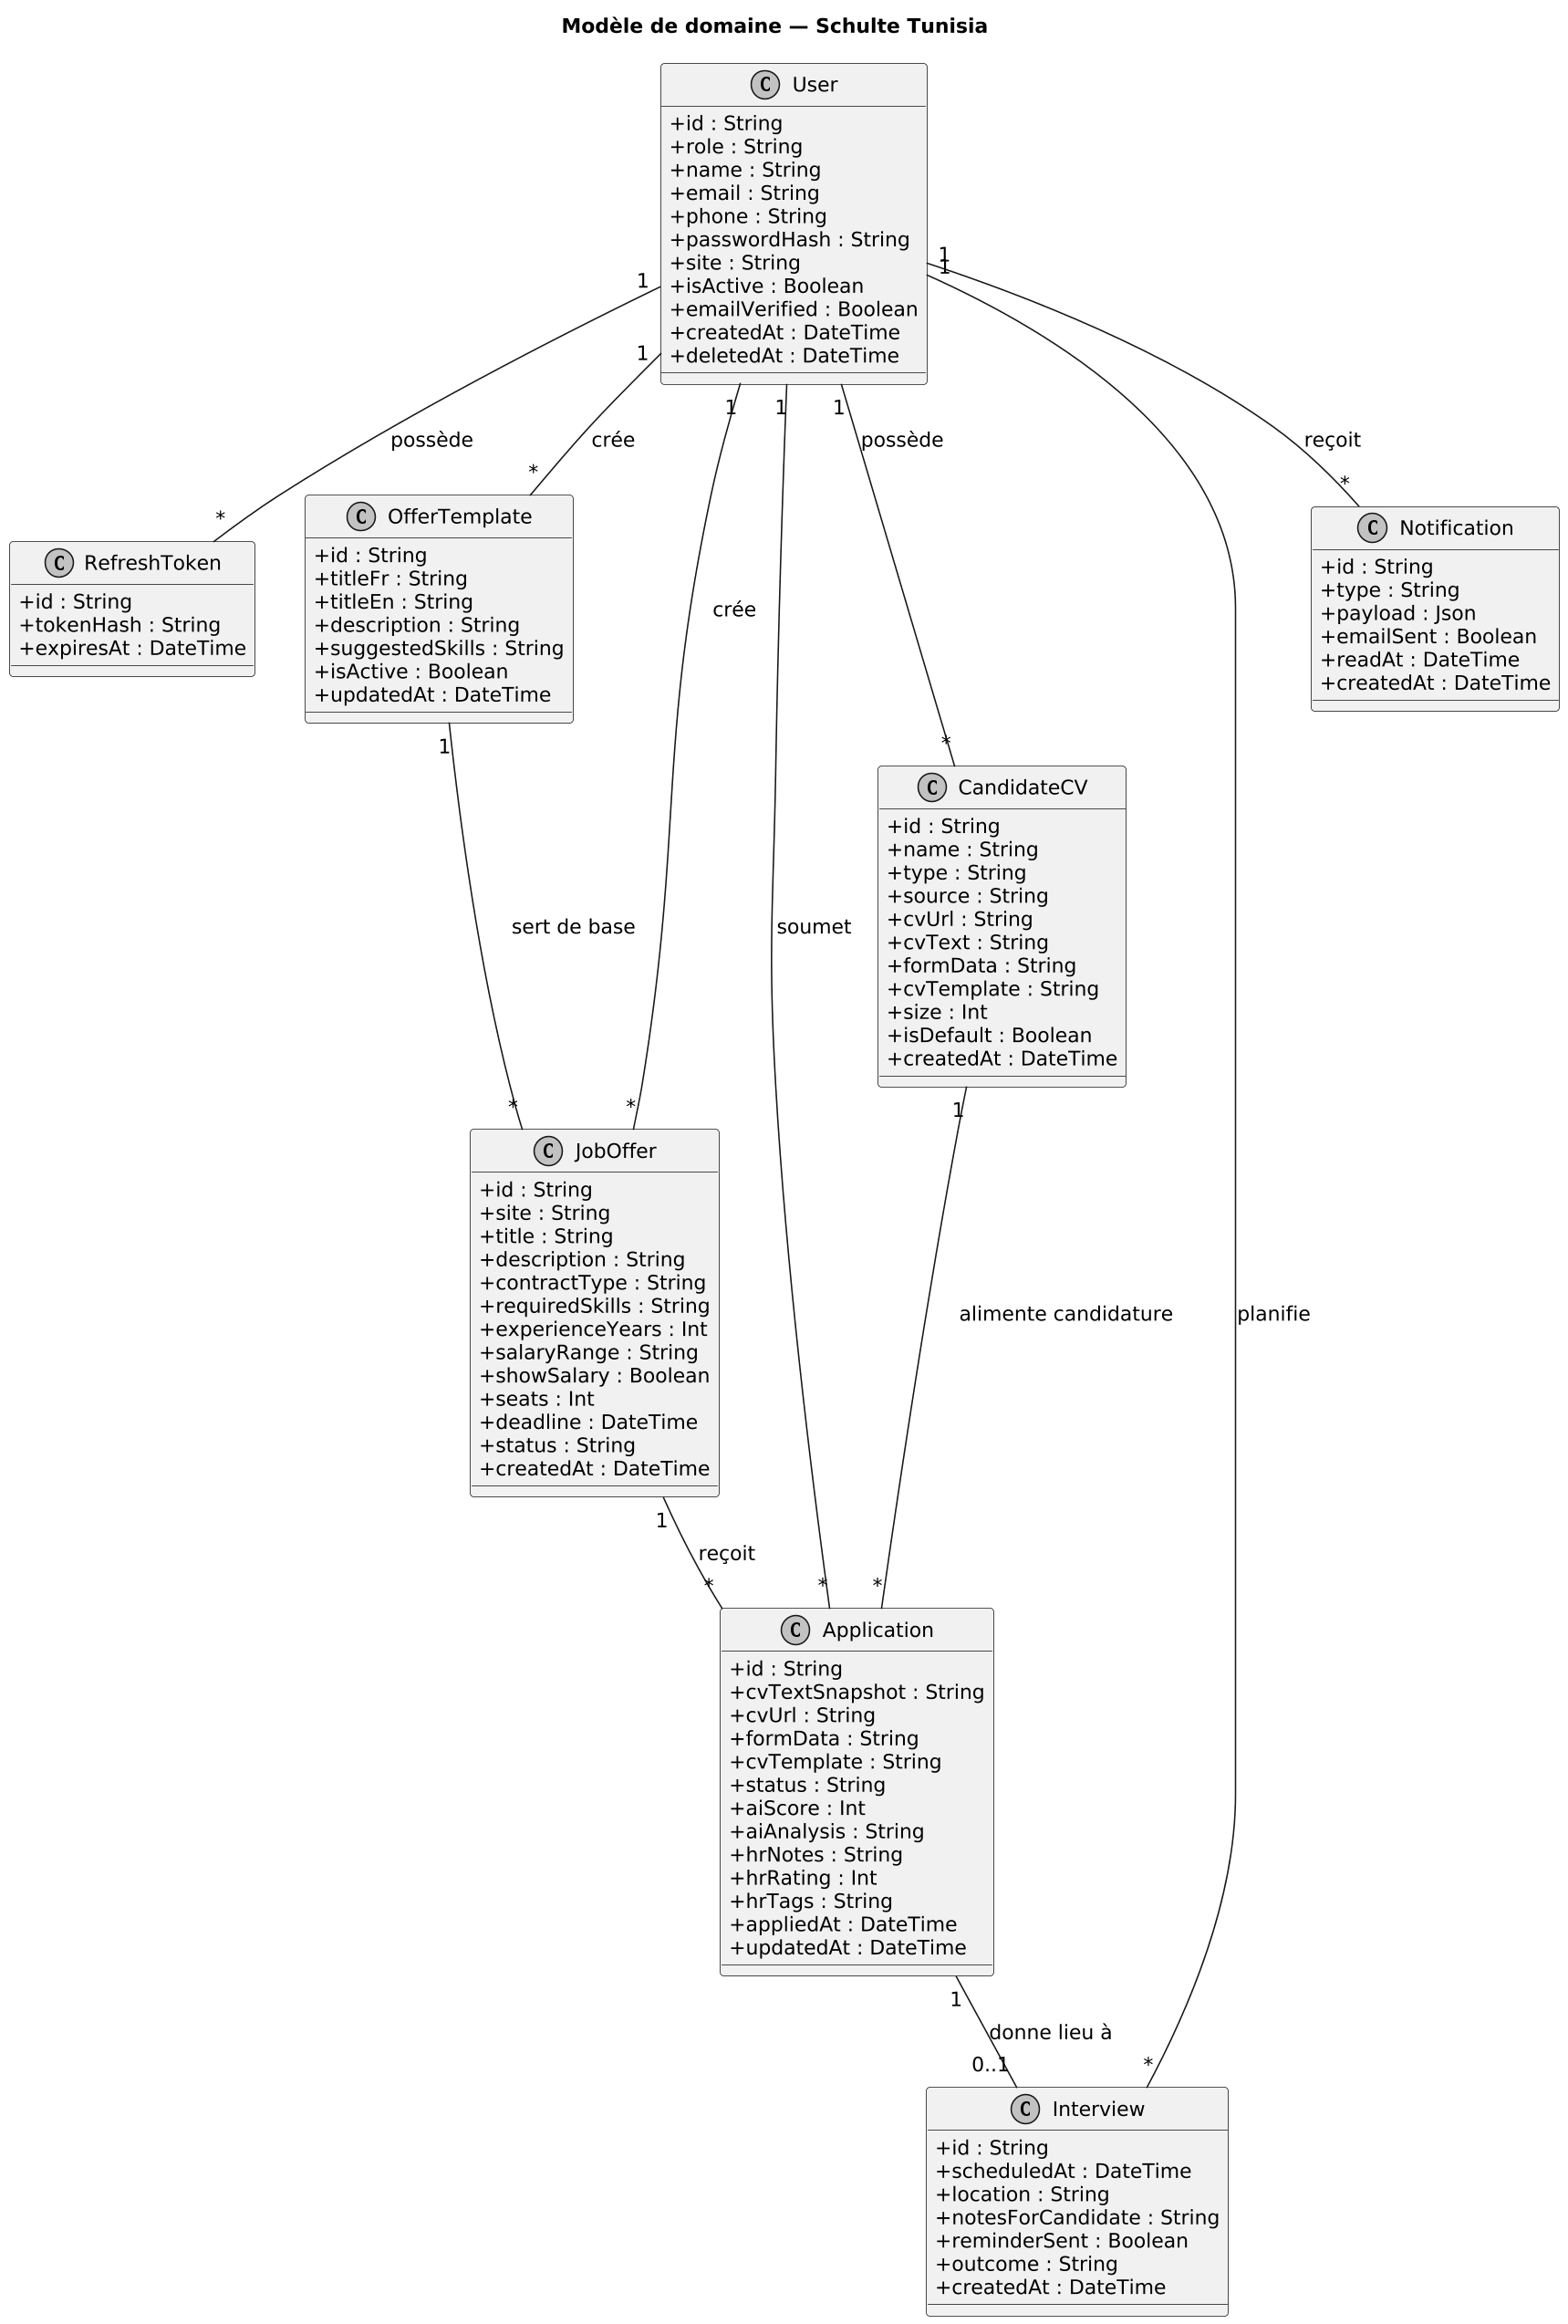
\includegraphics[width=\textwidth]{diagramme_entites_metier.png}
\caption{Diagramme des entites metier}
\end{figure}

Le diagramme mappe les objets metier et leurs relations principales.

\begin{figure}[H]
\centering
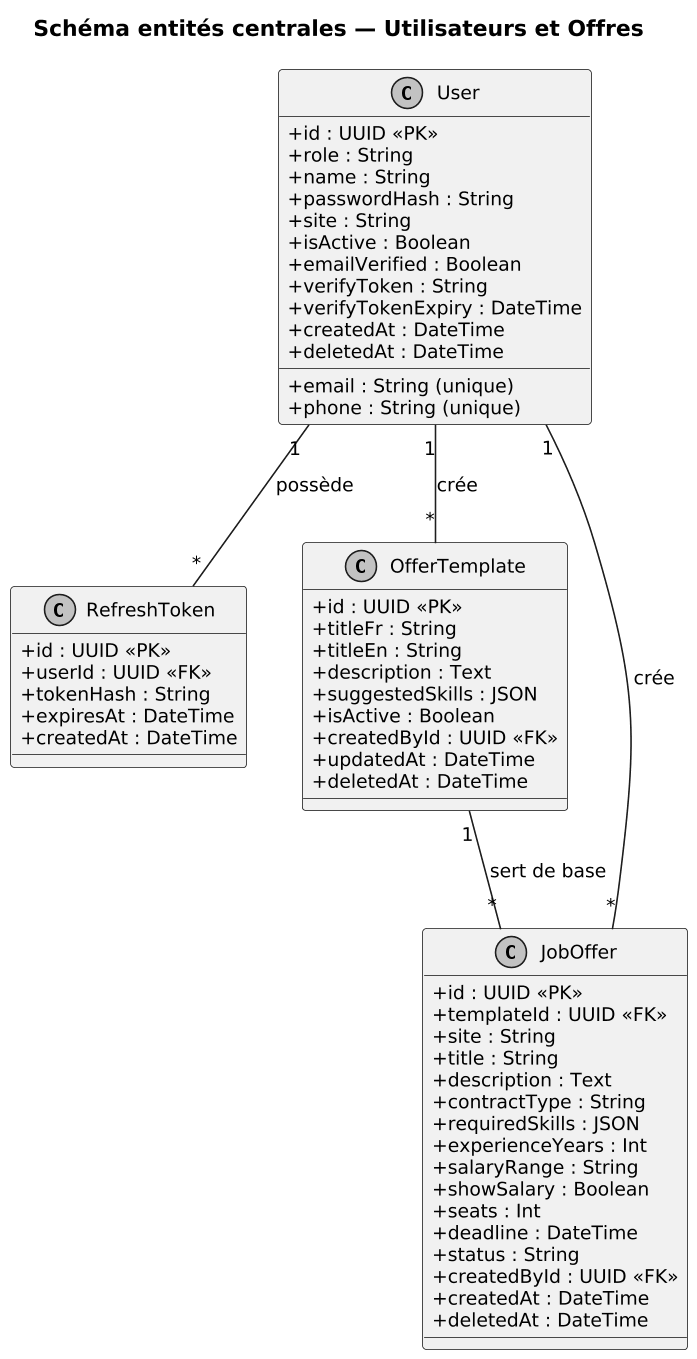
\includegraphics[width=\textwidth]{er_utilisateurs_offres.png}
\caption{Sous-modele E-R utilisateurs et offres}
\end{figure}

Nous y isolons la relation entre comptes, roles et publication d'offres.

\begin{figure}[H]
\centering
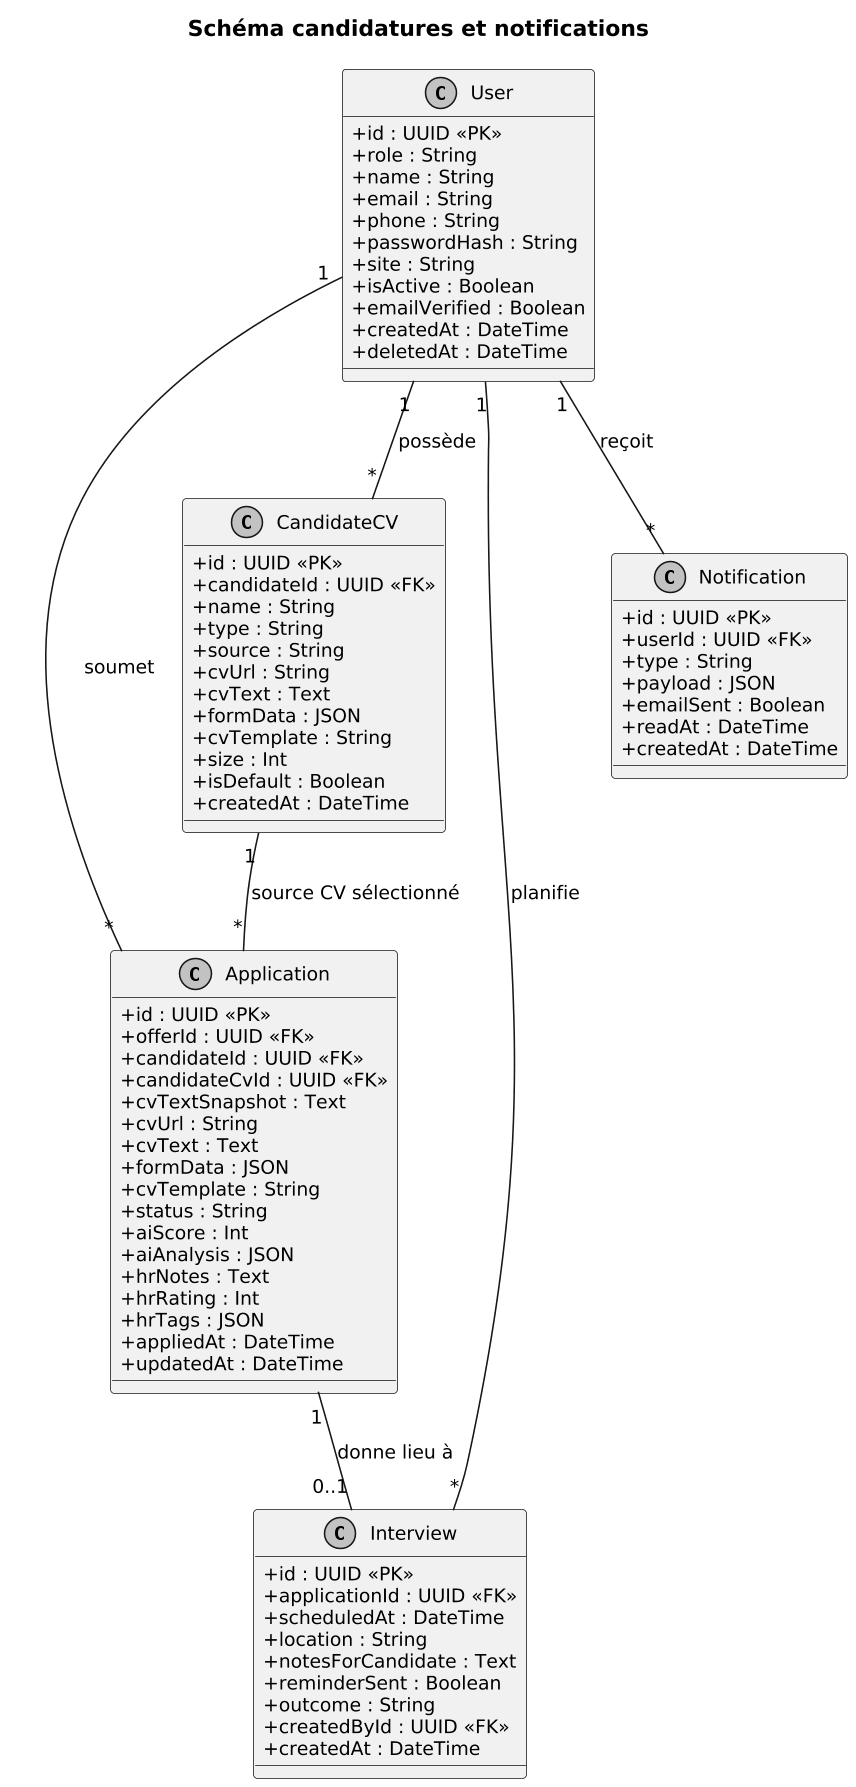
\includegraphics[width=\textwidth]{er_candidatures_cv_entretiens_notifications.png}
\caption{Sous-modele E-R candidatures, CV, entretiens et notifications}
\end{figure}

Ce sous-modele formalise le coeur du cycle de recrutement et du suivi candidat.

\subsection{Regles d'integrite}

Les regles d'integrite retenues sont explicites: unicite candidature candidat/offre, relation 1--1 candidature/entretien, rattachement d'offre a un site unique, et conservation des traces de transitions.

Un point sensible concerne le cycle de vie des CV rattaches aux candidatures. Le schema autorise la mise a \texttt{NULL} de la reference CV supprimee, mais la couche metier interdit la suppression d'un CV encore lie a une candidature active. Cette double protection (schema + regle metier) preserve a la fois l'integrite relationnelle et la coherence fonctionnelle.

La datation metier repose sur \texttt{appliedAt} pour l'ordre de traitement RH, complete par \texttt{createdAt}/\texttt{updatedAt} pour la tracabilite technique. Cote candidat, l'affichage applique un fallback robuste (\texttt{appliedAt} puis \texttt{createdAt}) avec verification de validite des dates pour eviter les rendus incoherents.

\section{Conception des composants backend}

\begin{figure}[H]
\centering
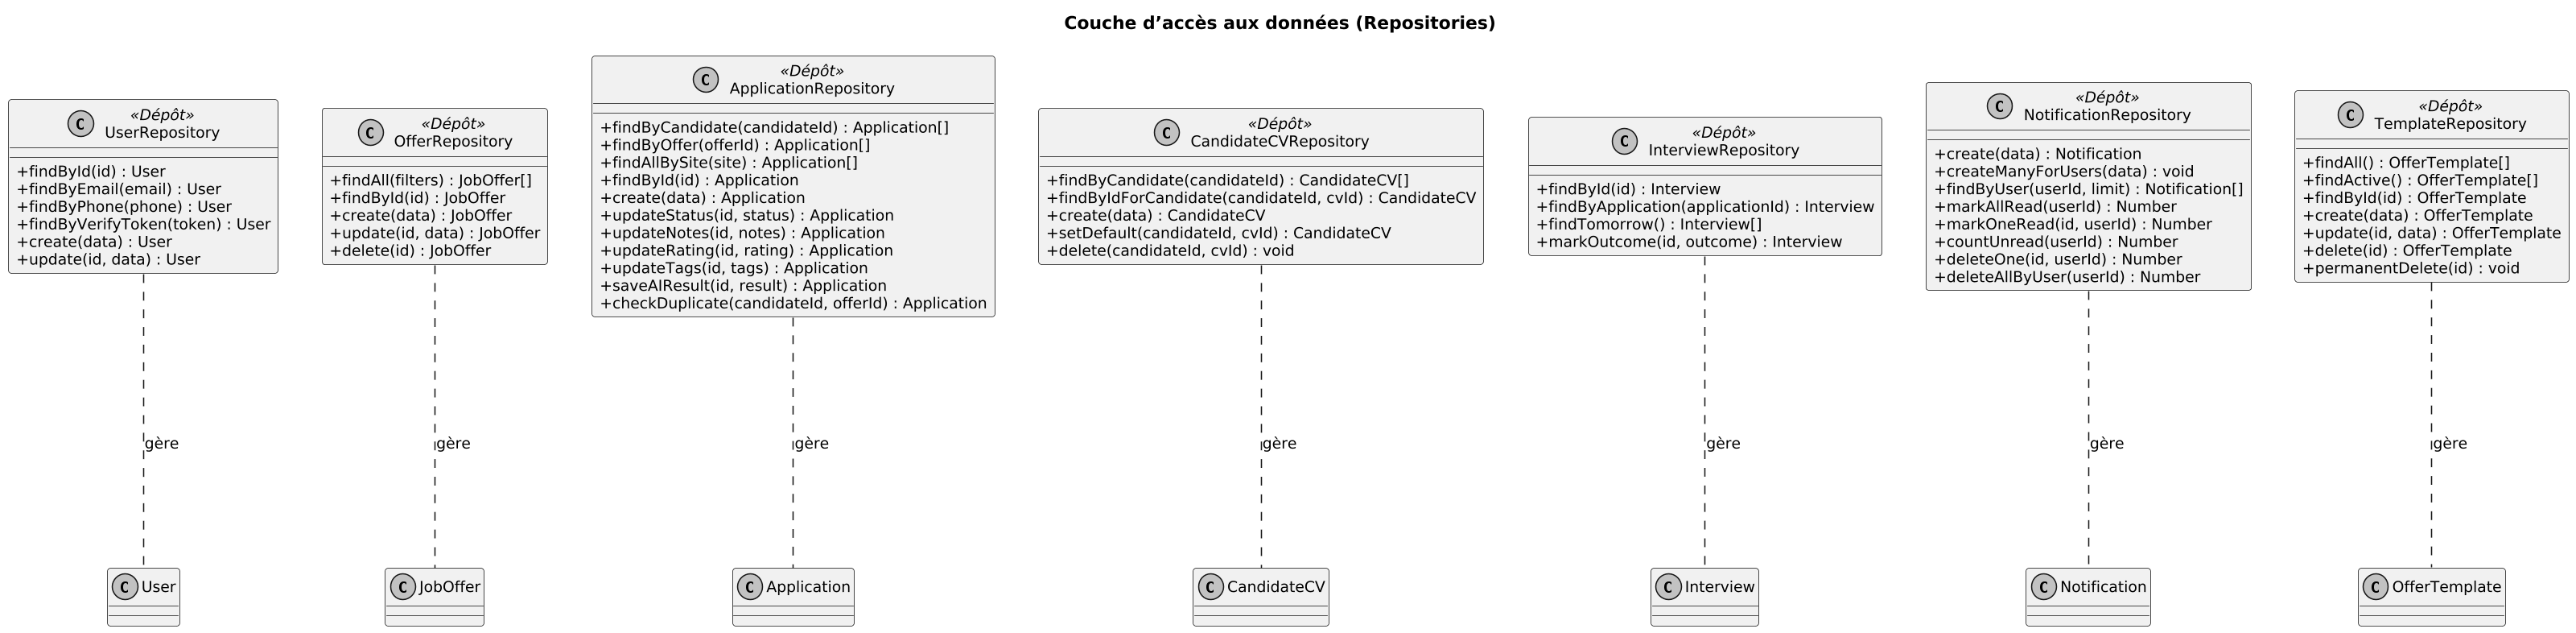
\includegraphics[width=\textwidth]{diagramme_repositories.png}
\caption{Organisation des repositories backend}
\end{figure}

Le diagramme repositories montre la separation entre acces aux donnees et logique metier.

\begin{figure}[H]
\centering
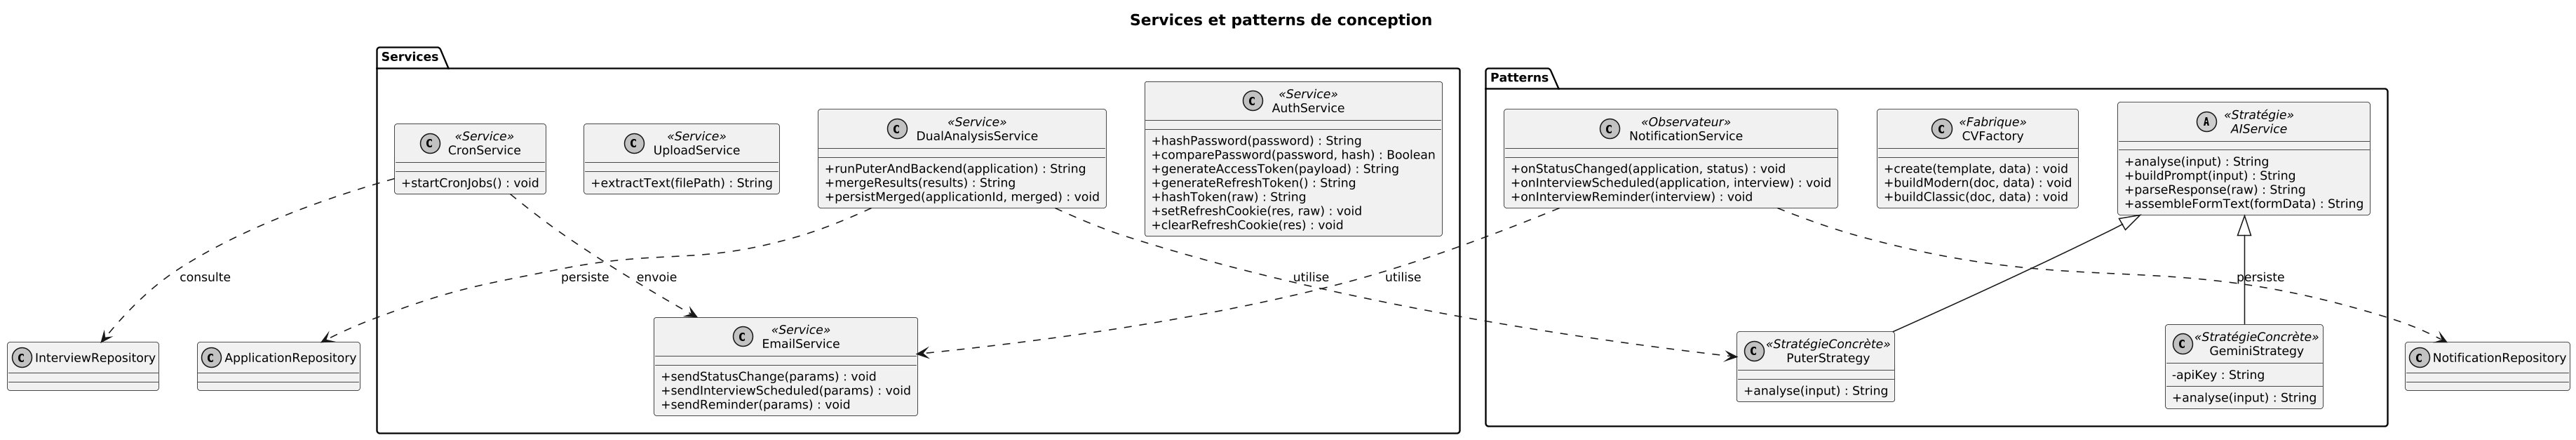
\includegraphics[width=\textwidth]{diagramme_services_patterns_conception.png}
\caption{Services applicatifs et patterns de conception}
\end{figure}

Les services sont organises par responsabilite: auth, notifications, IA, cron, upload.

La couche repository applique des selections defensives du profil candidat (\texttt{candidateSafeSelect}) pour exclure les attributs sensibles des objets retournes aux ecrans RH/Admin. Cette pratique complete l'autorisation: meme en cas d'acces valide, seules les donnees necessaires au cas d'usage sont exposees.

Pour les operations de masse, la conception impose des garde-fous explicites: validation des identifiants, dedoublonnage, plafond de taille de lot, verification de perimetre site pour les RH, puis execution transactionnelle. Cette sequence evite les mises a jour partielles et limite les effets de bord sur les campagnes de tri en volume.

\begin{figure}[H]
\centering
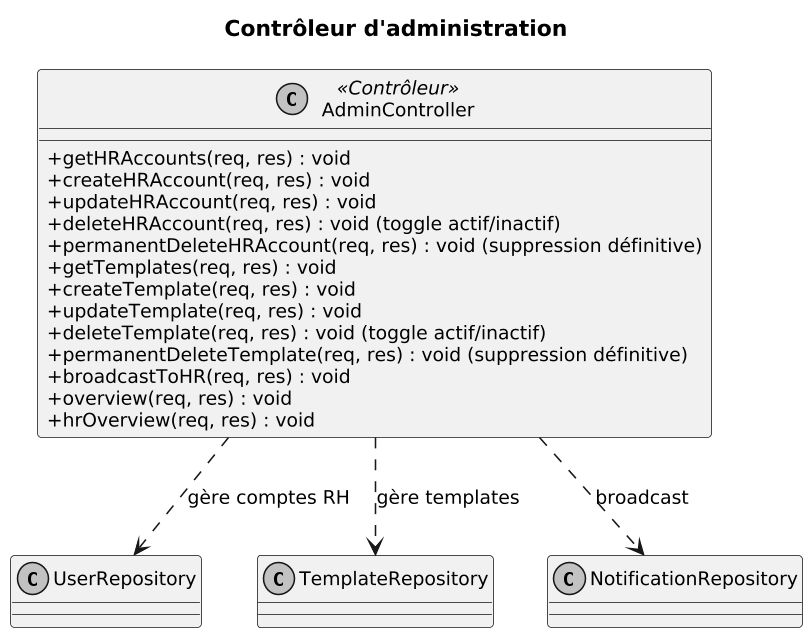
\includegraphics[width=\textwidth]{diagramme_controleur_admincontroller.png}
\caption{Conception detaillee du controleur d'administration}
\end{figure}

La vue du controleur admin illustre l'orchestration des operations de gouvernance : comptes RH, templates, suppression logique ou definitive, et broadcast.

La conception backend applique aussi une sanitisation explicite des objets candidats selon le contexte de consultation (liste, entretien, detail), afin d'eviter toute fuite de champs sensibles dans les reponses API.

Sur les endpoints lourds (offres, entretiens), la pagination (\texttt{limit} + \texttt{cursor}) est integree des la conception backend. L'objectif est double: contenir le cout des requetes volumineuses et permettre un chargement incrementiel stable cote frontend, sans rupture de compatibilite quand les parametres sont absents.

\section{Conception RH/Admin et gouvernance}

\begin{figure}[H]
\centering
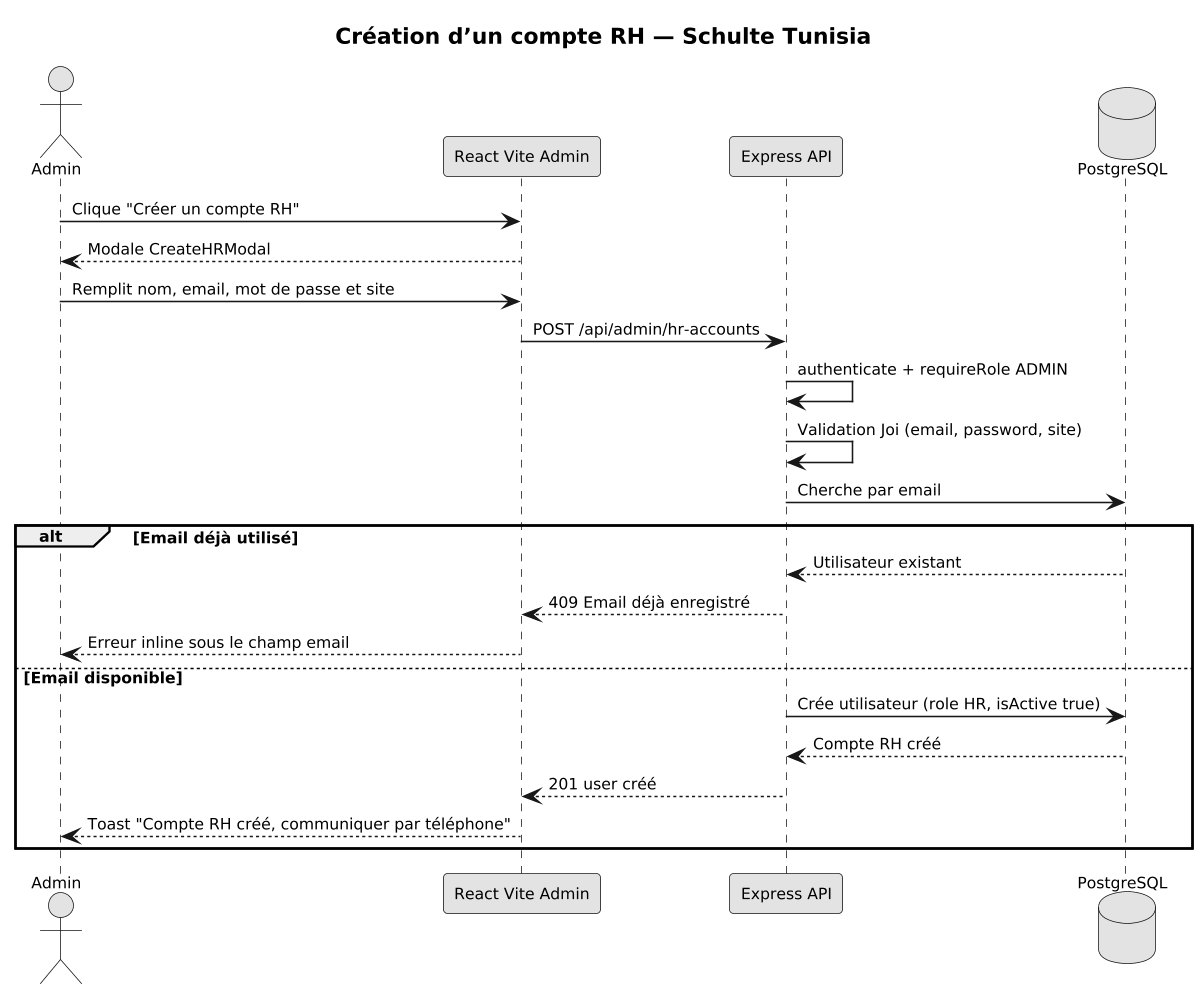
\includegraphics[width=\textwidth]{creation_compte_rh.png}
\caption{Creation d'un compte RH}
\end{figure}

La creation de compte RH est reservee a l'administration avec contraintes de role et controle d'unicite email.

Le perimetre RH est ensuite contraint par site: un RH ne peut agir que sur les offres et candidatures de son site. Cote creation d'offre, l'utilisation d'un template actif est imposee pour les comptes RH, ce qui garantit un cadre de publication homogene et controle par l'administration.

\begin{figure}[H]
\centering
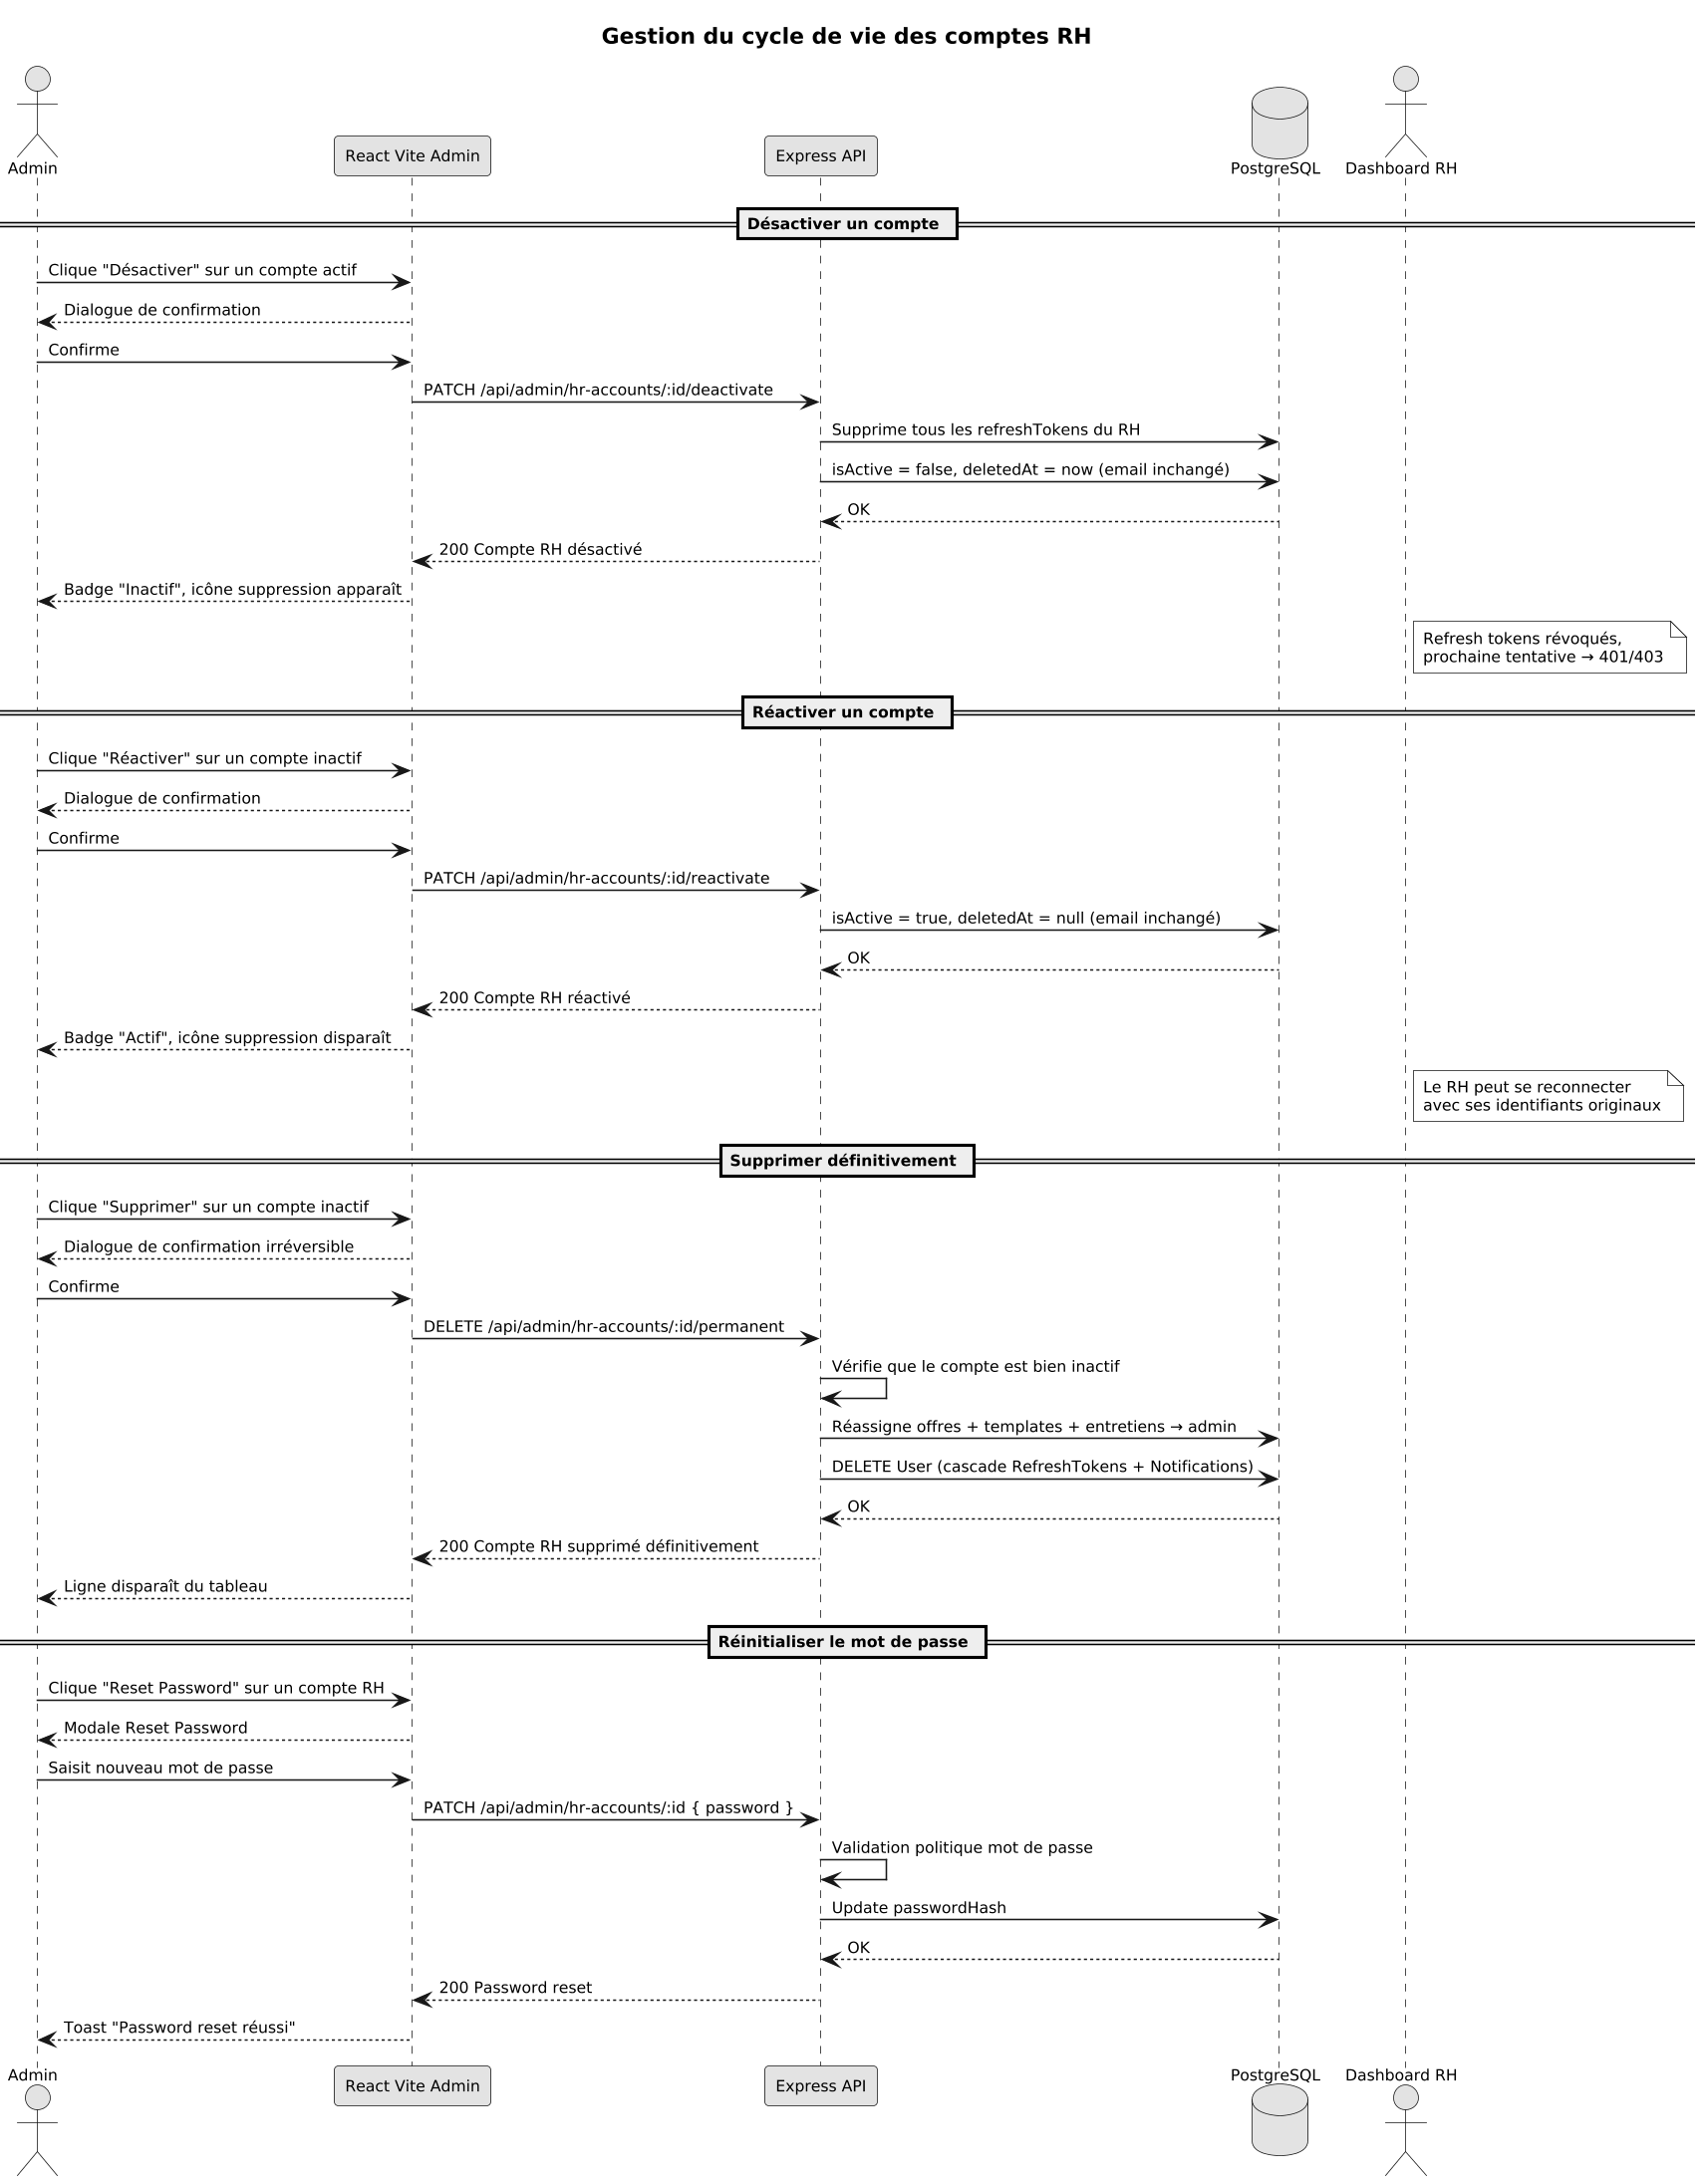
\includegraphics[width=\textwidth]{cycle_vie_compte_rh.png}
\caption{Cycle de vie d'un compte RH}
\end{figure}

Le cycle RH formalise activation, desactivation et reactivation pour eviter les etats implicites.

\begin{figure}[H]
\centering
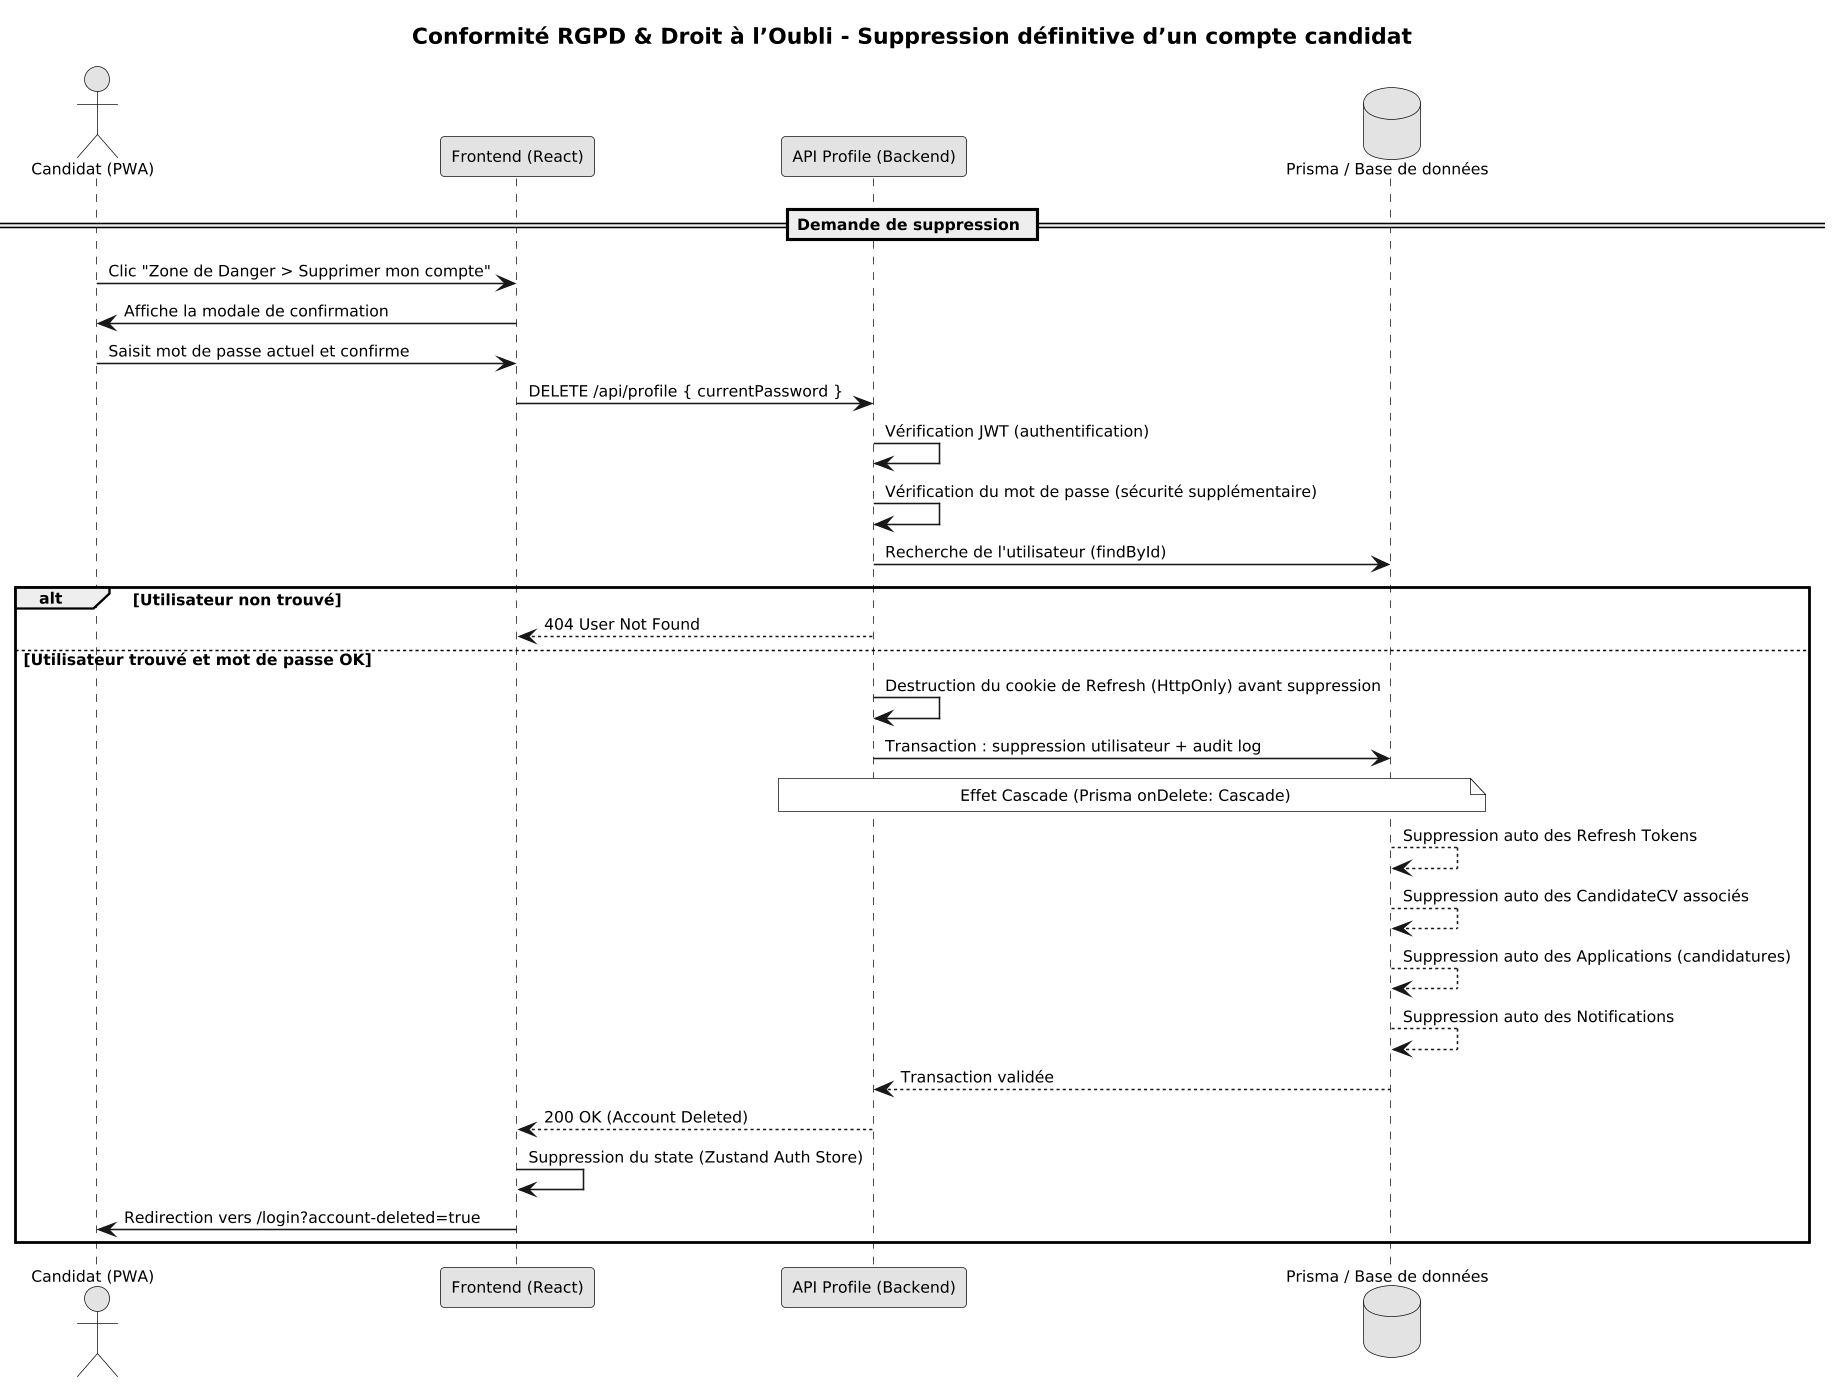
\includegraphics[width=\textwidth]{flux_suppression_compte.png}
\caption{Flux de suppression de compte RH}
\end{figure}

La suppression suit un flux controle pour conserver la coherence des donnees dependantes.

\begin{figure}[H]
\centering
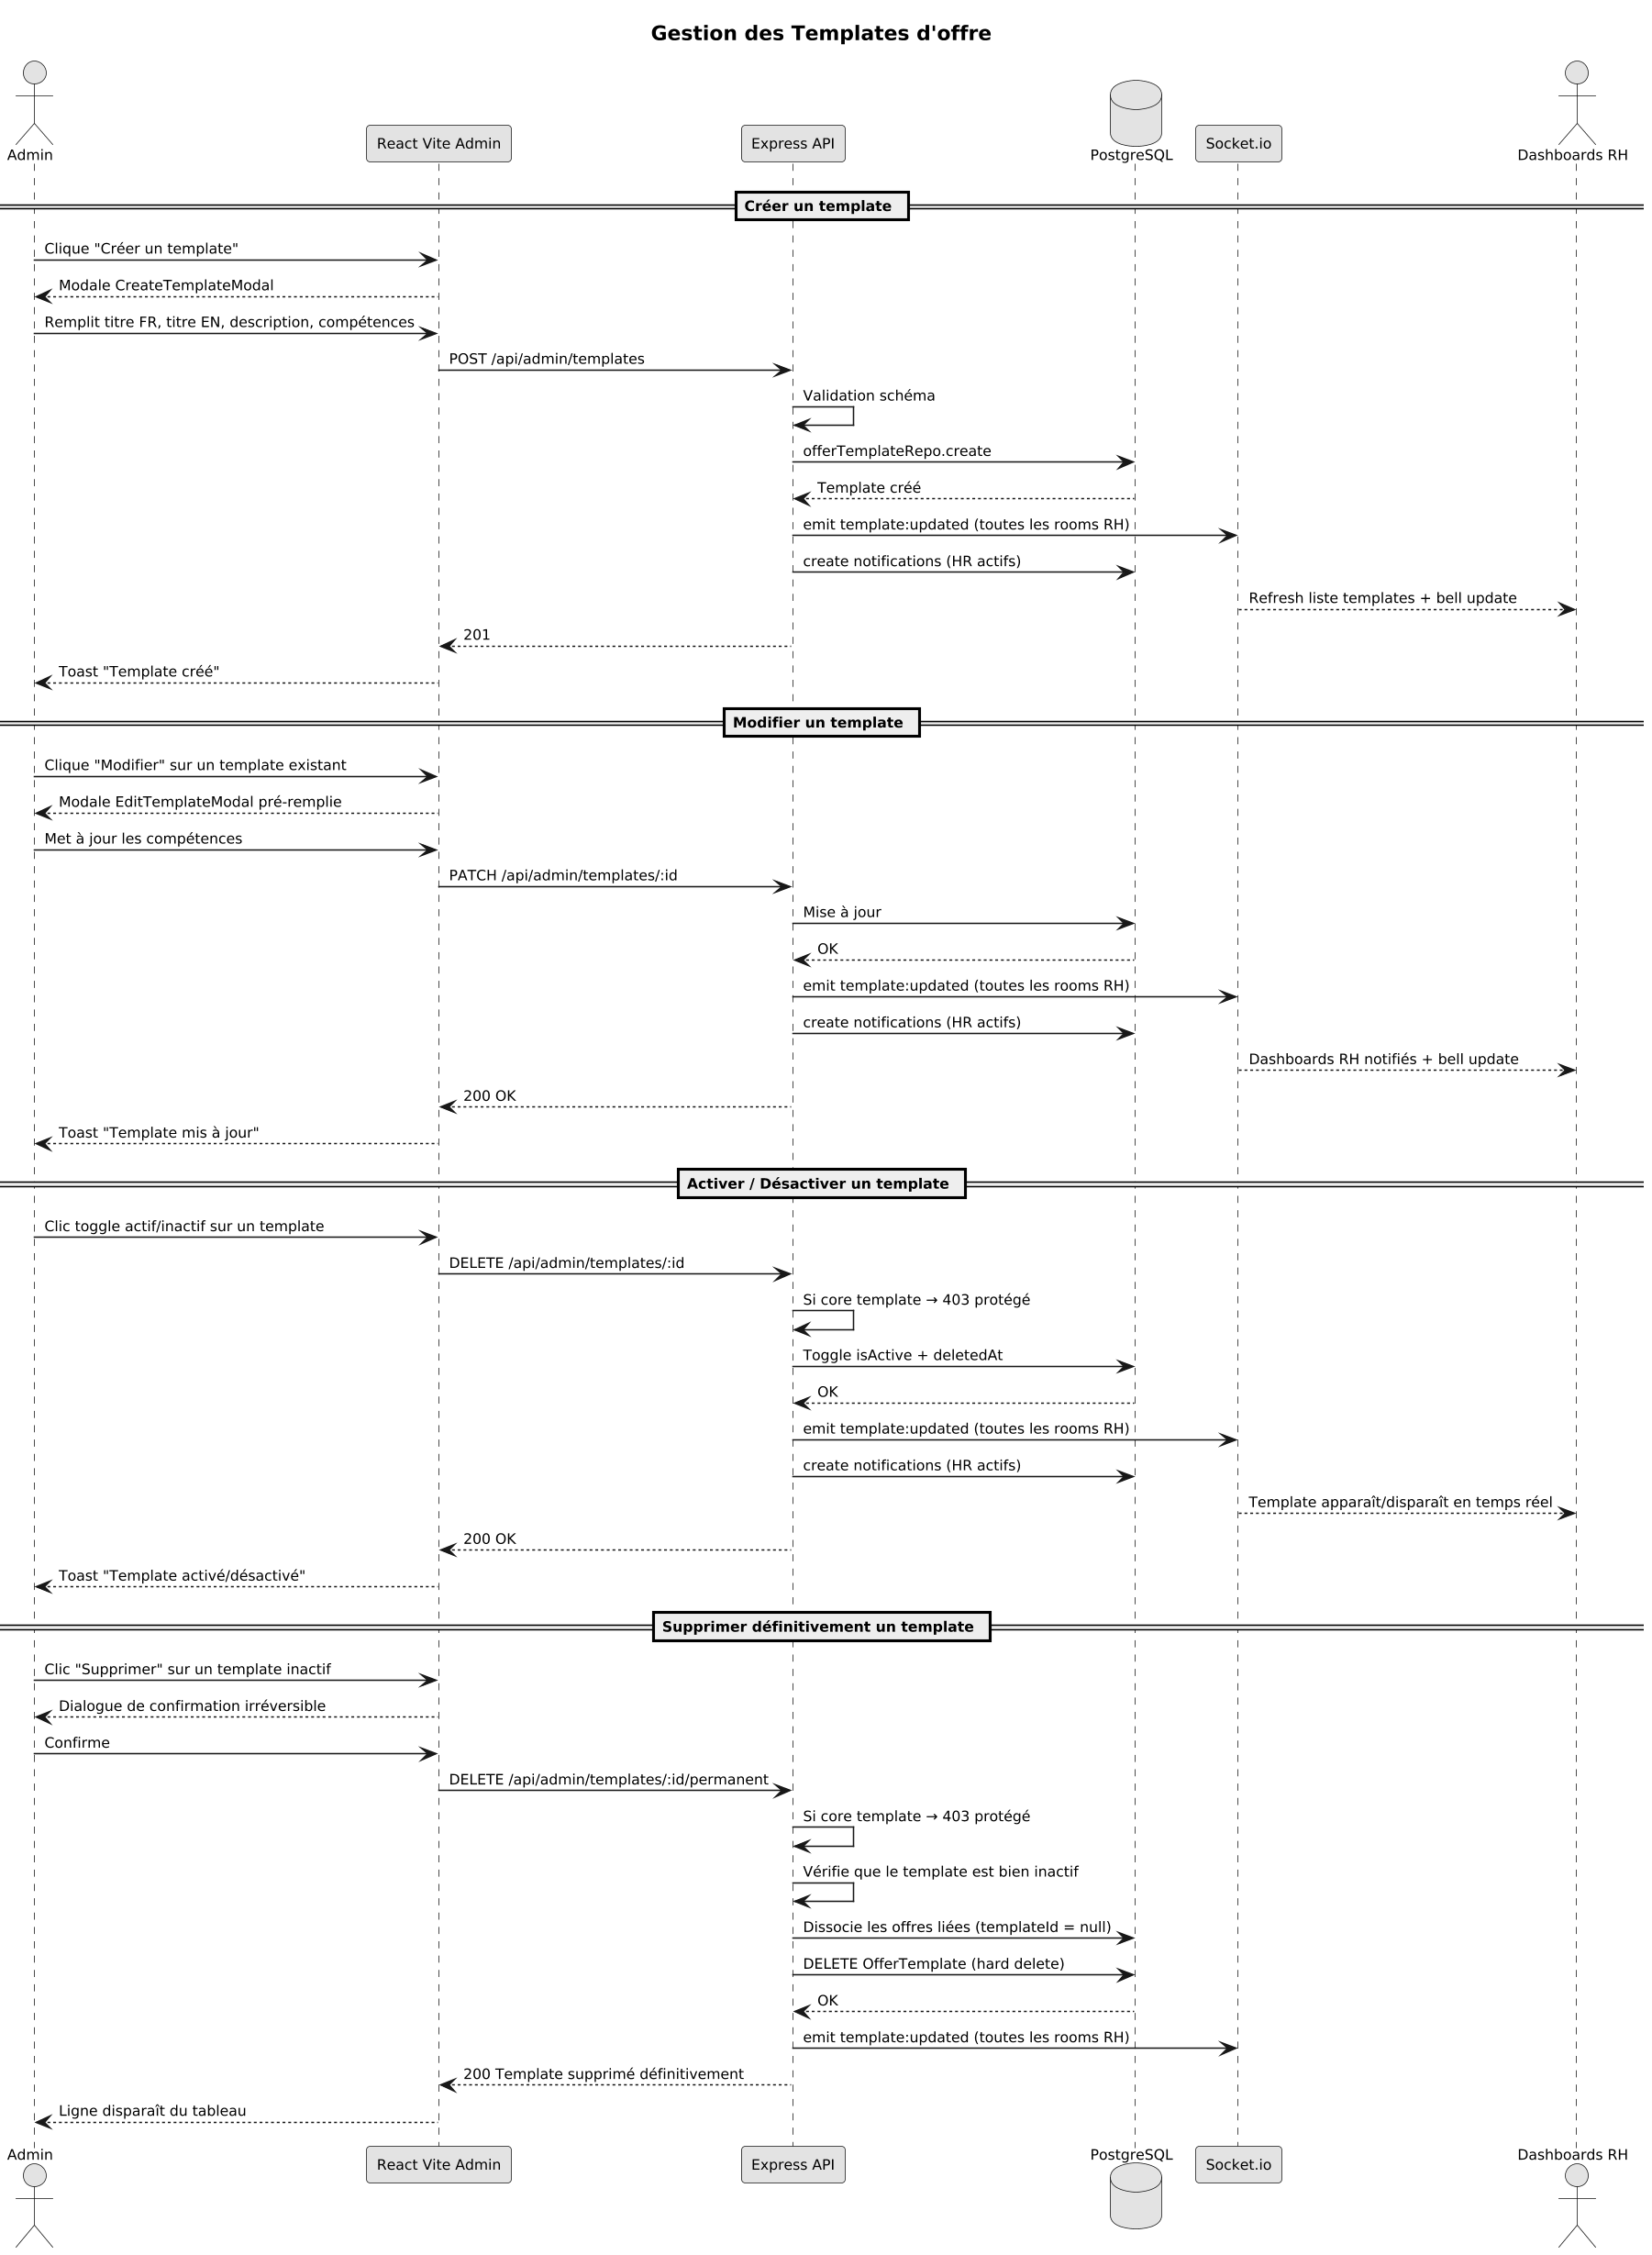
\includegraphics[width=\textwidth]{gestion_templates.png}
\caption{Gestion des templates d'offres}
\end{figure}

Les templates accelerent la publication tout en gardant un cadre commun entre sites.

\begin{figure}[H]
\centering
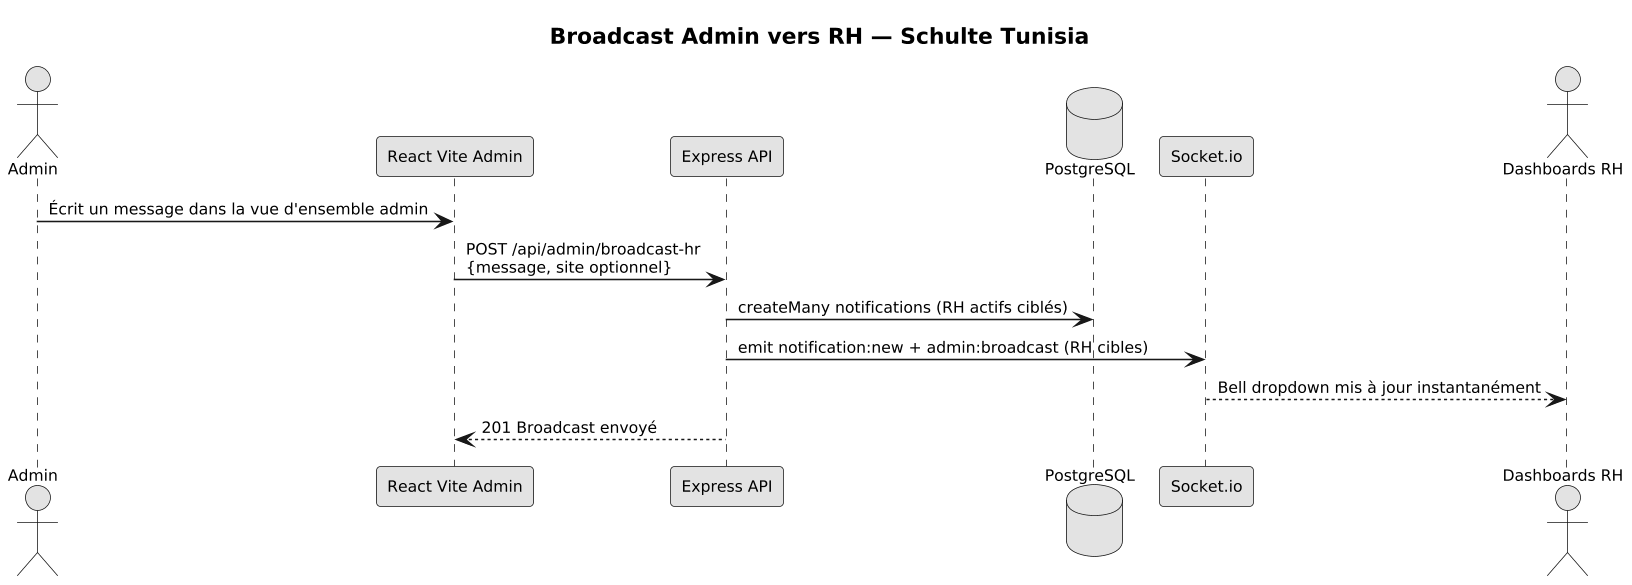
\includegraphics[width=\textwidth]{broadcast_admin_vers_rh.png}
\caption{Broadcast admin vers RH}
\end{figure}

Ce flux couvre la diffusion d'informations transversales vers les equipes RH.

\section{Notifications et automatisation}

\begin{figure}[H]
\centering
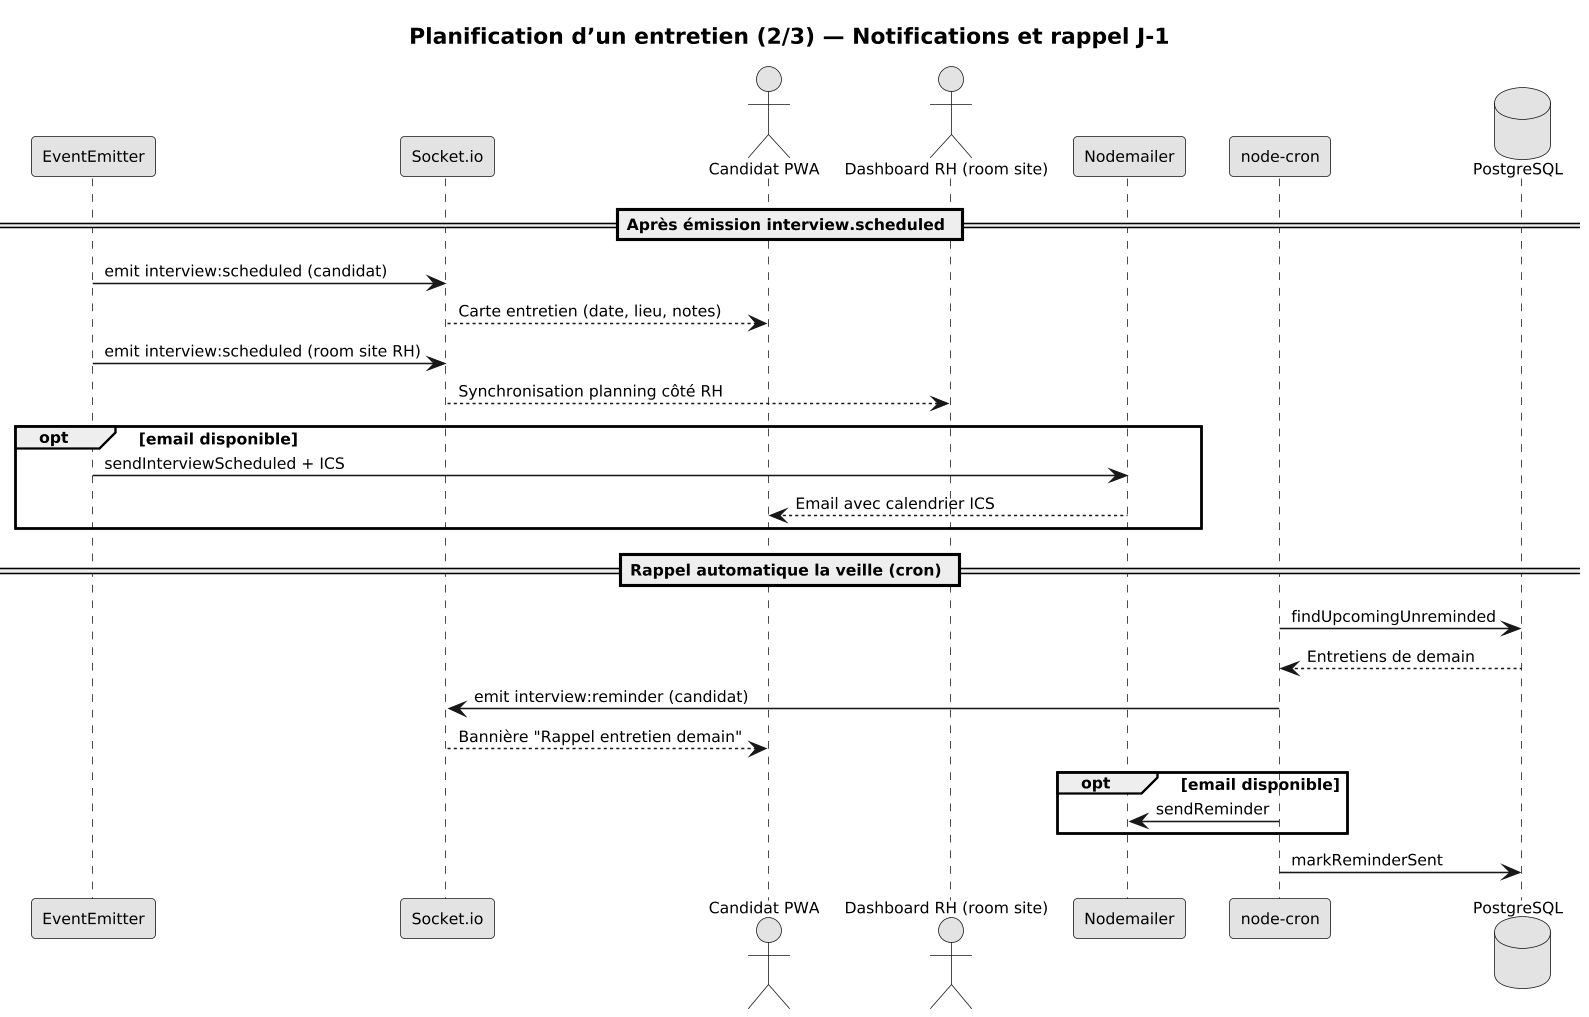
\includegraphics[width=\textwidth]{notifications_rappel_automatique.png}
\caption{Conception des notifications et rappels}
\end{figure}

Nous combinons notifications metier immediates et rappels planifies pour eviter les oublis operatoires.

La chaine de notification est bi-canal: persistance en base (historique, non-lus) puis emission Socket ciblee vers l'acteur concerne. Si le client est temporairement hors ligne, l'etat reste recuperable via l'API \texttt{/notifications}, dont la reponse est bornee par un \texttt{limit} pour maitriser la charge.

\begin{figure}[H]
\centering
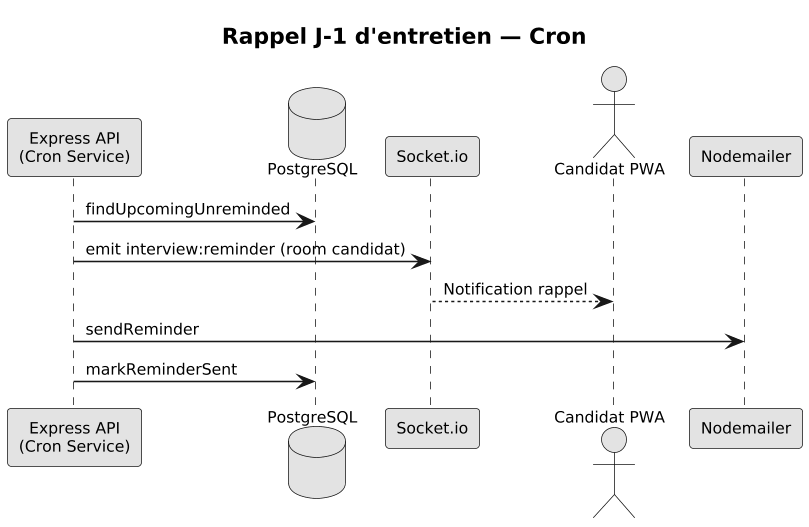
\includegraphics[width=\textwidth]{rappel_automatique_entretien.png}
\caption{Rappel automatique d'entretien}
\end{figure}

Le rappel d'entretien est planifie automatiquement (cron) pour fiabiliser la presence aux rendez-vous.

Du cote client candidat, les actions de lecture/suppression de notifications utilisent un mecanisme d'optimistic update avec rollback en cas d'echec API. Cette decision de conception maintient une interface reactive sans sacrifier la coherence finale des donnees affichees.

\section{Synthese des choix de conception}

\begin{table}[H]
\centering
\caption{Traçabilite exigences -> conception}
\begin{tabularx}{\textwidth}{|l|X|X|}
\hline
\textbf{Exigence} & \textbf{Traduction conception} & \textbf{Preuve UML / composant} \\
\hline
Depot candidature fluide & Soumission asynchrone + analyse IA en arriere-plan & Diagrammes de depot, analyse asynchrone et normalisation \\
\hline
Isolement multi-site RH & Verification role/site sur routes sensibles & Diagrammes RH, entretiens et couche d'autorisation \\
\hline
Suivi temps reel & Diffusion Socket.io ciblee & Architecture temps reel + diagrammes de transitions \\
\hline
Cycle entretien traçable & Etats explicites + transitions controlees & Diagrammes d'etats et d'entretien \\
\hline
Securite d'acces & JWT court + refresh rotation + revocation & Diagrammes d'authentification et de revocation \\
\hline
\end{tabularx}
\end{table}

\subsection{Verification croisee conception-code}

Pour limiter l'ecart entre la conception et l'implementation reelle, nous avons aligne les decisions d'architecture sur des points de controle observables dans le code. Cette verification croisee rend les choix defendables, car chaque principe peut etre rattache a un mecanisme concret.

\begin{table}[H]
\centering
\caption{Matrice de verification conception -> implementation}
\begin{tabularx}{\textwidth}{|l|X|X|}
\hline
\textbf{Axe} & \textbf{Choix de conception} & \textbf{Mecanisme implemente} \\
\hline
Session securisee & Acces court + refresh avec rotation & Suppression de l'ancien refresh token, emission d'un nouveau, cookie \texttt{HttpOnly} borne a \texttt{/api/auth/refresh}. \\
\hline
Isolement multi-site & RH limite a son perimetre & Verifications role/site sur lectures et actions sensibles; rejet explicite des acces inter-site. \\
\hline
Coherence des statuts & Transitions maitrisees & Normalisation \texttt{review -> reviewing}, blocage des cas terminaux pour la planification, et controles en lot transactionnels. \\
\hline
Temps reel fiable & Notification ciblee par acteur & Rooms Socket par role/site/utilisateur, plus persistance DB pour reprise apres deconnexion client. \\
\hline
Scalabilite lecture & Limiter les charges volumineuses & Parametres \texttt{limit}/\texttt{cursor} sur endpoints lourds (offres, entretiens, notifications). \\
\hline
\end{tabularx}
\end{table}

\subsection{Hypotheses et limites de conception}

La conception retenue est adaptee au contexte actuel du projet et de l'entreprise. Elle repose sur des hypotheses explicites, qui delimitent aussi ses limites:
\begin{itemize}
  \item le perimetre metier cible deux sites (Bouarada et Zaghouan) avec des roles RH/Admin/Candidat bien separes;
  \item la plateforme privilegie la cohesion fonctionnelle d'un backend central, sans decomposition microservices;
  \item l'analyse IA reste un outil d'aide a la decision, et non un mecanisme de decision automatique;
  \item la strategie temps reel est basee sur Socket.io, sans ajout d'un bus de messages externe dans cette phase;
  \item la robustesse en echec est traitee au niveau applicatif (fallbacks, rollback UI, validations), sans infrastructure distribuee additionnelle.
\end{itemize}

Ces limites sont assumees dans la phase PFE pour conserver un niveau de complexite compatible avec les objectifs academiques et les contraintes de delai, tout en garantissant une base evolutive pour les perspectives du chapitre suivant.

\section{Conclusion}

Ce chapitre a etabli une conception complete de la solution, depuis la planification jusqu'aux choix d'architecture et de securite. Les modeles UML, les tableaux Agile et les regles d'integrite presentes ici ont servi de cadre de reference pour la realisation.

L'apport principal de cette conception tient a la formalisation des cas limites: isolation inter-site, protection des etats terminaux, validation stricte des CV, gestion transactionnelle des actions en lot, et comportement robuste en cas d'erreur de session ou de notification. Le chapitre suivant presente la mise en oeuvre de ces choix et les validations obtenues en execution.
